\documentclass[12pt,UTF8]{ctexart}
\usepackage{ctex,amsmath,amssymb,geometry,fancyhdr,bm,amsfonts
,mathtools,extarrows,graphicx,url,enumerate,color,float,multicol,,subfig} 
\allowdisplaybreaks[4]
% 加入中文支持
\newcommand\Set[2]{%
\left\{#1\ \middle\vert\ #2 \right\}}
\geometry{a4paper,scale=0.80}
\pagestyle{fancy}
\rhead{习题7.5\&7.6\&7.7}
\lhead{基础习题课讲义}
\chead{微积分B(1)}
\begin{document}
\setcounter{section}{10}
\section{定积分(2)}
\noindent
\subsection{知识结构}
\noindent第7章定积分
	\begin{enumerate}
		\item[7.5]定积分的几何应用
			\begin{enumerate}
				\item[7.5.1]平面图形的面积
				\item[7.5.2]曲线长度的计算
				\item[7.5.3]平面曲线的曲率
				\item[7.5.4]旋转体的体积与旋转曲面的面积
			\end{enumerate}
		\item[7.6]定积分的物理应用
		\item[7.7]反常积分
			\begin{enumerate}
				\item[7.7.1]无穷积分
				\item[7.7.2]瑕积分
				\item[7.7.3]反常积分的收敛性的判定
			\end{enumerate}
	\end{enumerate}
\subsection{习题7.5解答}
\begin{enumerate}
\item求下列曲线所围图形的面积:
\newline
(1)$y=x^2$与$y=2-x^2$;
\newline
(2)$y=|\ln x|,y=0,x=\frac1{10}$及$x=10$;
\newline
(3)蚌线$\rho=a\cos\theta+b,b\geq a>0$;
\newline
(4)$\frac{x^2}{a^2}+\frac{y^2}{b^2}=1,a>0,b>0$;
\newline
(5)$\sqrt{\frac xa}+\sqrt{\frac yb}=1,a,b>0,x=0,y=0$.

解:(1)由$x^2=2-x^2$得两曲线的交点为$(\pm1,1)$,两曲线围成的图形如图~\ref{5-1-1}所示,
\begin{figure}[H]
\begin{center}
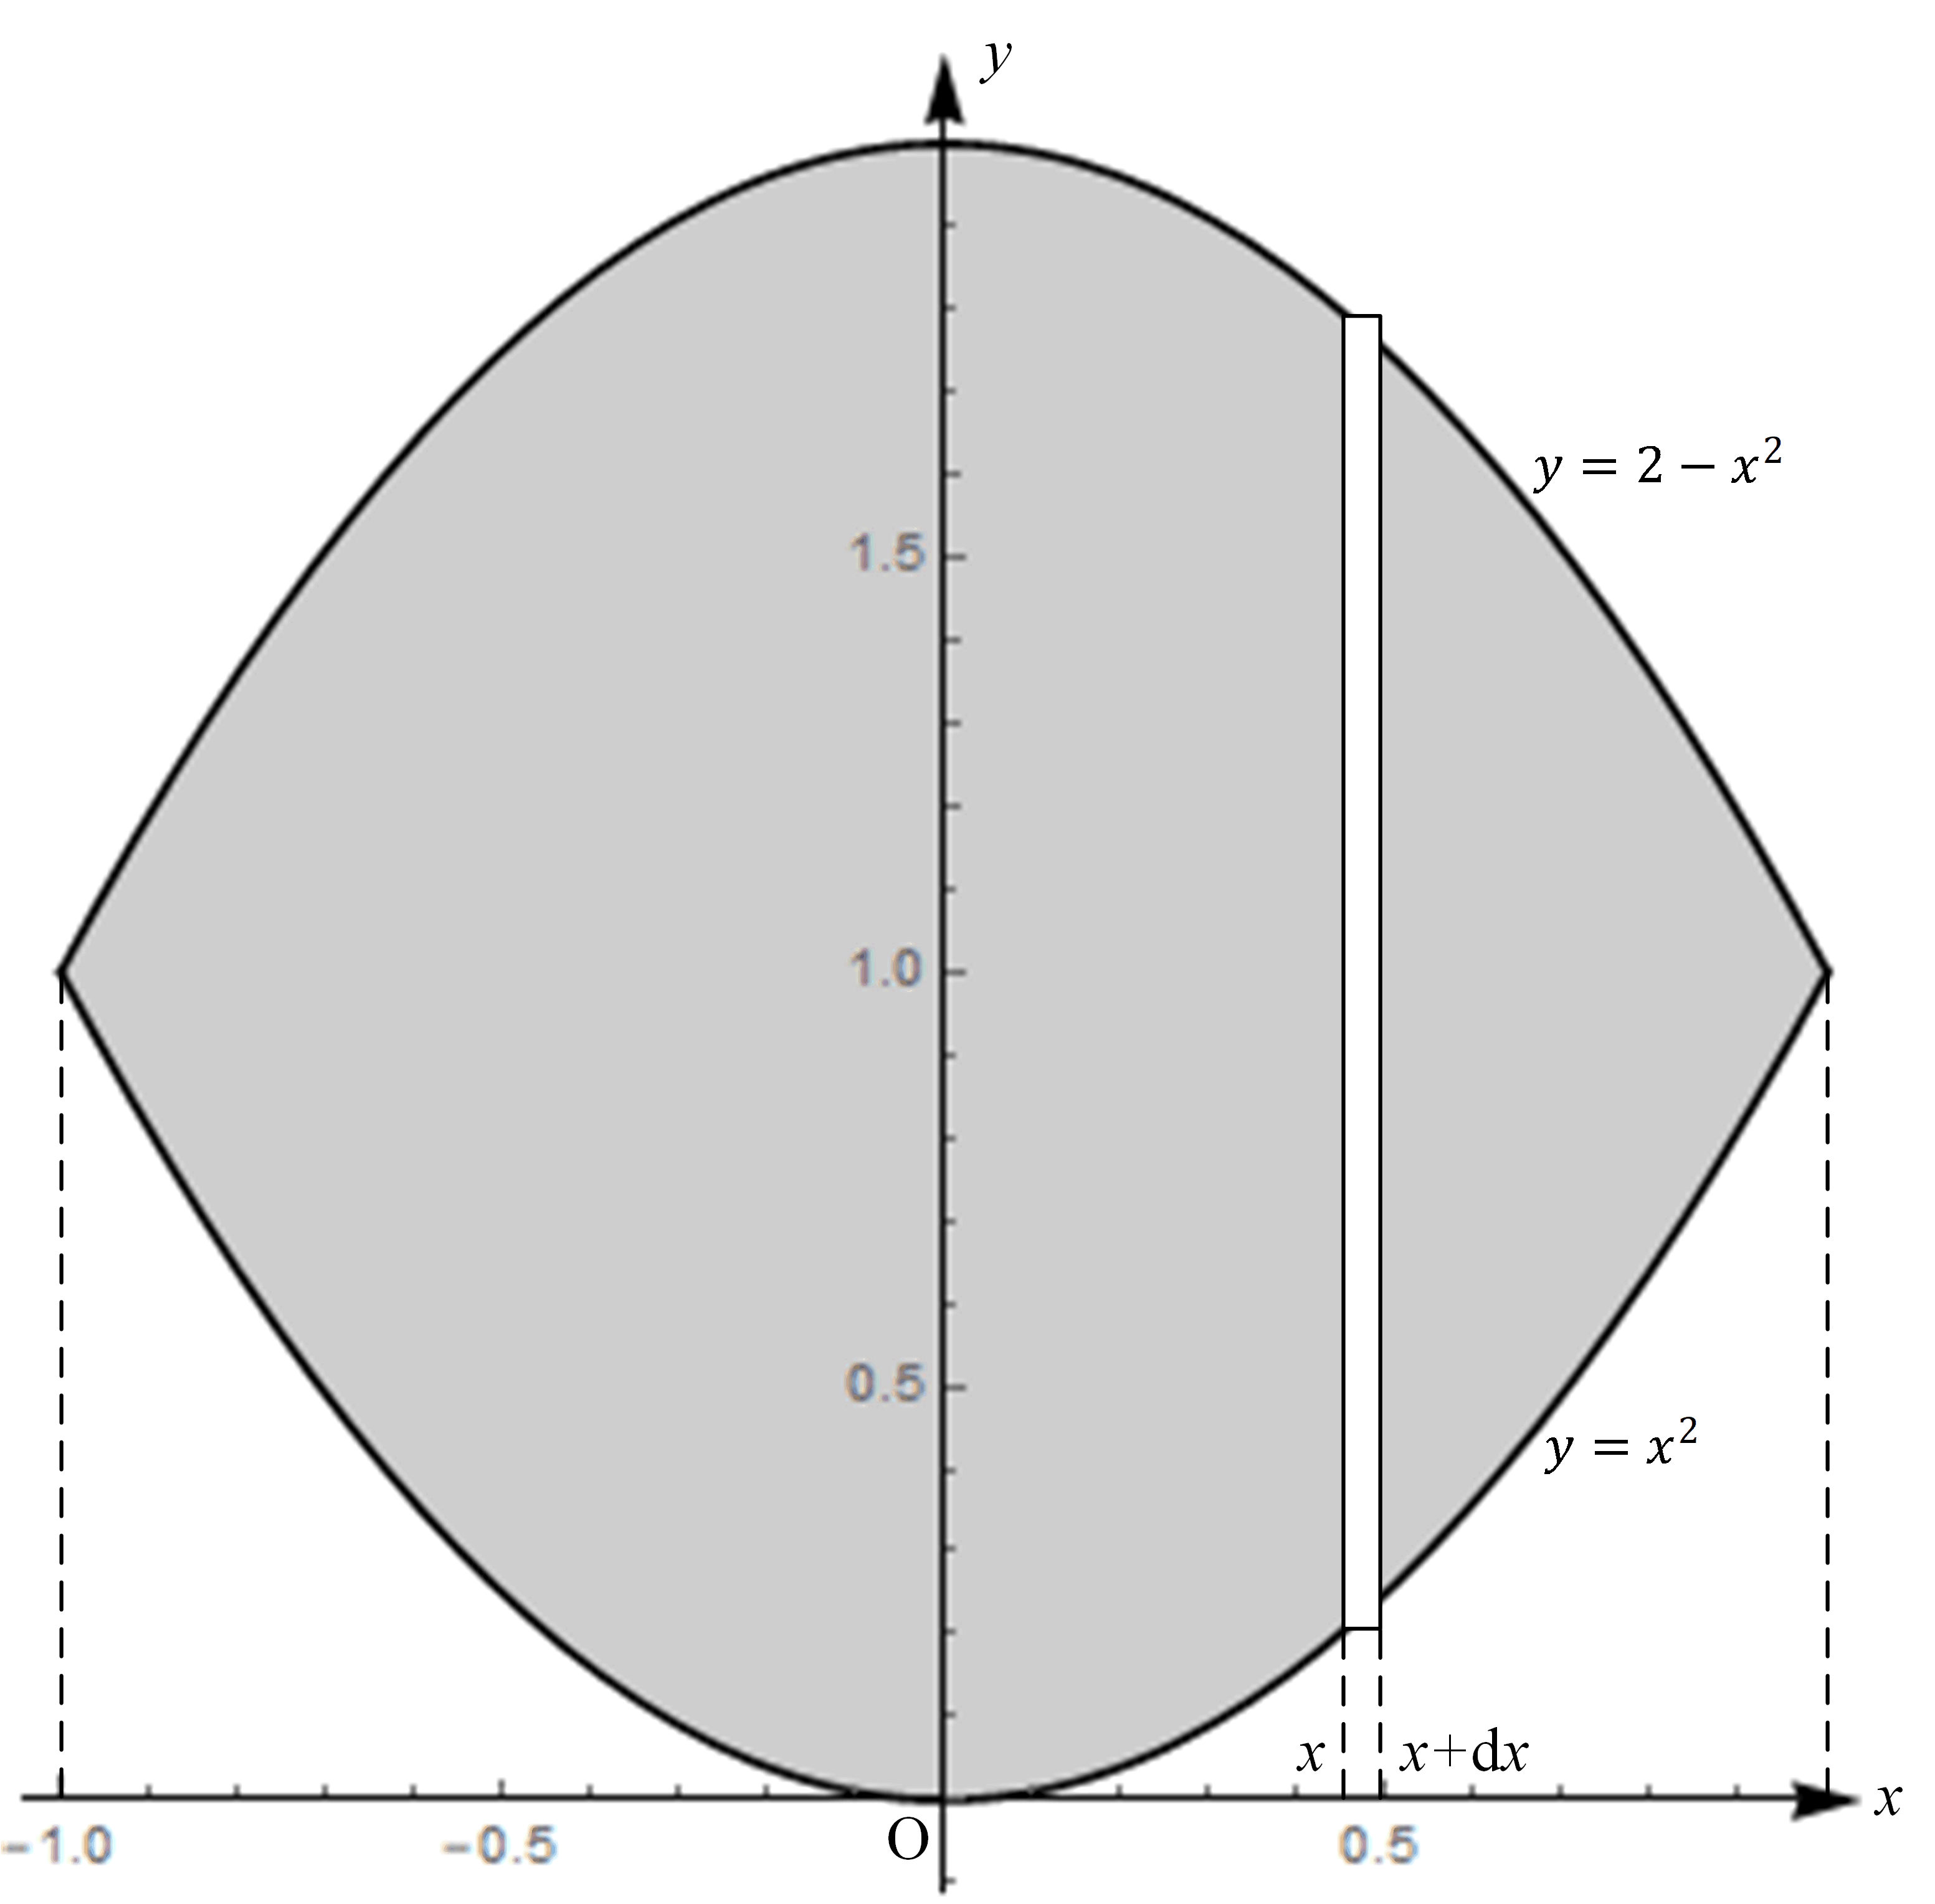
\includegraphics[height=0.3\textheight]{F:/life/2018AutumnTA/Exercises/11/Fig5-1-1.png}
\end{center}
\caption{习题7.5 1.(1)题图示}
\label{5-1-1}
\end{figure}
取图示面积元,图形面积
\[S=\int_{-1}^1(2-x^2-x^2)\mathrm dx=\int_{-1}^1(2-2x^2)\mathrm dx=2x-\frac23x^3\Big|_{-1}^1=4-\frac43=\frac83.\]
(2)各曲线围成的图形如图~\ref{5-1-2}所示,
\begin{figure}[H]
\begin{center}
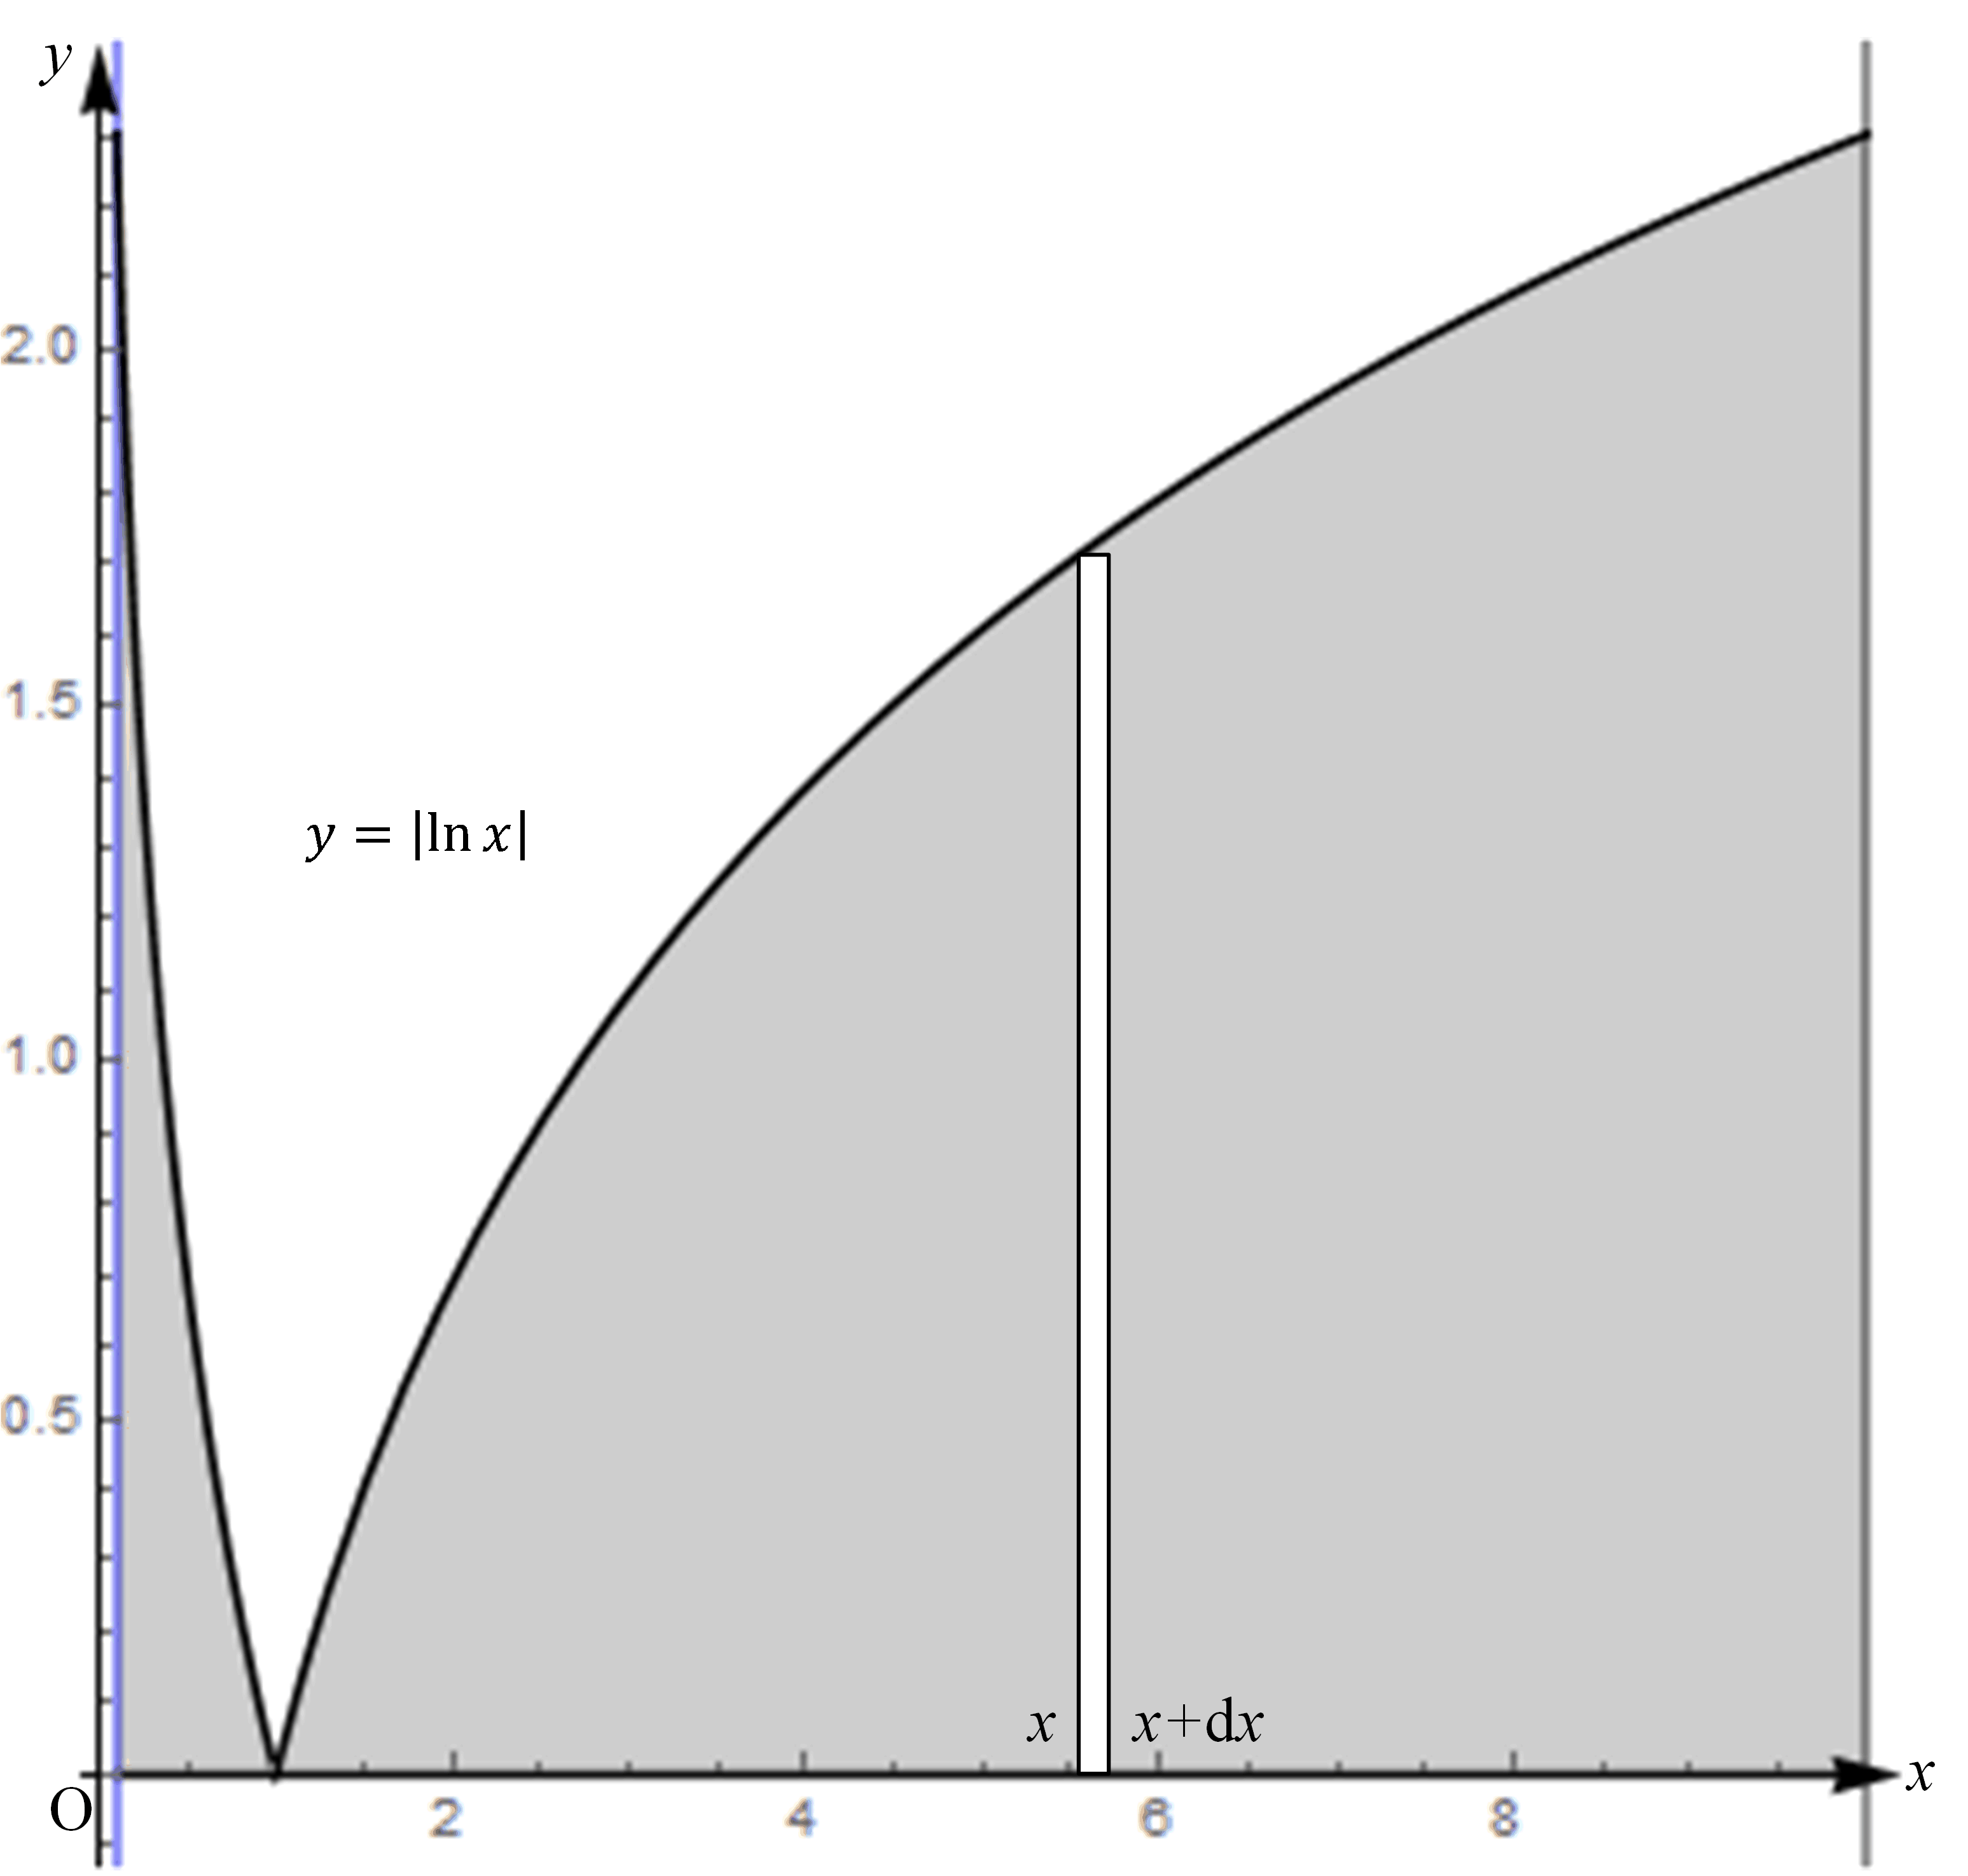
\includegraphics[height=0.3\textheight]{F:/life/2018AutumnTA/Exercises/11/Fig5-1-2.png}
\end{center}
\caption{习题7.5 1.(2)题图示}
\label{5-1-2}
\end{figure}
取图示面积元,图形面积
\[\begin{split}
S&=\int_{\frac1{10}}^{10}|\ln x|\mathrm dx=-\int_{\frac1{10}}^1\ln x\mathrm dx+\int_1^{10}\ln x\mathrm dx=-(x\ln x-x)\Big|_{\frac1{10}}^1+(x\ln x-x)\Big|_1^{10}\\
&=1+(\frac1{10}\ln\frac1{10}-\frac1{10})+10\ln10-10-(-1)=-\frac{81}{10}+\frac{99}{10}\ln10.
\end{split}\]
(3)该曲线围成的图形如图~\ref{5-1-3}所示,
\begin{figure}[H]
\begin{center}
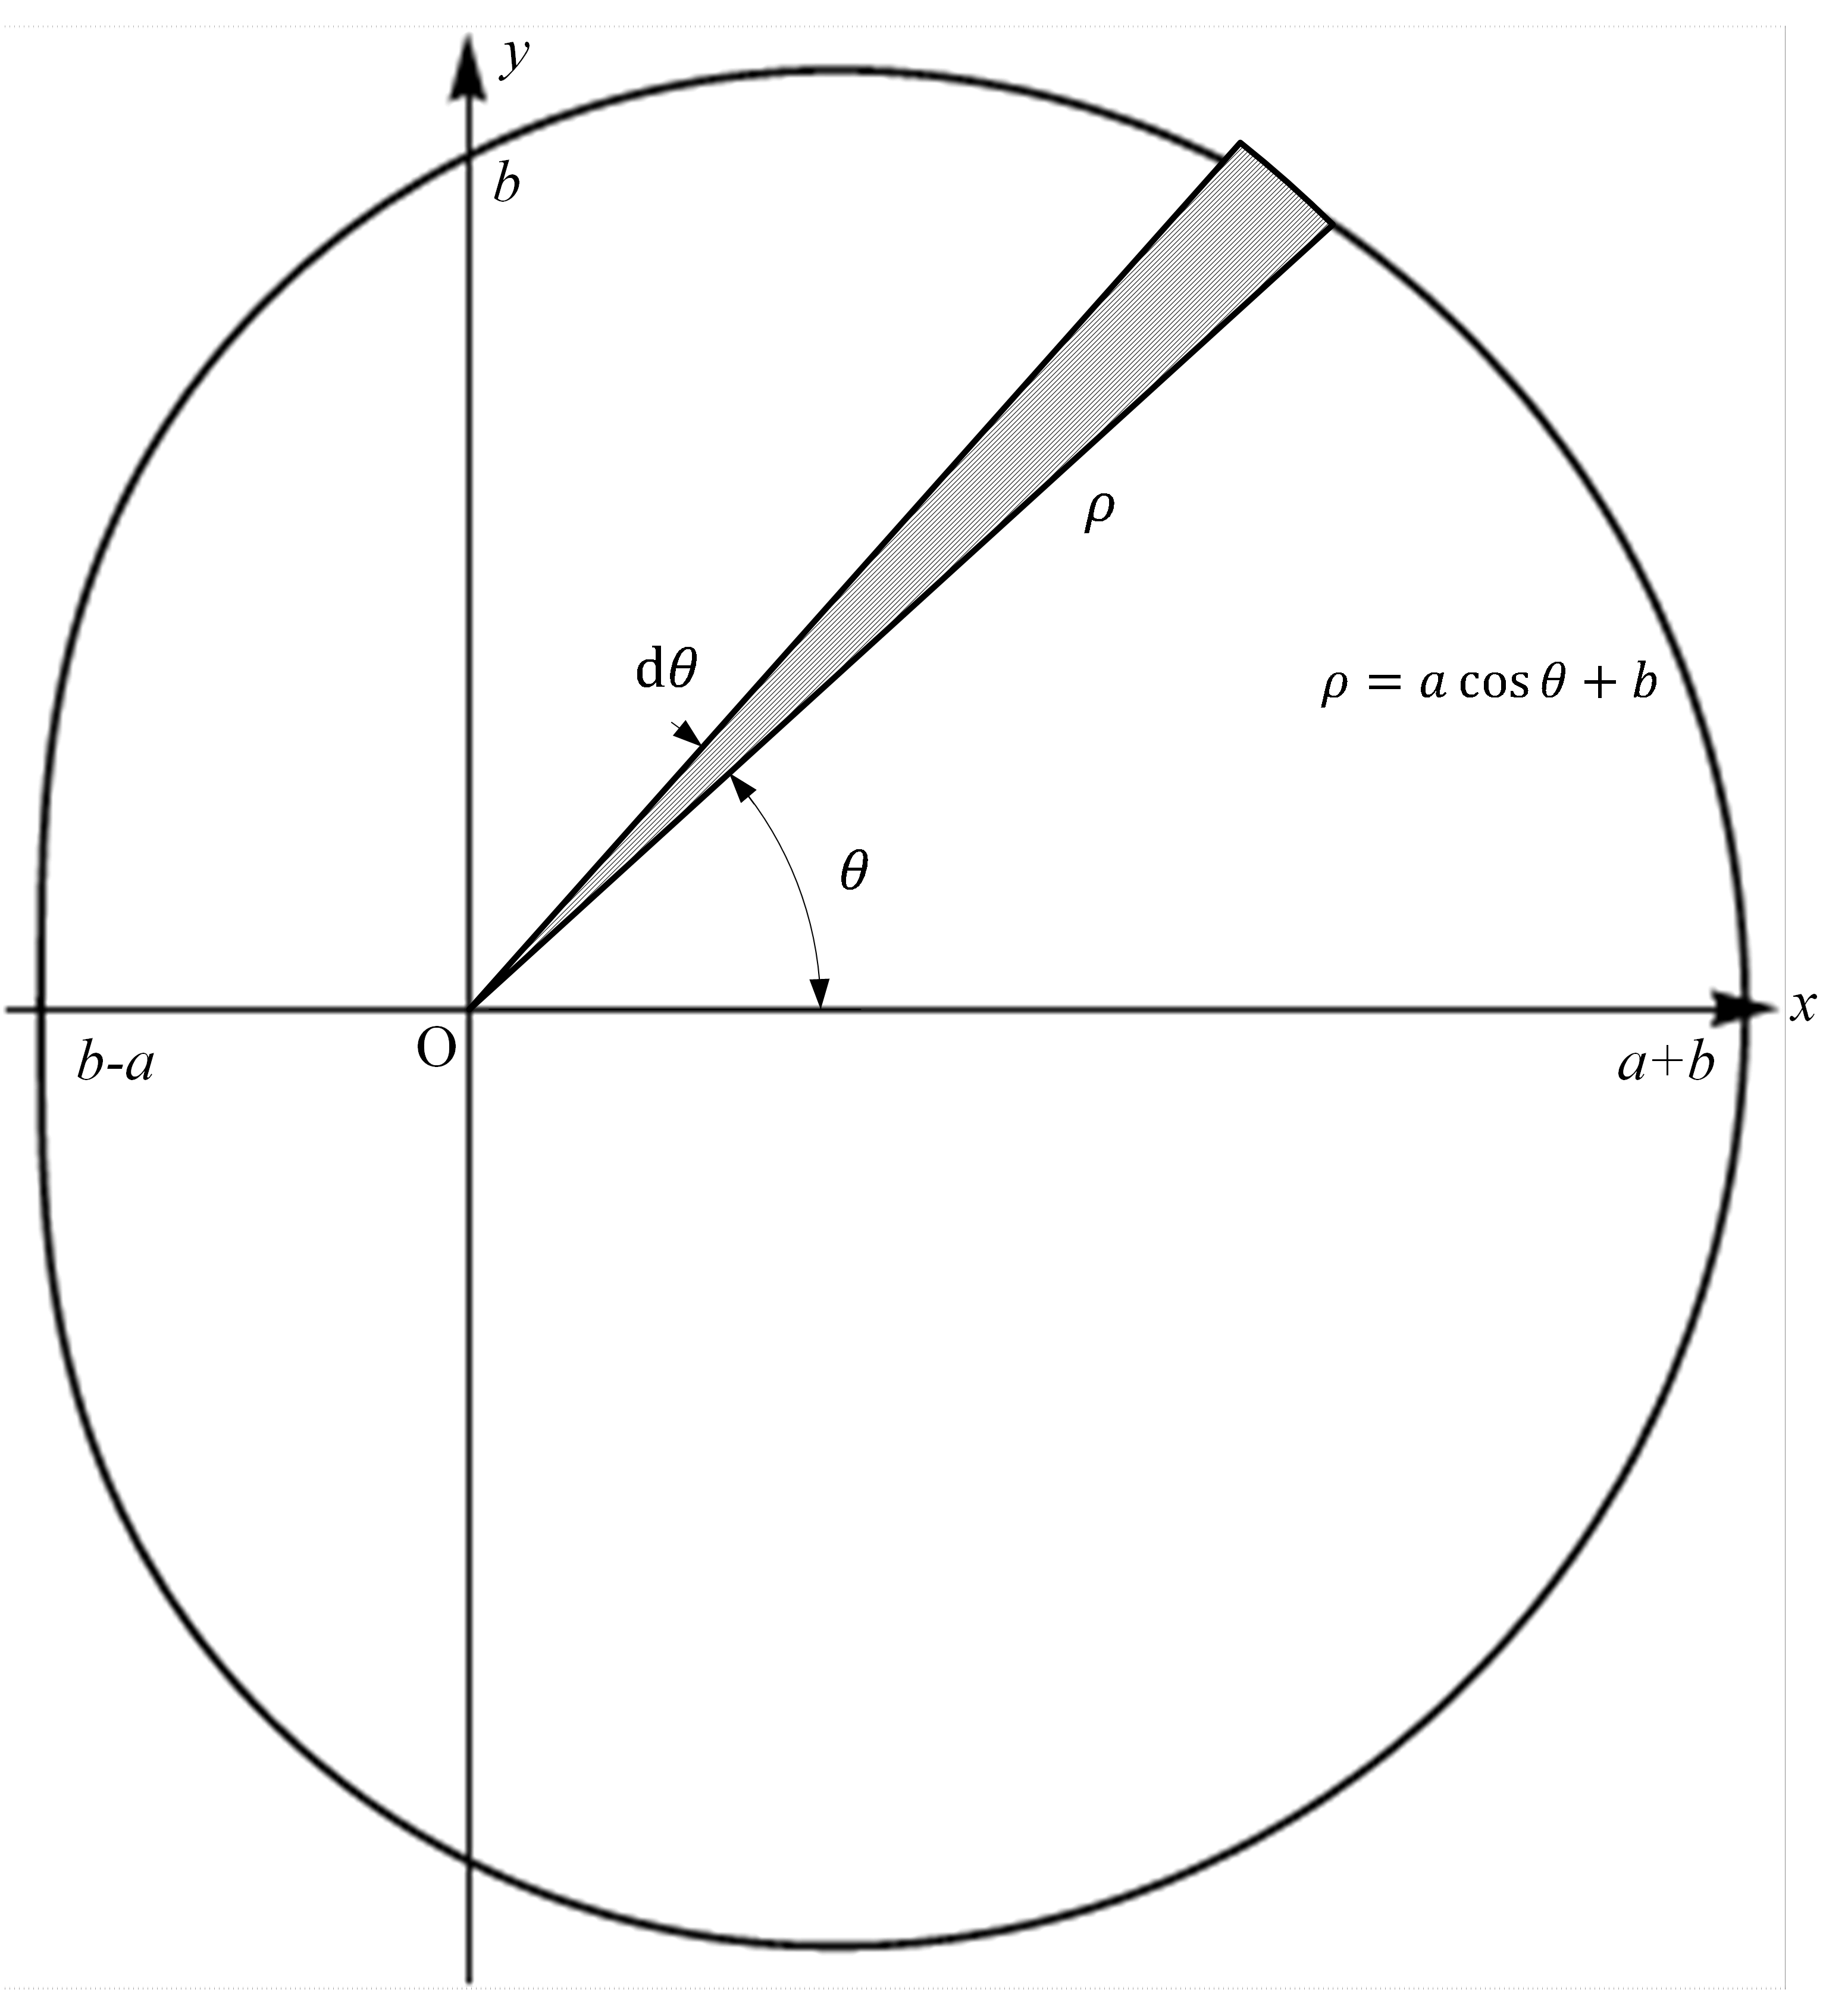
\includegraphics[height=0.35\textheight]{F:/life/2018AutumnTA/Exercises/11/Fig5-1-3.png}
\end{center}
\caption{习题7.5 1.(3)题图示}
\label{5-1-3}
\end{figure}
取图示面积元,图形面积
\[\begin{split}
S&=\int_0^{2\pi}\frac12\rho^2\mathrm d\theta=\int_0^{2\pi}\frac12(a\cos\theta+b)^2\mathrm d\theta=\frac12\int_0^{2\pi}(a^2\cos^2\theta+2ab\cos\theta+b^2)\mathrm d\theta\\
&=\frac12\int_0^{2\pi}[\frac{a^2}2(1+\cos2\theta)+2ab\cos\theta+b^2]\mathrm d\theta=\frac12[\frac12a^2(\theta+\frac12\sin2\theta)+2ab\sin\theta+b^2\theta]_0^{2\pi}\\
&=\frac12[\frac12a^2(2\pi+0)+b^22\pi]=\frac\pi2a^2+\pi b^2.
\end{split}\]
(4)该曲线围成的图形如图~\ref{5-1-4}所示,
\begin{figure}[H]
\begin{center}
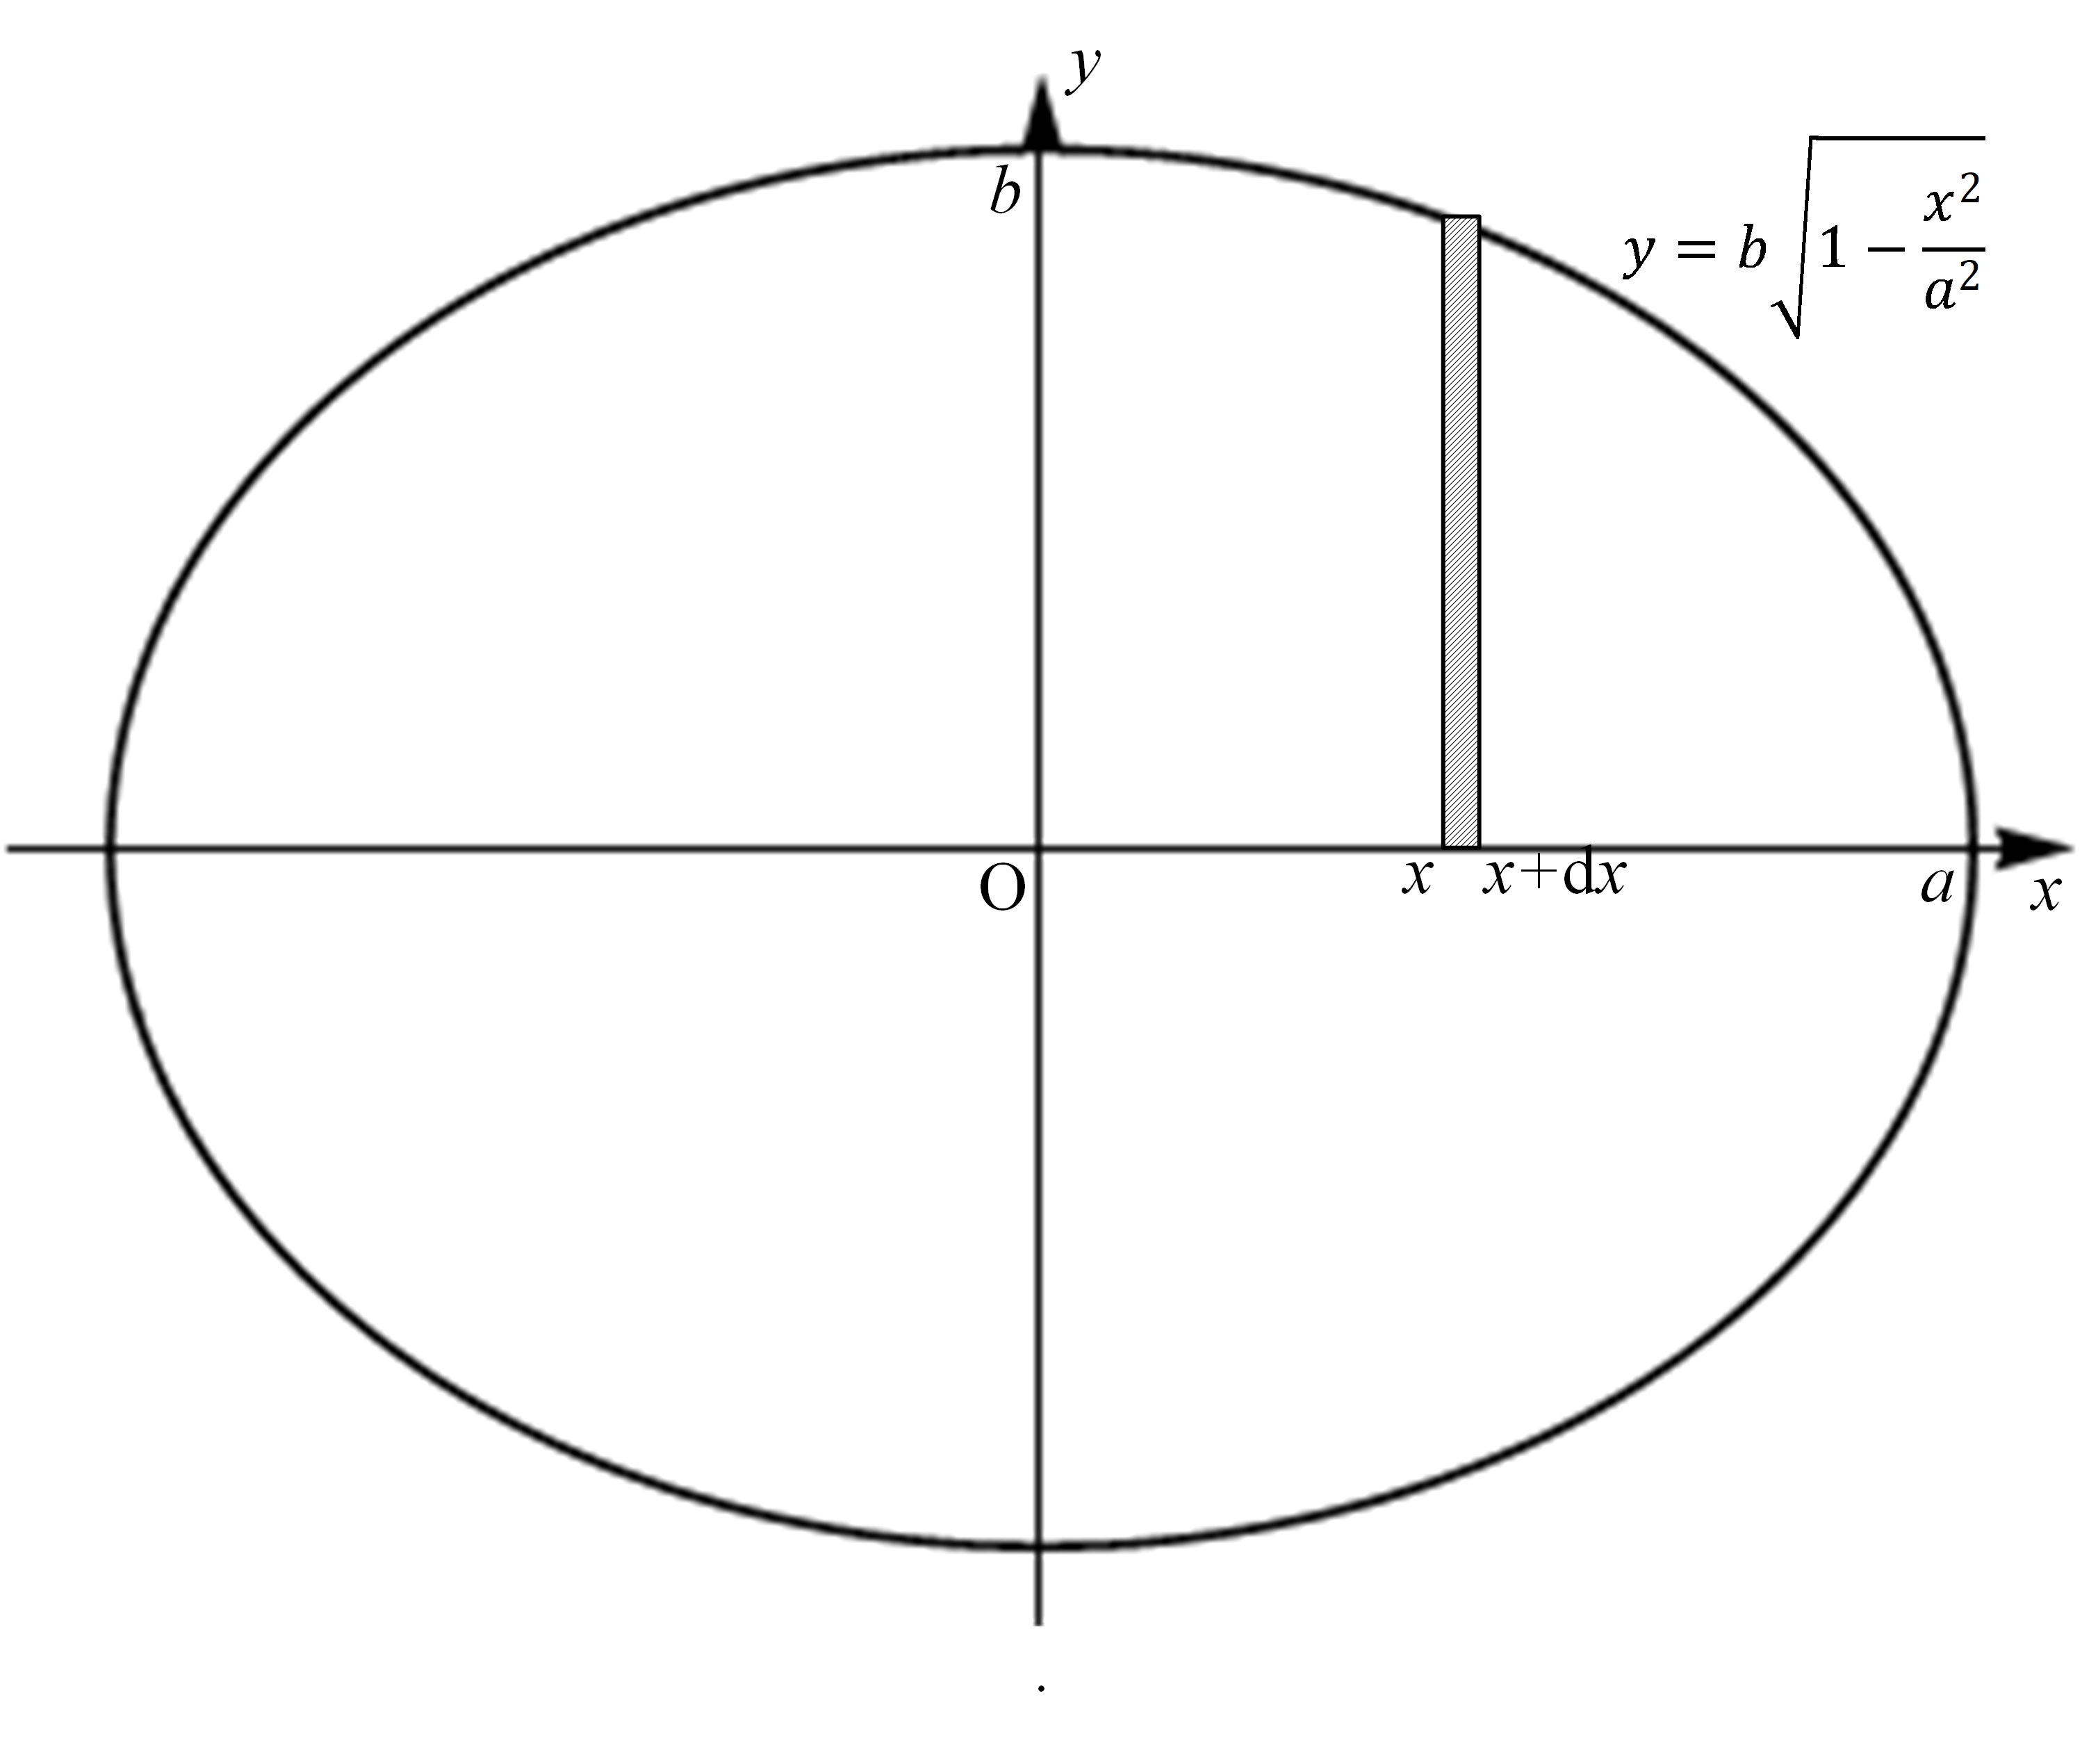
\includegraphics[height=0.25\textheight]{F:/life/2018AutumnTA/Exercises/11/Fig5-1-4.png}
\end{center}
\caption{习题7.5 1.(4)题图示}
\label{5-1-4}
\end{figure}
根据椭圆的对称性,其面积为第一象限部分面积的四倍,取图示面积元,图形面积
\[\begin{split}
S&=4\int_0^ab\sqrt{1-\frac{x^2}{a^2}}\mathrm dx=4\frac ba\int_0^a\sqrt{a^2-x^2}\mathrm dx=4\frac ba\int_0^{\frac\pi2}(a\cos t)(a\cos t)\mathrm dt\\
&=4\frac ba\int_0^{\frac\pi2}a^2\frac{1+\cos2t}2\mathrm dt=2ab\int_0^{\frac\pi2}(1+\cos2t)\mathrm dt=2ab(t+\frac12\sin2t)\Big|_0^\frac\pi2\\
&=\pi ab.
\end{split}\]
(5)由$\sqrt{\frac xa}+\sqrt{\frac yb}=1$知$0\leq x\leq a,0\leq y\leq b$,各曲线围成的图形如图~\ref{5-1-5}所示,
\begin{figure}[H]
\begin{center}
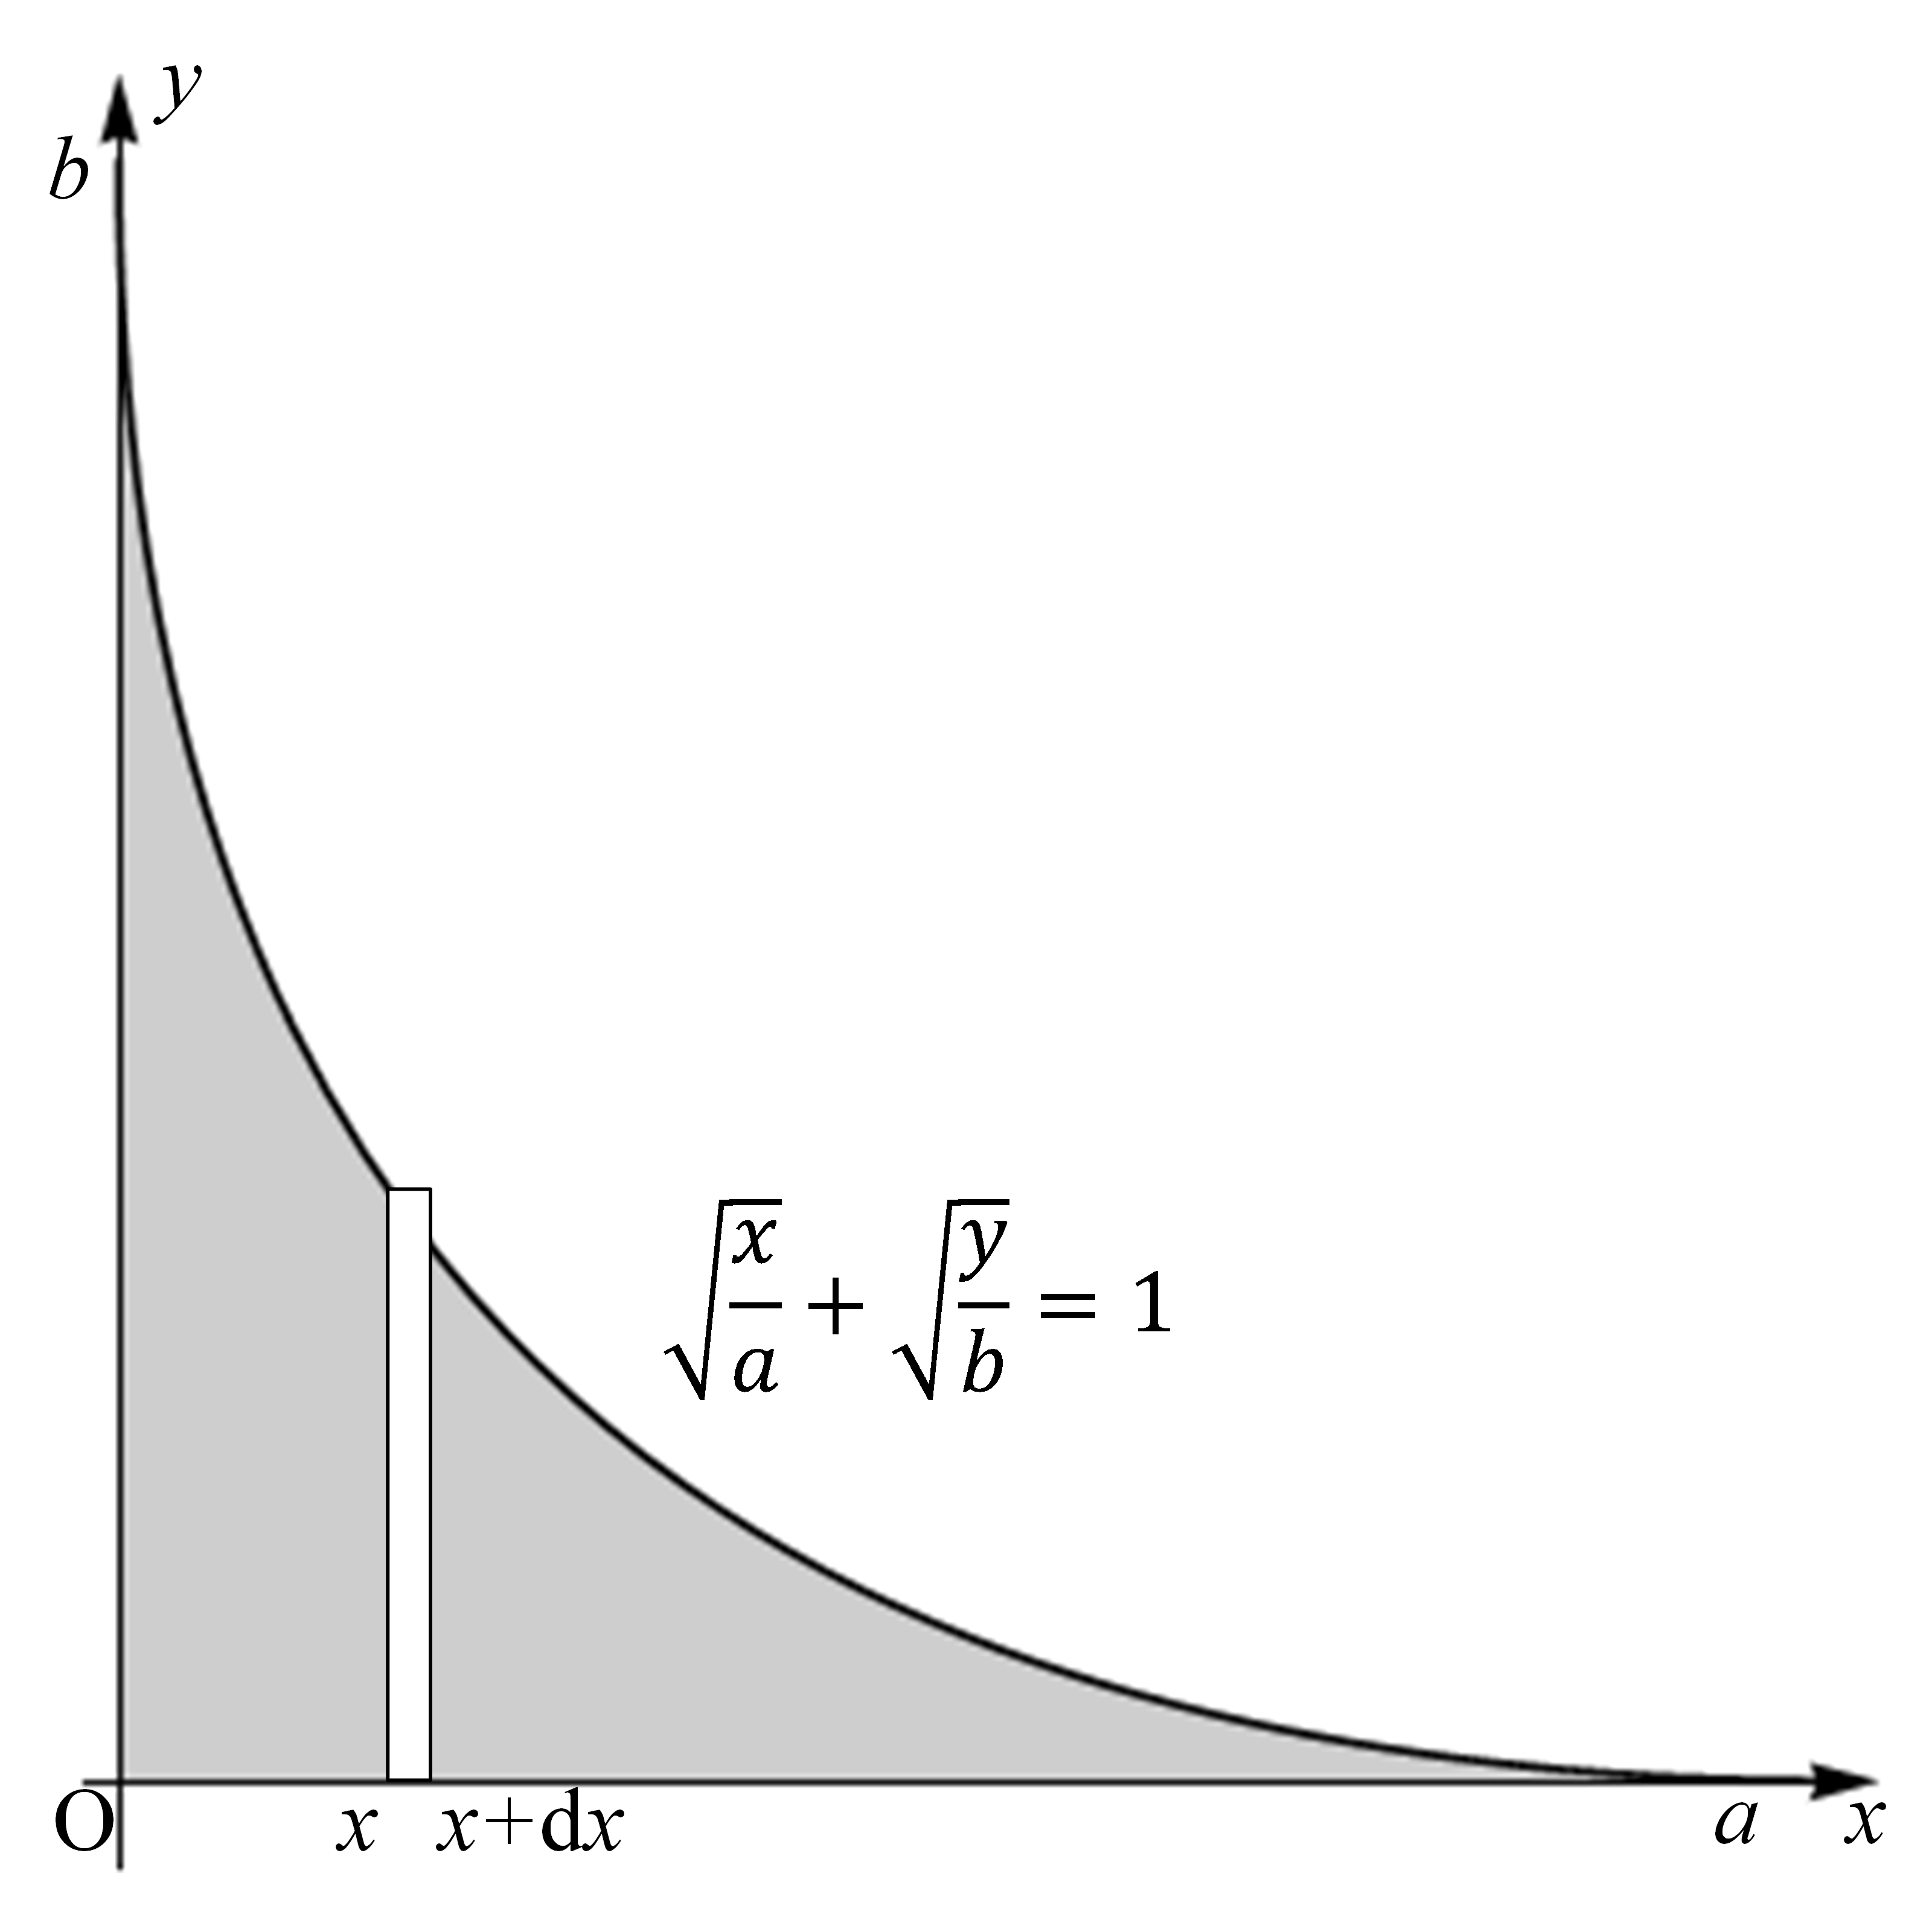
\includegraphics[height=0.3\textheight]{F:/life/2018AutumnTA/Exercises/11/Fig5-1-5.png}
\end{center}
\caption{习题7.5 1.(5)题图示}
\label{5-1-5}
\end{figure}
取图示面积元,图形面积
\[\begin{split}
S&=\int_0^ay\mathrm dx=\int_0^ab(1-\sqrt{\frac xa})^2\mathrm dx=b\int_0^a(1+\frac xa-2\sqrt{\frac xa})\mathrm dx=b[x+\frac 1{2a}x^2-\frac2{\sqrt a}\frac23(\sqrt x)^3]_0^a\\
&=b(a+\frac12a-\frac43a)=\frac16ab.
\end{split}\]
\item求下列曲线的弧长:
\newline
(1)$y=x\sqrt x,0\leq x\leq4$;
\newline
(2)$\sqrt x+\sqrt y=1$;
\newline
(3)圆的渐开线$\begin{cases}
x=a(\cos t+t\sin t),\\
y=a(\sin t-t\cos t),
\end{cases}t\in[0,2\pi]$;
\newline
(4)心脏线$\rho=a(1+\cos\theta),\theta\in[0,2\pi]$.

解:(1)曲线如图~\ref{5-2-1}所示,
\begin{figure}[H]
\begin{center}
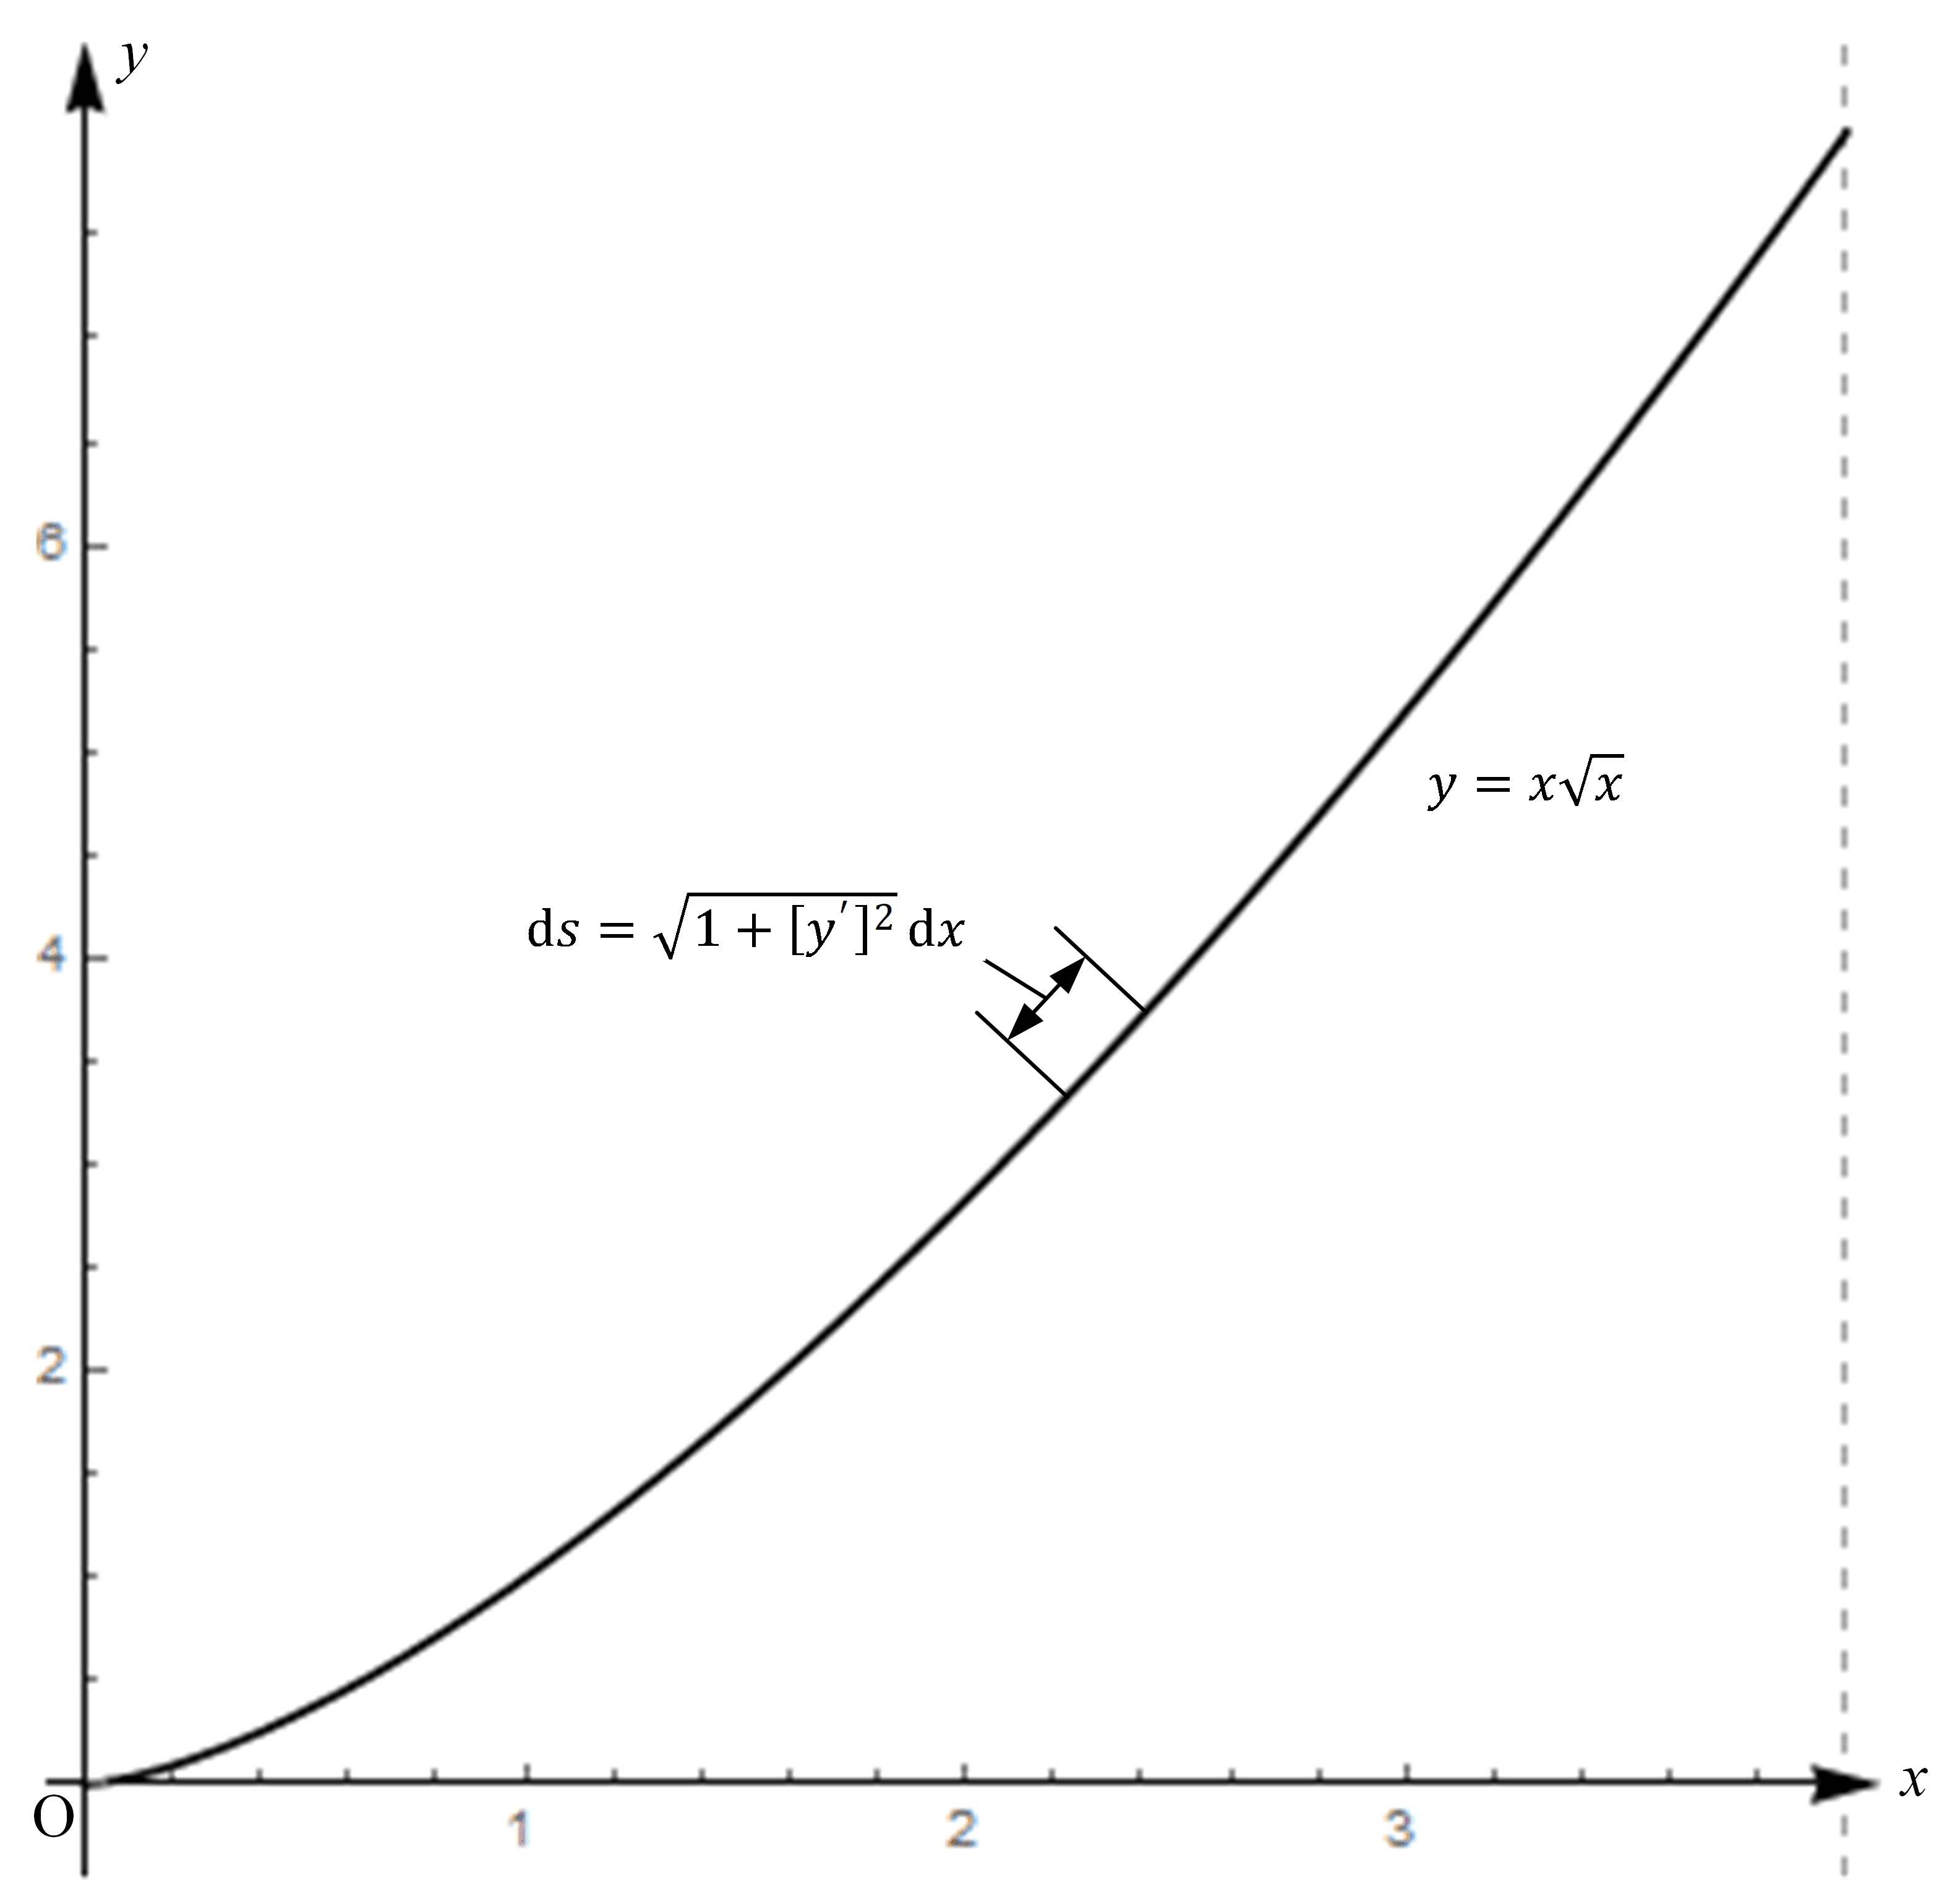
\includegraphics[height=0.4\textheight]{F:/life/2018AutumnTA/Exercises/11/Fig5-2-1.png}
\end{center}
\caption{习题7.5 2.(1)题图示}
\label{5-2-1}
\end{figure}
取图示弧段,曲线长度
\[\begin{split}
l&=\int_0^4\sqrt{1+(y')^2}\mathrm dx=\int_0^4\sqrt{1+(\frac32x^{\frac12})}\mathrm dx=\int_0^4\sqrt{1+\frac94x}\mathrm dx\\
&=\frac49\int_0^4\sqrt{1+\frac94x}\mathrm d(1+\frac94)=\frac49\frac23(1+\frac94x)^{\frac32}\Big|_0^4=\frac8{27}[(1+9)^\frac32-1]=\frac8{27}(10^{\frac32}-1).
\end{split}\]
(2)由$\sqrt x+\sqrt y=1$知$0\leq x\leq1,0\leq y\leq1$,曲线如图~\ref{5-2-2}所示,
\begin{figure}[H]
\begin{center}
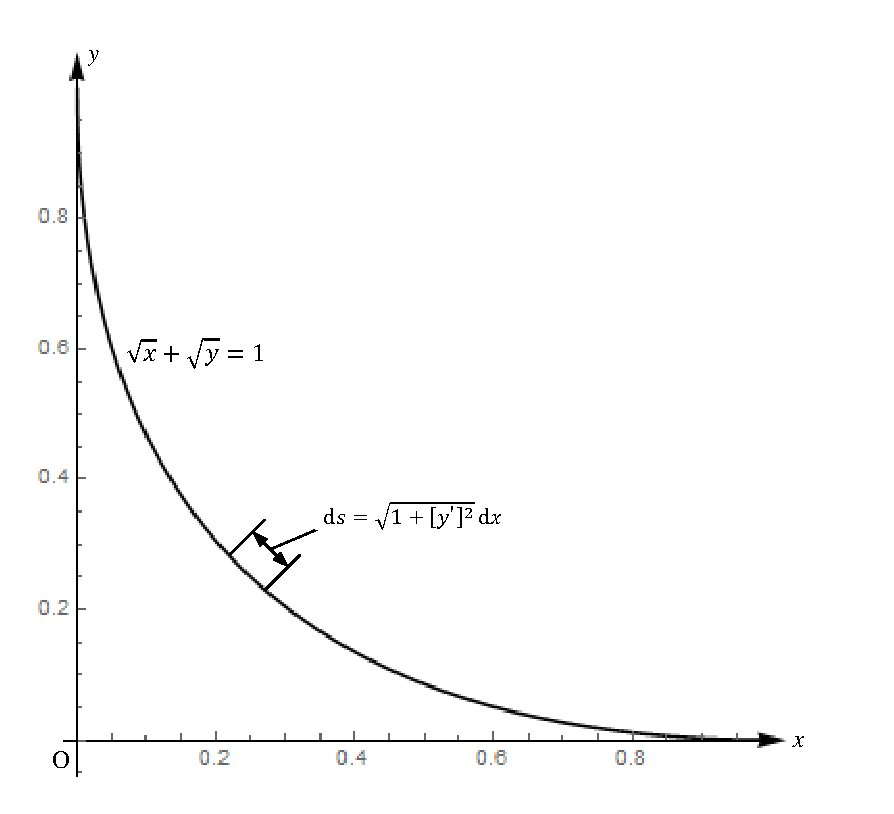
\includegraphics[height=0.4\textheight]{F:/life/2018AutumnTA/Exercises/11/Fig5-2-2.pdf}
\end{center}
\caption{习题7.5 2.(2)题图示}
\label{5-2-2}
\end{figure}
取图示弧段,曲线长度
\[\begin{split}
l&=\int_0^1\sqrt{1+(y')^2}\mathrm dx=\int_0^1\sqrt{1+[2(1-\sqrt x)\frac{-1}{2\sqrt x}]^2}\mathrm dx=\int_0^1\sqrt{1+(\frac{-1}{\sqrt x}+1)^2}\\
&=\int_0^1\sqrt{2+\frac1x-\frac2{\sqrt x}}\mathrm dx\xlongequal{t=\sqrt x}\int_0^1\sqrt{2-\frac2t+\frac1{t^2}}2t\mathrm dt=2\int_0^1\sqrt{2t^2-2t+1}\mathrm dt\\
&=\sqrt2\int_0^1\sqrt{4(t-\frac12)^2+1}\mathrm dt\xlongequal{2(t-\frac12)=\tan u}\sqrt2\int_{-\frac\pi4}^{\frac\pi4}(\sec u)\cdot\frac12\sec^2u\mathrm du=\frac{\sqrt2}2\int_{-\frac\pi4}^{\frac\pi4}\sec^3u\mathrm du\\
&=\frac{\sqrt2}2[\sec u\tan u\Big|_{-\frac\pi4}^{\frac\pi4}-\int_{-\frac\pi4}^{\frac\pi4}\tan u\tan \sec u\mathrm du]=2-\frac{\sqrt2}2\int_{-\frac\pi4}^{\frac\pi4}(\sec^2u-1)\sec u\mathrm du\\
&=2-\frac{\sqrt2}2\int_{-\frac\pi4}^{\frac\pi4}(\sec^3u-\sec u)\mathrm du=\frac12(2+\frac{\sqrt2}2\int_{-\frac\pi4}^{\frac\pi4}\sec u\mathrm du)=\frac12[2+\frac{\sqrt 2}2\ln(\sec u+\tan u)\Big|_{-\frac\pi4}^{\frac\pi4}]\\
&=\frac12\{2+\frac{\sqrt2}2[\ln(\sqrt 2+1)-\ln{\sqrt 2-1}]\}=1+\frac{\sqrt2}4\ln\frac{\sqrt2+1}{\sqrt2-1}=1+\frac{\sqrt2}2\ln(\sqrt2+1).
\end{split}\]
(3)曲线如图~\ref{5-2-3}所示,
\begin{figure}[H]
\begin{center}
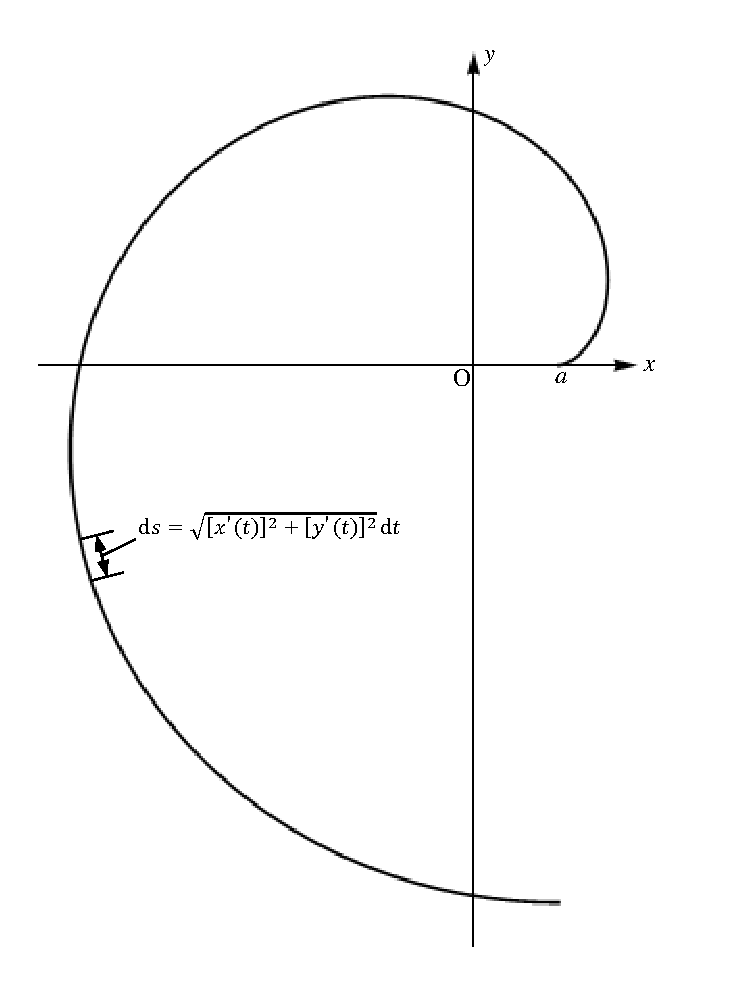
\includegraphics[height=0.5\textheight]{F:/life/2018AutumnTA/Exercises/11/Fig5-2-3.pdf}
\end{center}
\caption{习题7.5 2.(3)题图示}
\label{5-2-3}
\end{figure}
取图示弧段,曲线长度
\[l=\int_0^{2\pi}\sqrt{[x'(t)]^2+[y'(t)]^2}\mathrm dt=\int_0^{2\pi}\sqrt{a^2(t\cos t)^2+a^2(t\sin t)^2}\mathrm dt=a\int_0^{2\pi}t\mathrm dt=\frac a2t^2\Big|_0^{2\pi}
=2a\pi^2.\]
(4)曲线如图~\ref{5-2-4}所示,
\begin{figure}[H]
\begin{center}
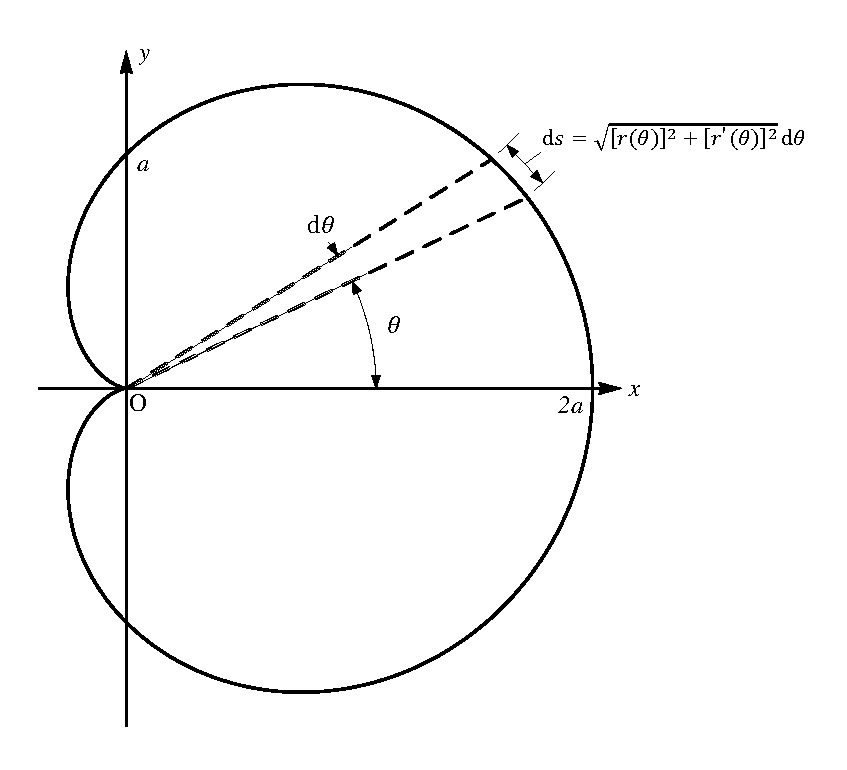
\includegraphics[height=0.4\textheight]{F:/life/2018AutumnTA/Exercises/11/Fig5-2-4.pdf}
\end{center}
\caption{习题7.5 2.(4)题图示}
\label{5-2-4}
\end{figure}
取图示弧段,曲线长度
\[\begin{split}
l&=\int_0^{2\pi}\sqrt{[r(\theta)]^2+[r'(\theta)]^2}\mathrm d\theta=\int_0^{2\pi}\sqrt{a^2(1+\cos\theta)^2+a^2(-\sin\theta)^2}\mathrm d\theta\\
&=a\int_0^{2\pi}\sqrt{(1+\cos\theta)^2+(-\sin\theta)^2}\mathrm d\theta=a\int_0^{2\pi}\sqrt{2+2\cos\theta}\mathrm d\theta\\
&=a\int_0^{2\pi}\sqrt{4\cos^2\frac\theta2}\mathrm d\theta=2a\int_0^{2\pi}|\cos\frac\theta2|\mathrm d\theta\\
&=2a(\int_{0}^{\pi}\cos\frac\theta2\mathrm d\theta-\int_{\pi}^{2\pi}\cos\frac\theta2\mathrm d\theta)\\
&=4a\int_{0}^{\pi}\cos\frac\theta2\mathrm d\theta=8a\sin\frac\theta2\Big|_0^\pi=8a.
\end{split}\]
\item求下列曲线的曲率及曲率半径:
\newline
(1)抛物线$y^2=2px,p>0$;
\newline
(2)旋轮线$\begin{cases}
x=a(t-\sin t),\\
y=a(1-\cos t),
\end{cases},a>0$;
\newline
(3)双纽线$\rho^2=2a^2\cos2\theta,a>0$.

解:(1)如图~\ref{5-3-1}所示,
\begin{figure}[H]
\begin{center}
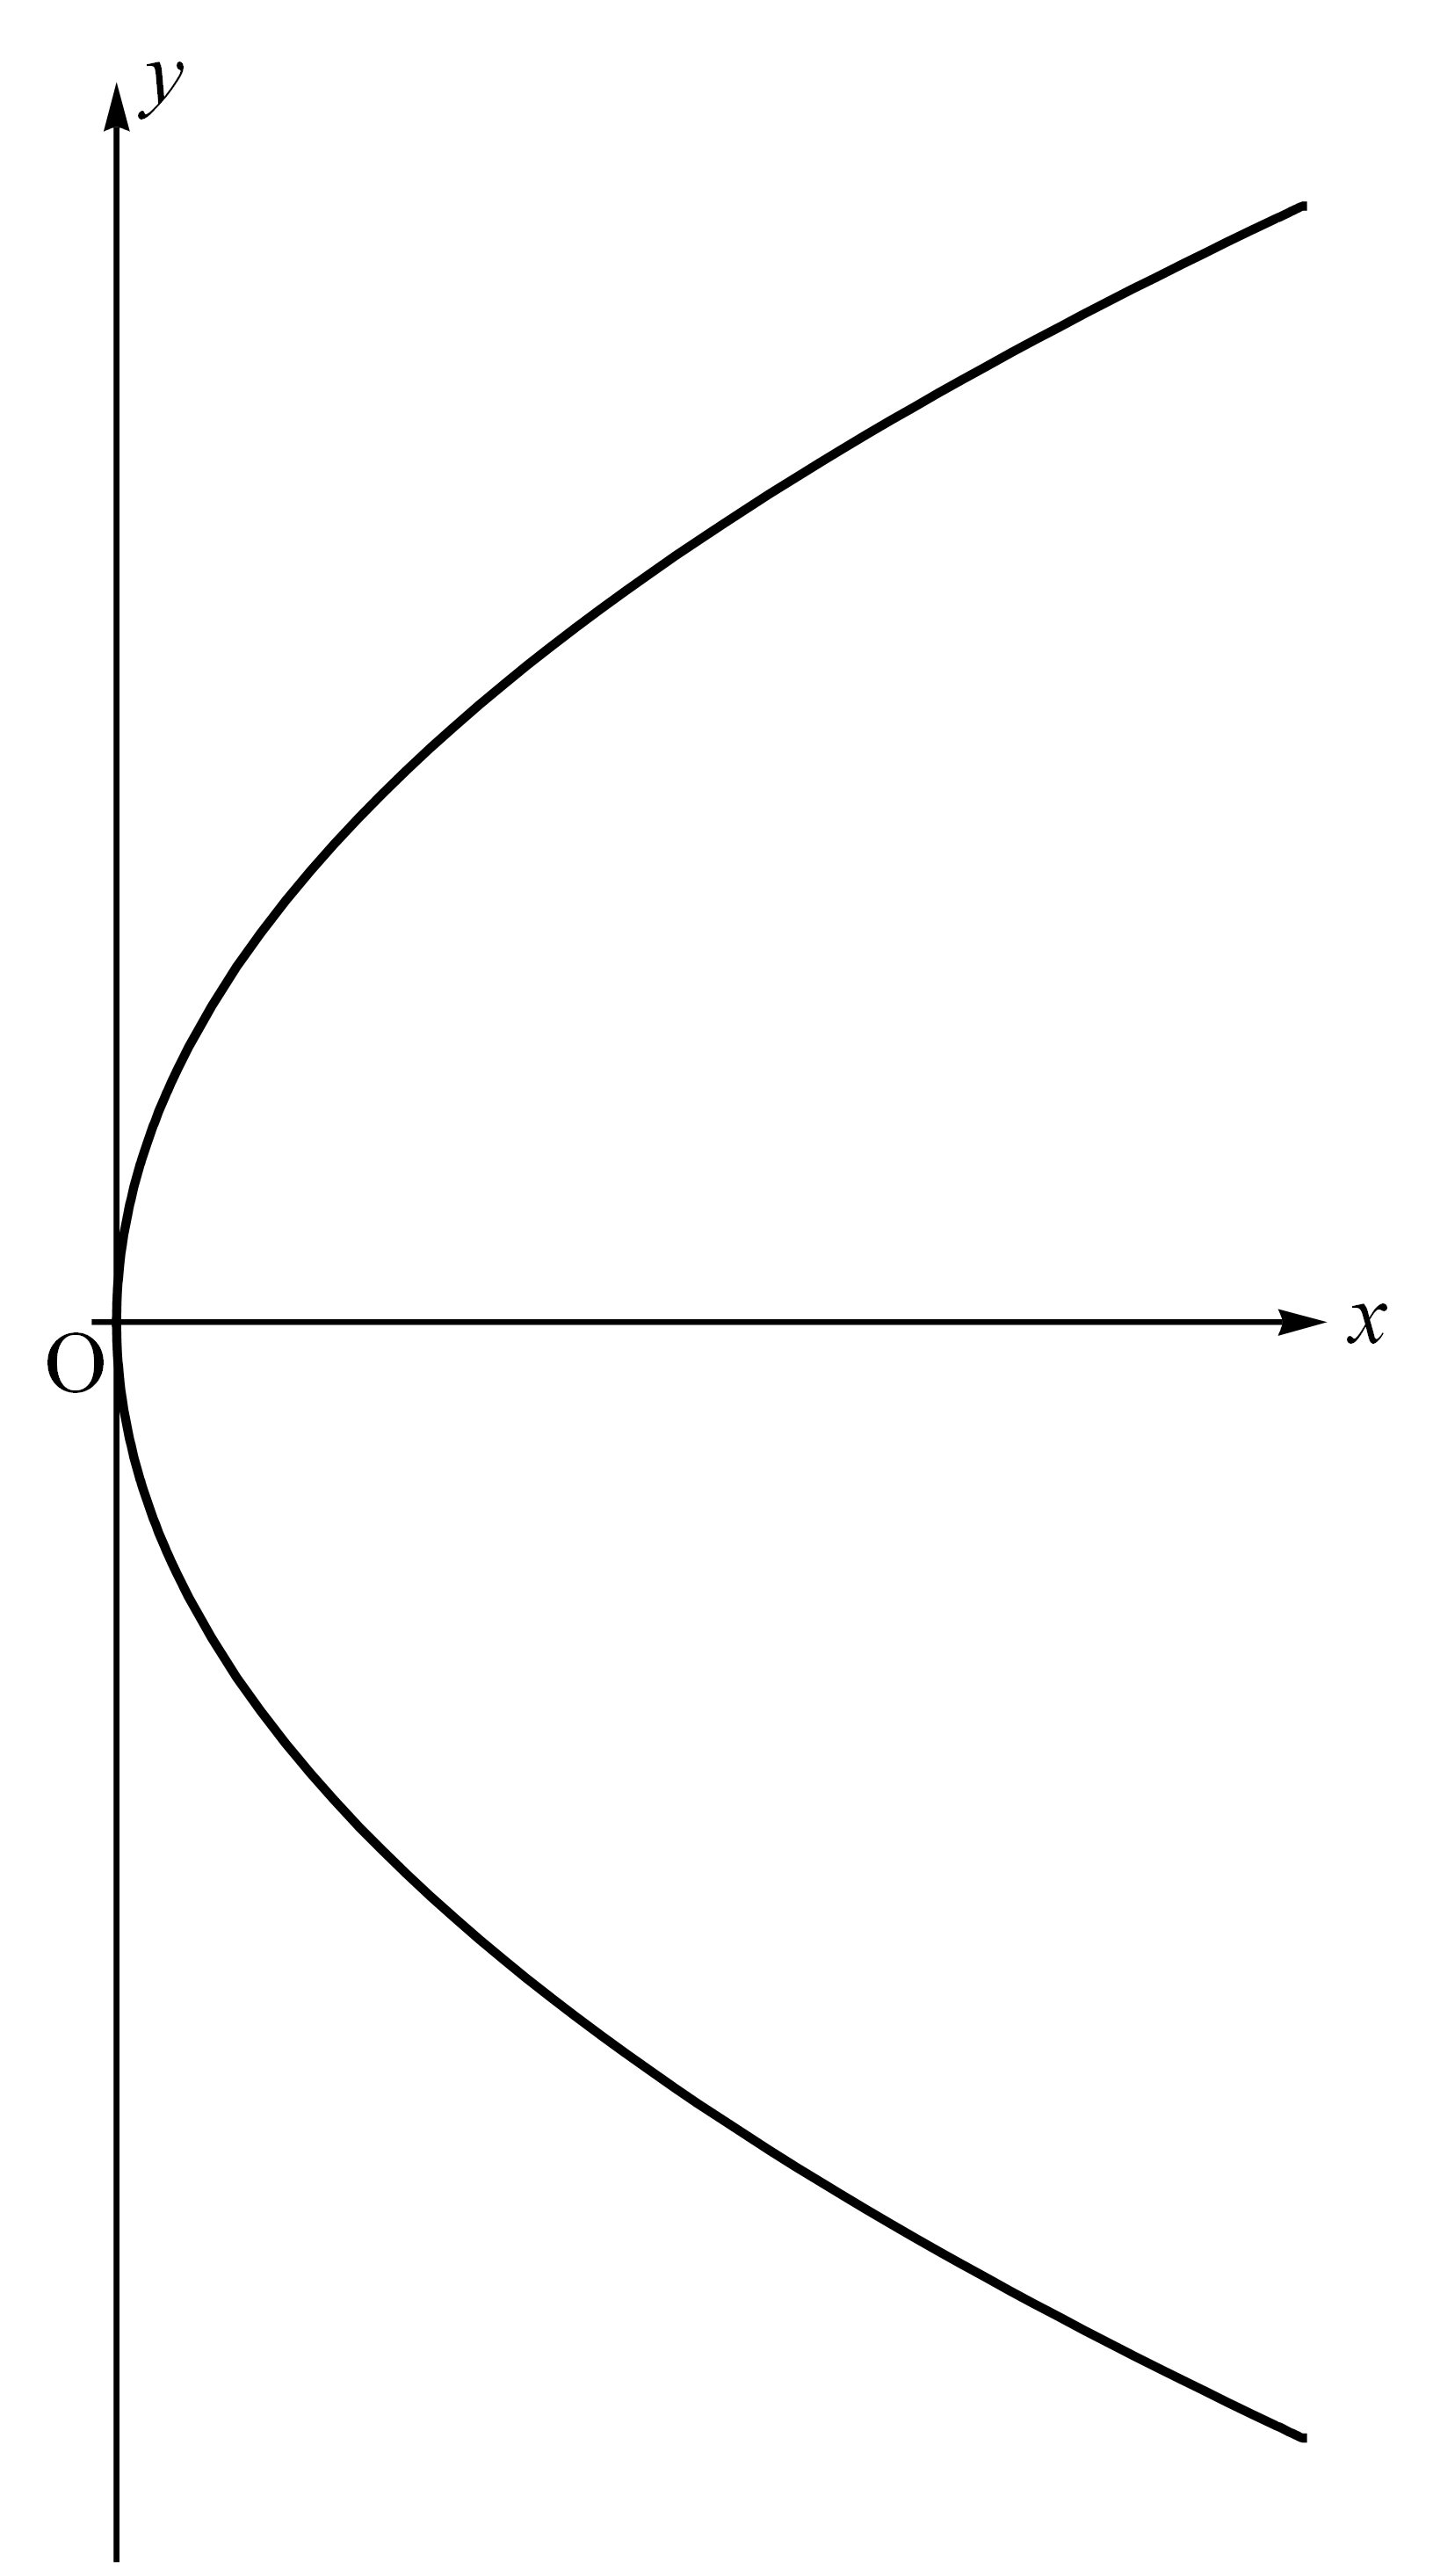
\includegraphics[height=0.4\textheight]{F:/life/2018AutumnTA/Exercises/11/Fig5-3-1.png}
\end{center}
\caption{习题7.5 3.(1)题图示}
\label{5-3-1}
\end{figure}
将$y^2=2px$两边对$x$求导得$2yy'=2p$,故$y'=\frac{p}y$

$\therefore y''=\frac{-py'}{y^2}=-\frac{p^2}{y^3}$

$\therefore$曲率$k=\frac{|y''|}{[1+(y')^2]^{\frac32}}=\frac{|-\frac{p^2}{y^3}|}{[1+(\frac{p}y)^2]^{\frac32}}=\frac{p^2}{(y^2+p^2)^{\frac32}}=\frac{p^2}{(2px+p^2)^{\frac32}}=\frac{\sqrt p}{(2x+p)^{\frac32}}$

曲率半径$R=\frac1k=\frac{(2x+p)^{\frac32}}{\sqrt p}$.

(2)如图~\ref{5-3-2}所示,
\begin{figure}[H]
\begin{center}
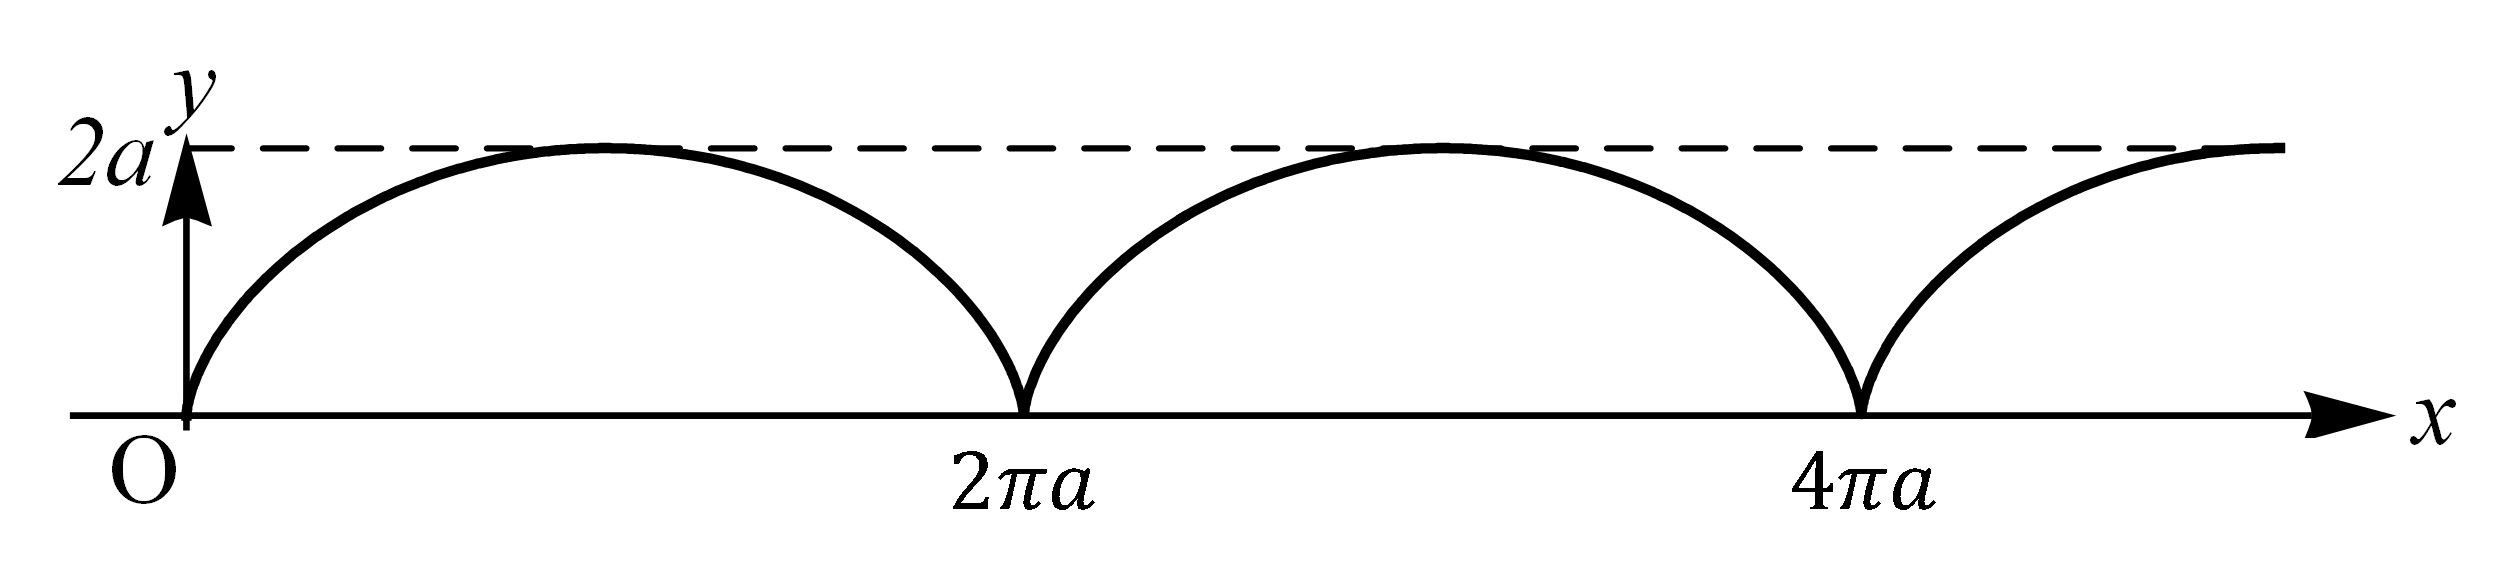
\includegraphics[height=0.1\textheight]{F:/life/2018AutumnTA/Exercises/11/Fig5-3-2.png}
\end{center}
\caption{习题7.5 3.(2)题图示}
\label{5-3-2}
\end{figure}
$x'(t)=a(1-\cos t),y'(t)=a\sin t$

$x''(t)=a\sin t,y''(t)=a\cos t$

$\therefore$曲率$k=\frac{|y''(t)x'(t)-y'(t)x''(t)|}{\{[x'(t)]^2+[y'(t)]^2\}^{\frac32}}=\frac{|a\cos t\cdot a(1-\cos t)-a\sin t\cdot a\sin t|}{\{[a(1-\cos t)]^2+[a\sin t]^2\}^{\frac32}}=\frac{|a^2\cos t-a^2|}{a^3(1-2\cos t+1)^{\frac32}}=\frac{|\cos t-1|}{a(2-2\cos t)^{\frac32}}\\
=\frac1{2\sqrt2a\sqrt{1-\cos t}}$

曲率半径$R=\frac1k=2\sqrt2a\sqrt{1-\cos t}$.

(3)由$\rho^2=2a^2\cos2\theta$得$\cos2\theta\geq0$,当$\theta$在$[0,2\pi)$内取值时,$0\leq2\theta\leq\frac\pi2\text{或}\frac32\pi\leq2\theta\leq\frac52\pi\text{或}\frac72\pi\leq2\theta<4\pi$,即$0\leq\theta\leq\frac\pi4\text{或}\frac34\pi\leq\theta\leq\frac54\pi\text{或}\frac74\pi\leq\theta<2\pi$,曲线形状如图~\ref{5-3-3}所示,
\begin{figure}[H]
\begin{center}
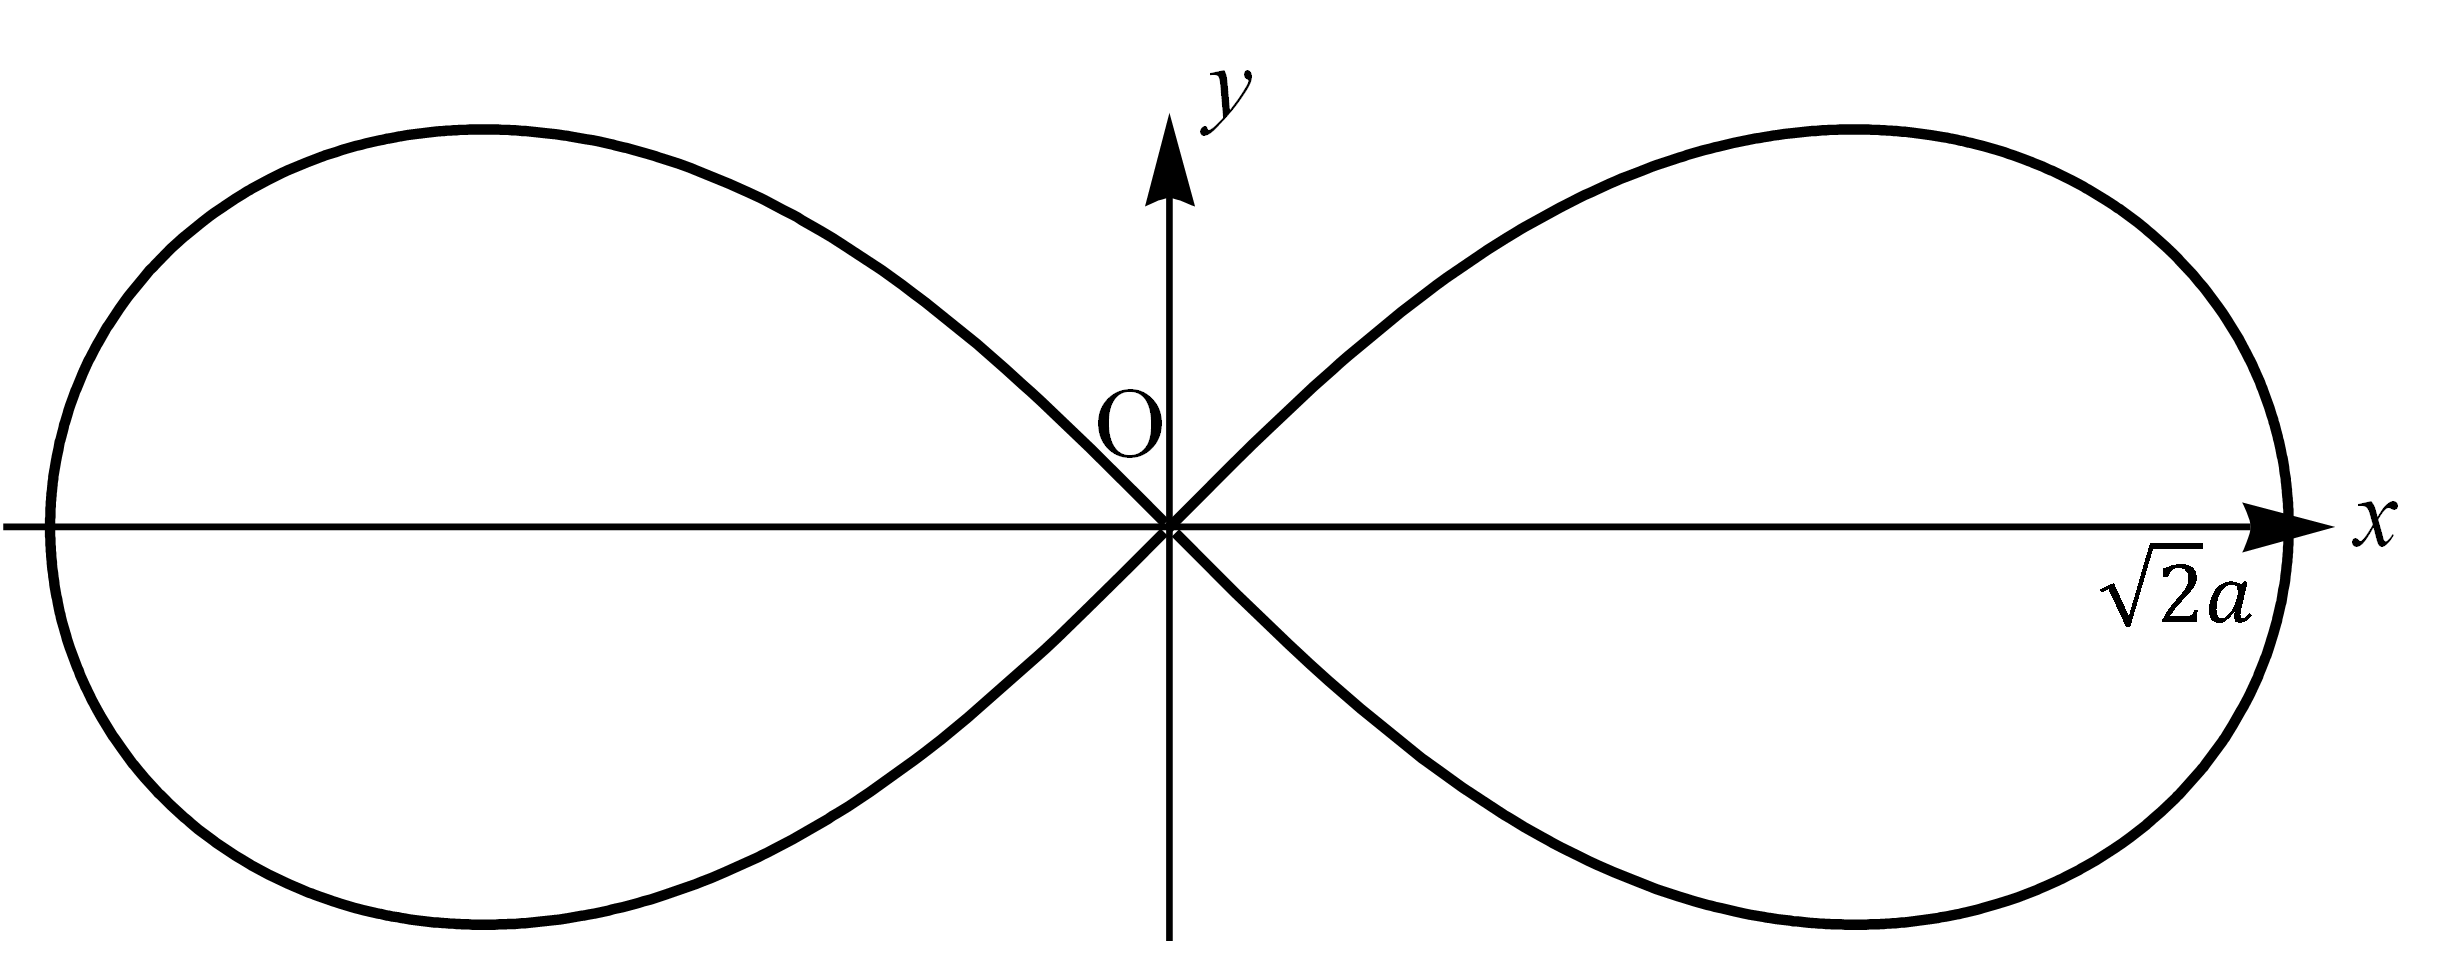
\includegraphics[height=0.2\textwidth]{F:/life/2018AutumnTA/Exercises/11/Fig5-3-3.png}
\end{center}
\caption{习题7.5 3.(3)题图示}
\label{5-3-3}
\end{figure}
将$\rho^2=2a^2\cos2\theta$两边对$\theta$求导得$2\rho\rho'=-4a^2\sin2\theta,\rho'=-\frac{2a^2\sin2\theta}\rho$

$\therefore\rho''=\frac{-4a^2\rho\cos2\theta+2a^2\rho'\sin2\theta}{\rho^2}=\frac{-4a^2\rho\cos2\theta-\frac{2a^2\sin2\theta}\rho2a^2\sin2\theta}{\rho^2}=-\frac{4a^2\rho^2\cos2\theta+4a^4\sin^22\theta}{\rho^3}\\
=-\frac{4a^22a^2\cos2\theta\cos2\theta+4a^4\sin^22\theta}{\rho^3}=-\frac{8a^4\cos^22\theta+4a^4\sin^22\theta}{\rho^3}=-\frac{4a^4\cos^22\theta+4a^4}{\rho^3}$

曲率$k=\frac{|\rho^2+2(\rho')^2-\rho\rho''|}{[\rho^2+(\rho')^2]^{\frac32}}=\frac{|\rho^2+2(-\frac{2a^2\sin2\theta}\rho)^2+\frac{4a^4\cos^22\theta+4a^4}{\rho^3}\rho|}{[\rho^2+(-\frac{2a^2\sin2\theta}\rho)^2]^{\frac32}}=\frac{|\rho^5+8a^4\rho\sin^22\theta+(4a^4\cos^22\theta+4a^4)\rho|}{(\rho^4+4a^4\sin^22\theta)^{\frac32}}\\
=\frac{|\rho^5+8a^4\rho+(-4a^4\cos^22\theta+4a^4)\rho|}{(\rho^4+4a^4-4a^4\cos^22\theta)^{\frac32}}=\frac{|\rho^5+8a^4\rho+(-\rho^4+4a^4)\rho|}{(4a^4)^{\frac32}}=\frac{12a^4\rho}{8a^6}=\frac{3\rho}{2a^2}=\frac{3\sqrt2a\sqrt{\cos2\theta}}{2a^2}=\frac3a\sqrt{\frac{\cos2\theta}2}$.

曲率半径$R=\frac1k=\frac a3\sqrt{\frac2{\cos2\theta}}$.

\item求曲线$y=\mathrm e^x$上弯曲程度最大的点.

解:$y'=\mathrm e^x,y''=\mathrm e^x$

曲率$k=\frac{|y''|}{[1+(y')^2]^{\frac32}}=\frac{\mathrm e^x}{(1+\mathrm e^{2x})^{\frac32}}$

$k'=\frac{\mathrm e^x(1+\mathrm e^{2x})^{\frac32}-\mathrm e^x\frac32(1+\mathrm e^{2x})^{\frac12}2\mathrm e^{2x}}{(1+\mathrm e^{2x})^3}=\frac{\mathrm e^x(1+\mathrm e^{2x})-3\mathrm e^x\mathrm e^{2x}}{(1+\mathrm e^{2x})^{\frac52}}=\frac{\mathrm e^x-2\mathrm e^{3x}}{(1+\mathrm e^{2x})^{\frac52}}=\frac{\mathrm e^x(1-2\mathrm e^{2x})}{(1+\mathrm e^{2x})^{\frac52}}$

当$x=\ln\frac{\sqrt2}2$时,$k'=0$,当$x<\ln\frac{\sqrt2}2$时,$k'>0$,当$x>\ln\frac{\sqrt2}2$时,$k'<0$

$\therefore k(x)$在区间$(-\infty,+\infty)$上处处可导且$x=\ln\frac{\sqrt2}2$是$k(x)$在$(-\infty,+\infty)$上的唯一驻点,且是极大值点,故是最大值点,即曲线$y=\mathrm e^x$上弯曲程度最大的点为$(\ln\frac{\sqrt2}2,\frac{\sqrt2}2)$.

\item求下列曲面所围空间图形的体积:
\newline
(1)椭球面$\frac{x^2}{a^2}+\frac{y^2}{b^2}+\frac{z^2}{c^2}=1$;
\newline
(2)$x^2+y^2+z^2=R^2$与$x^2+y^2=\frac{R^2}4$.

解:(1)椭球面的图形如图~\ref{5-5-1-1}所示,
\begin{figure}[H]
\begin{center}
    \subfloat[]{\label{5-5-1-1} {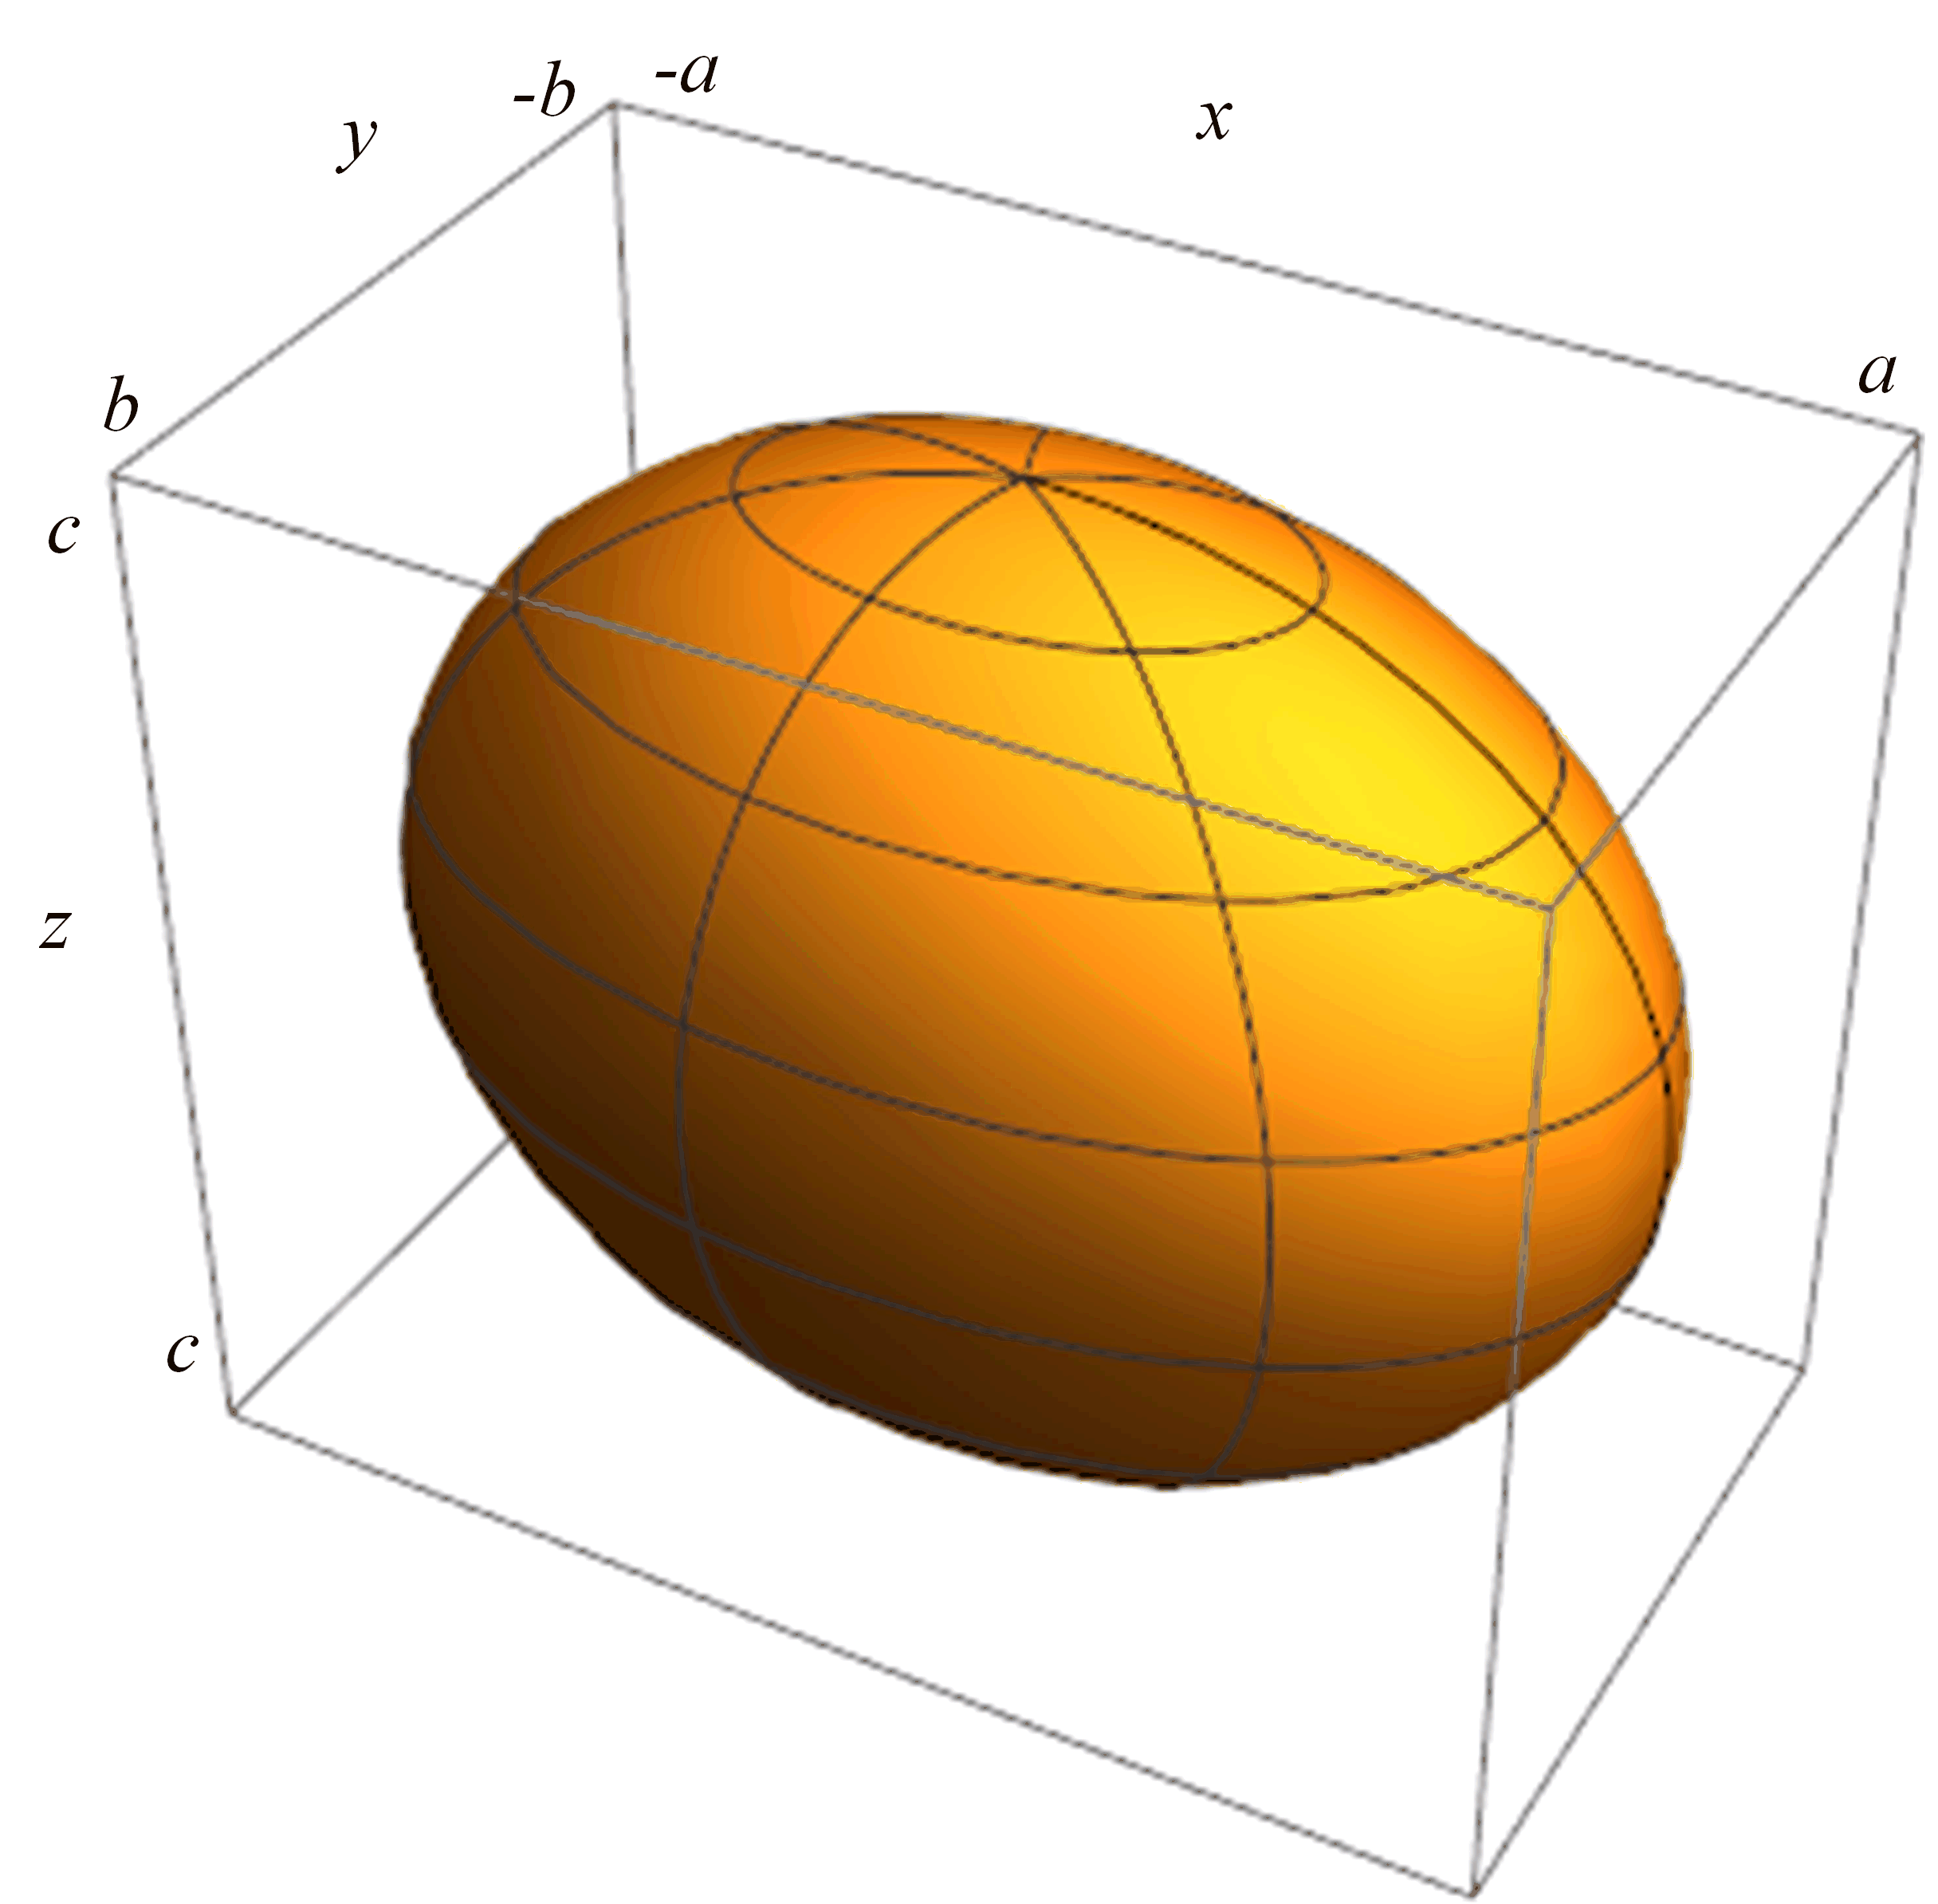
\includegraphics[height=0.3\textheight]{F:/life/2018AutumnTA/Exercises/11/Fig5-5-1-1.png} }}
    \subfloat[]{\label{5-5-1-2} {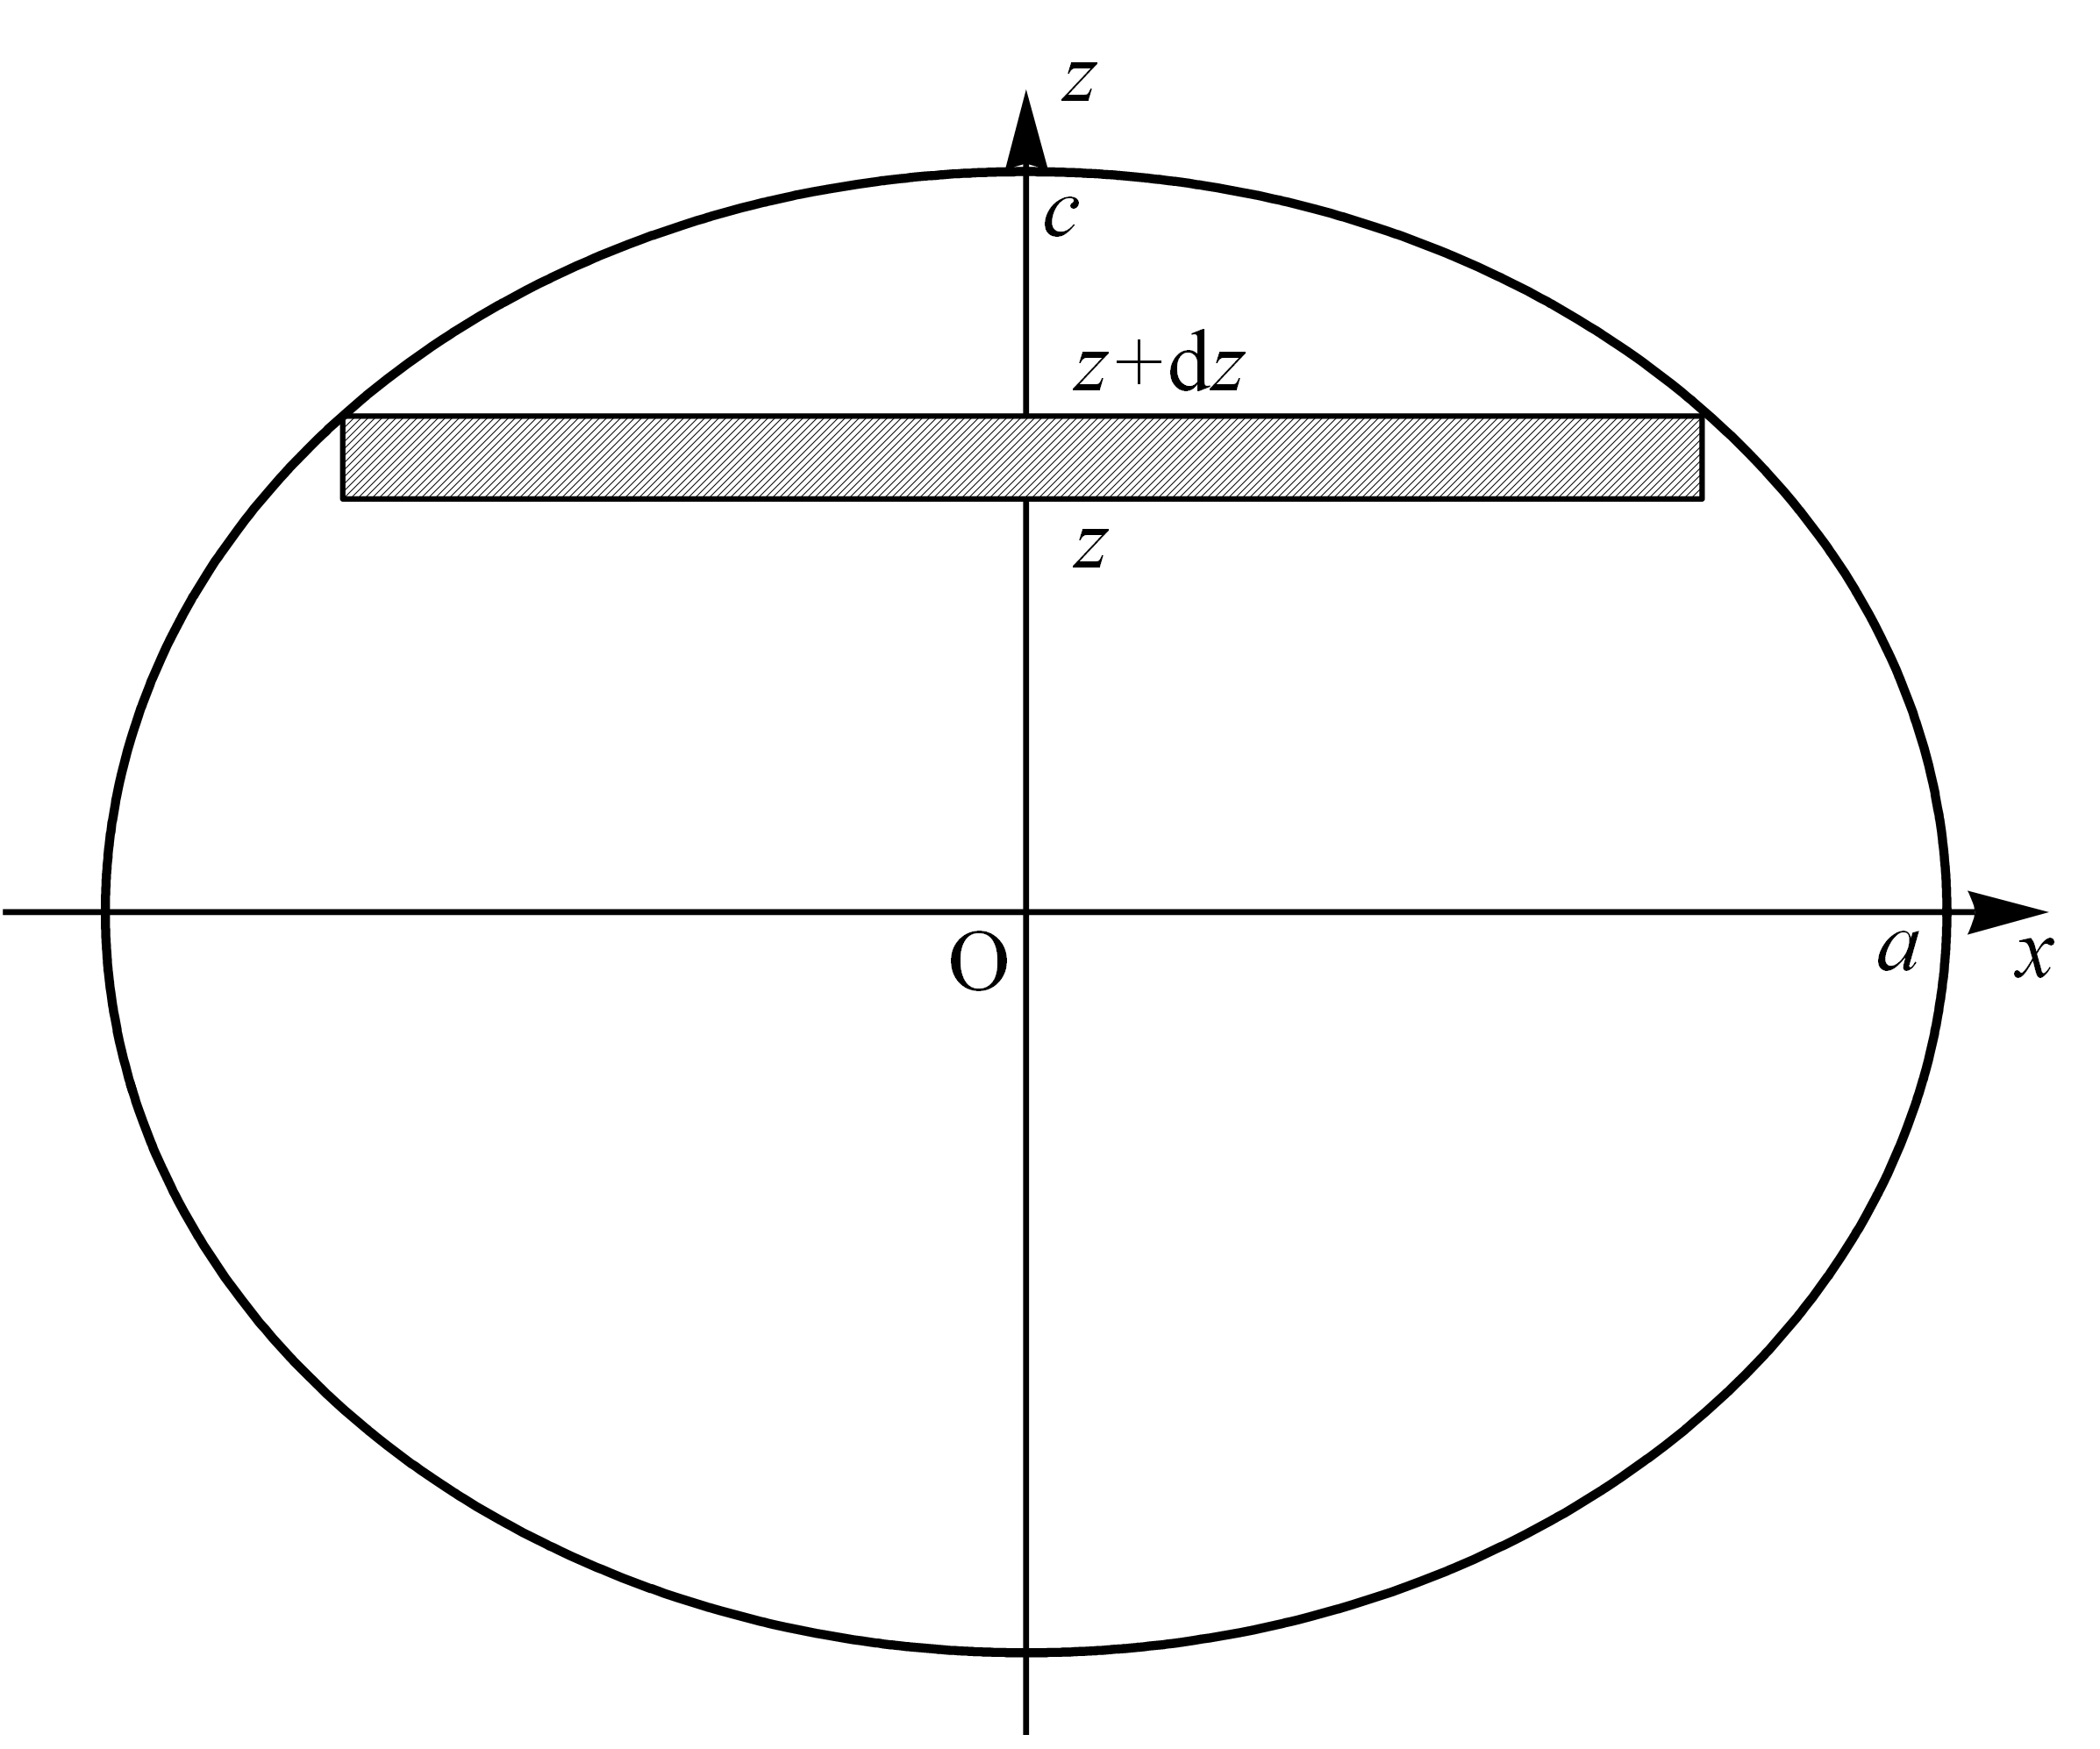
\includegraphics[height=0.3\textheight]{F:/life/2018AutumnTA/Exercises/11/Fig5-5-1-2.png} }}
\end{center}
\caption{习题7.5 5.(1)题图示}
\label{5-5-1}
\end{figure}
竖坐标为$z$时取图~\ref{5-5-1-2}所示的体积元,截面方程为$\frac{x^2}{a^2(1-\frac{z^2}{c^2})}+\frac{y^2}{b^2(1-\frac{z^2}{c^2})}=1$

截面面积$S=\pi a\sqrt{1-\frac{z^2}{c^2}}b\sqrt{1-\frac{z^2}{c^2}}=\pi ab(1-\frac{z^2}{c^2})$

该椭球的体积$V=\int_{-c}^c\pi ab(1-\frac{z^2}{c^2})\mathrm dz=\pi ab(z-\frac1{3c^2}z^3)\Big|_{-c}^c=\frac43\pi abc$.

(2)球面$x^2+y^2+z^2=R^2$和圆柱面$x^2+y^2=\frac{R^2}4$的图形如图~\ref{5-5-2-1}所示,二者所围空间如图~\ref{5-5-2-2}所示,
\begin{figure}[H]
\begin{center}
	\subfloat[]{\label{5-5-2-1}
{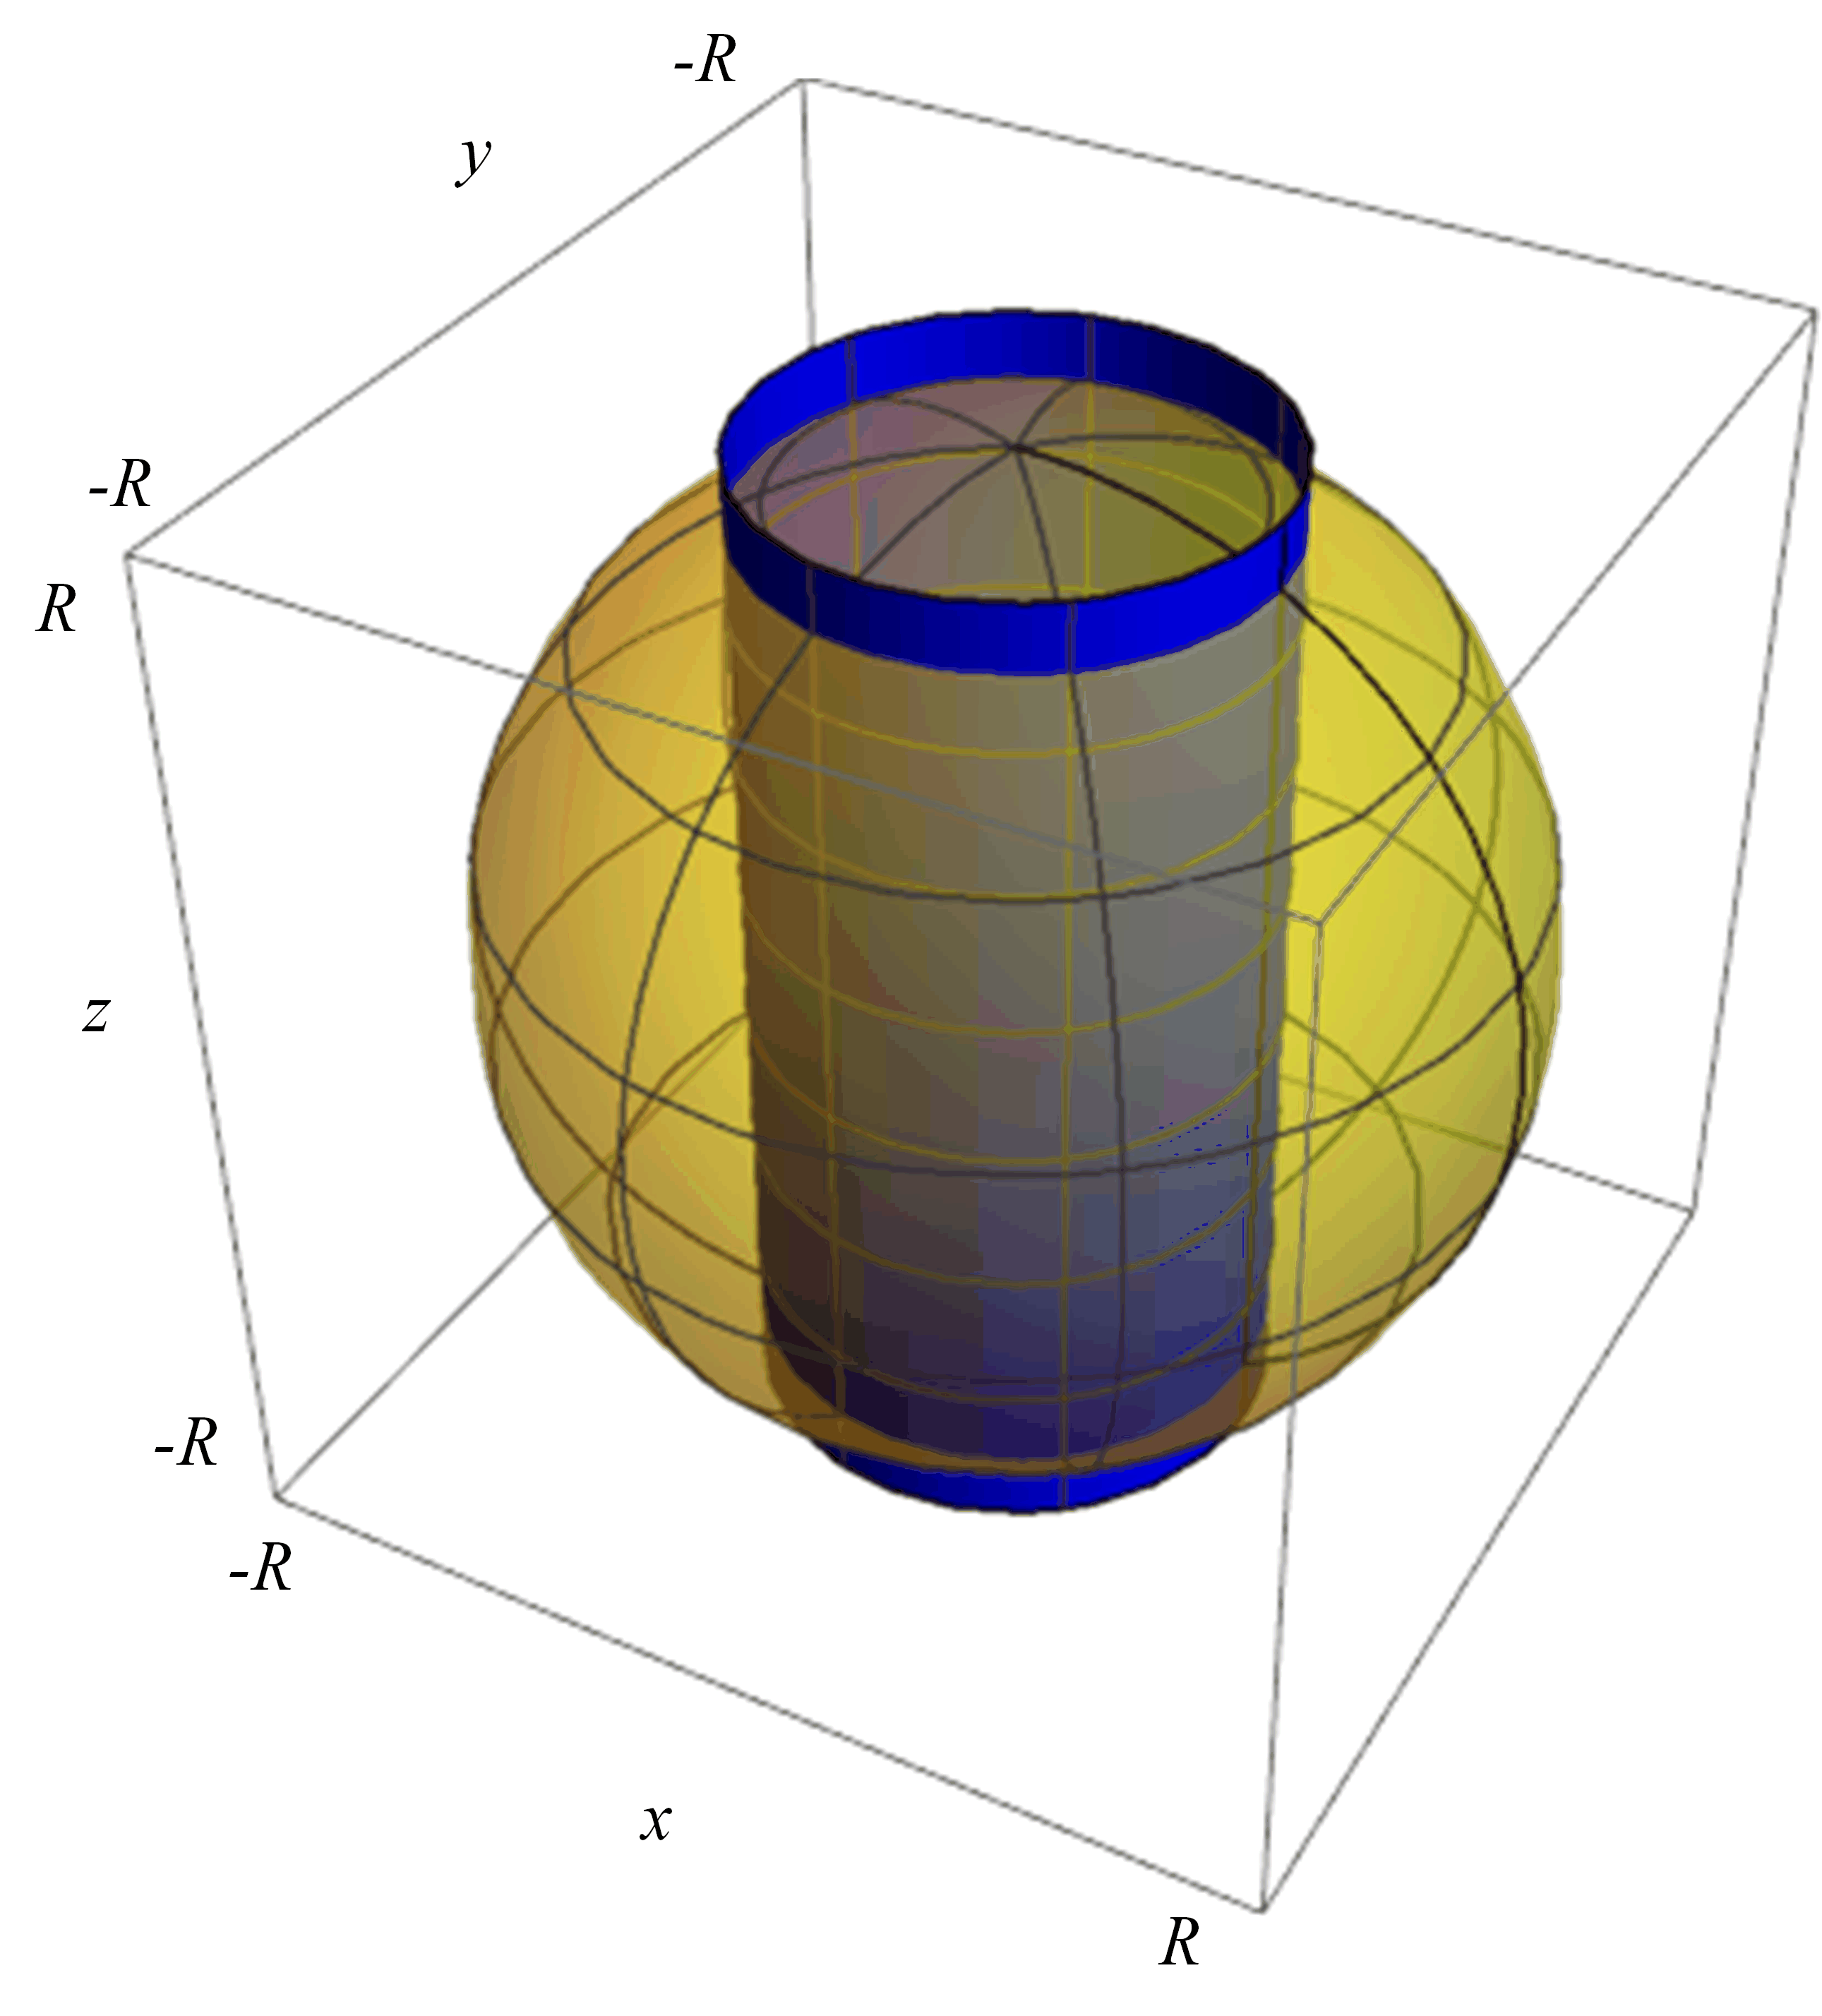
\includegraphics[height=0.4\textheight]{F:/life/2018AutumnTA/Exercises/11/Fig5-5-2-1.png} }}
    \subfloat[]{\label{5-5-2-2} {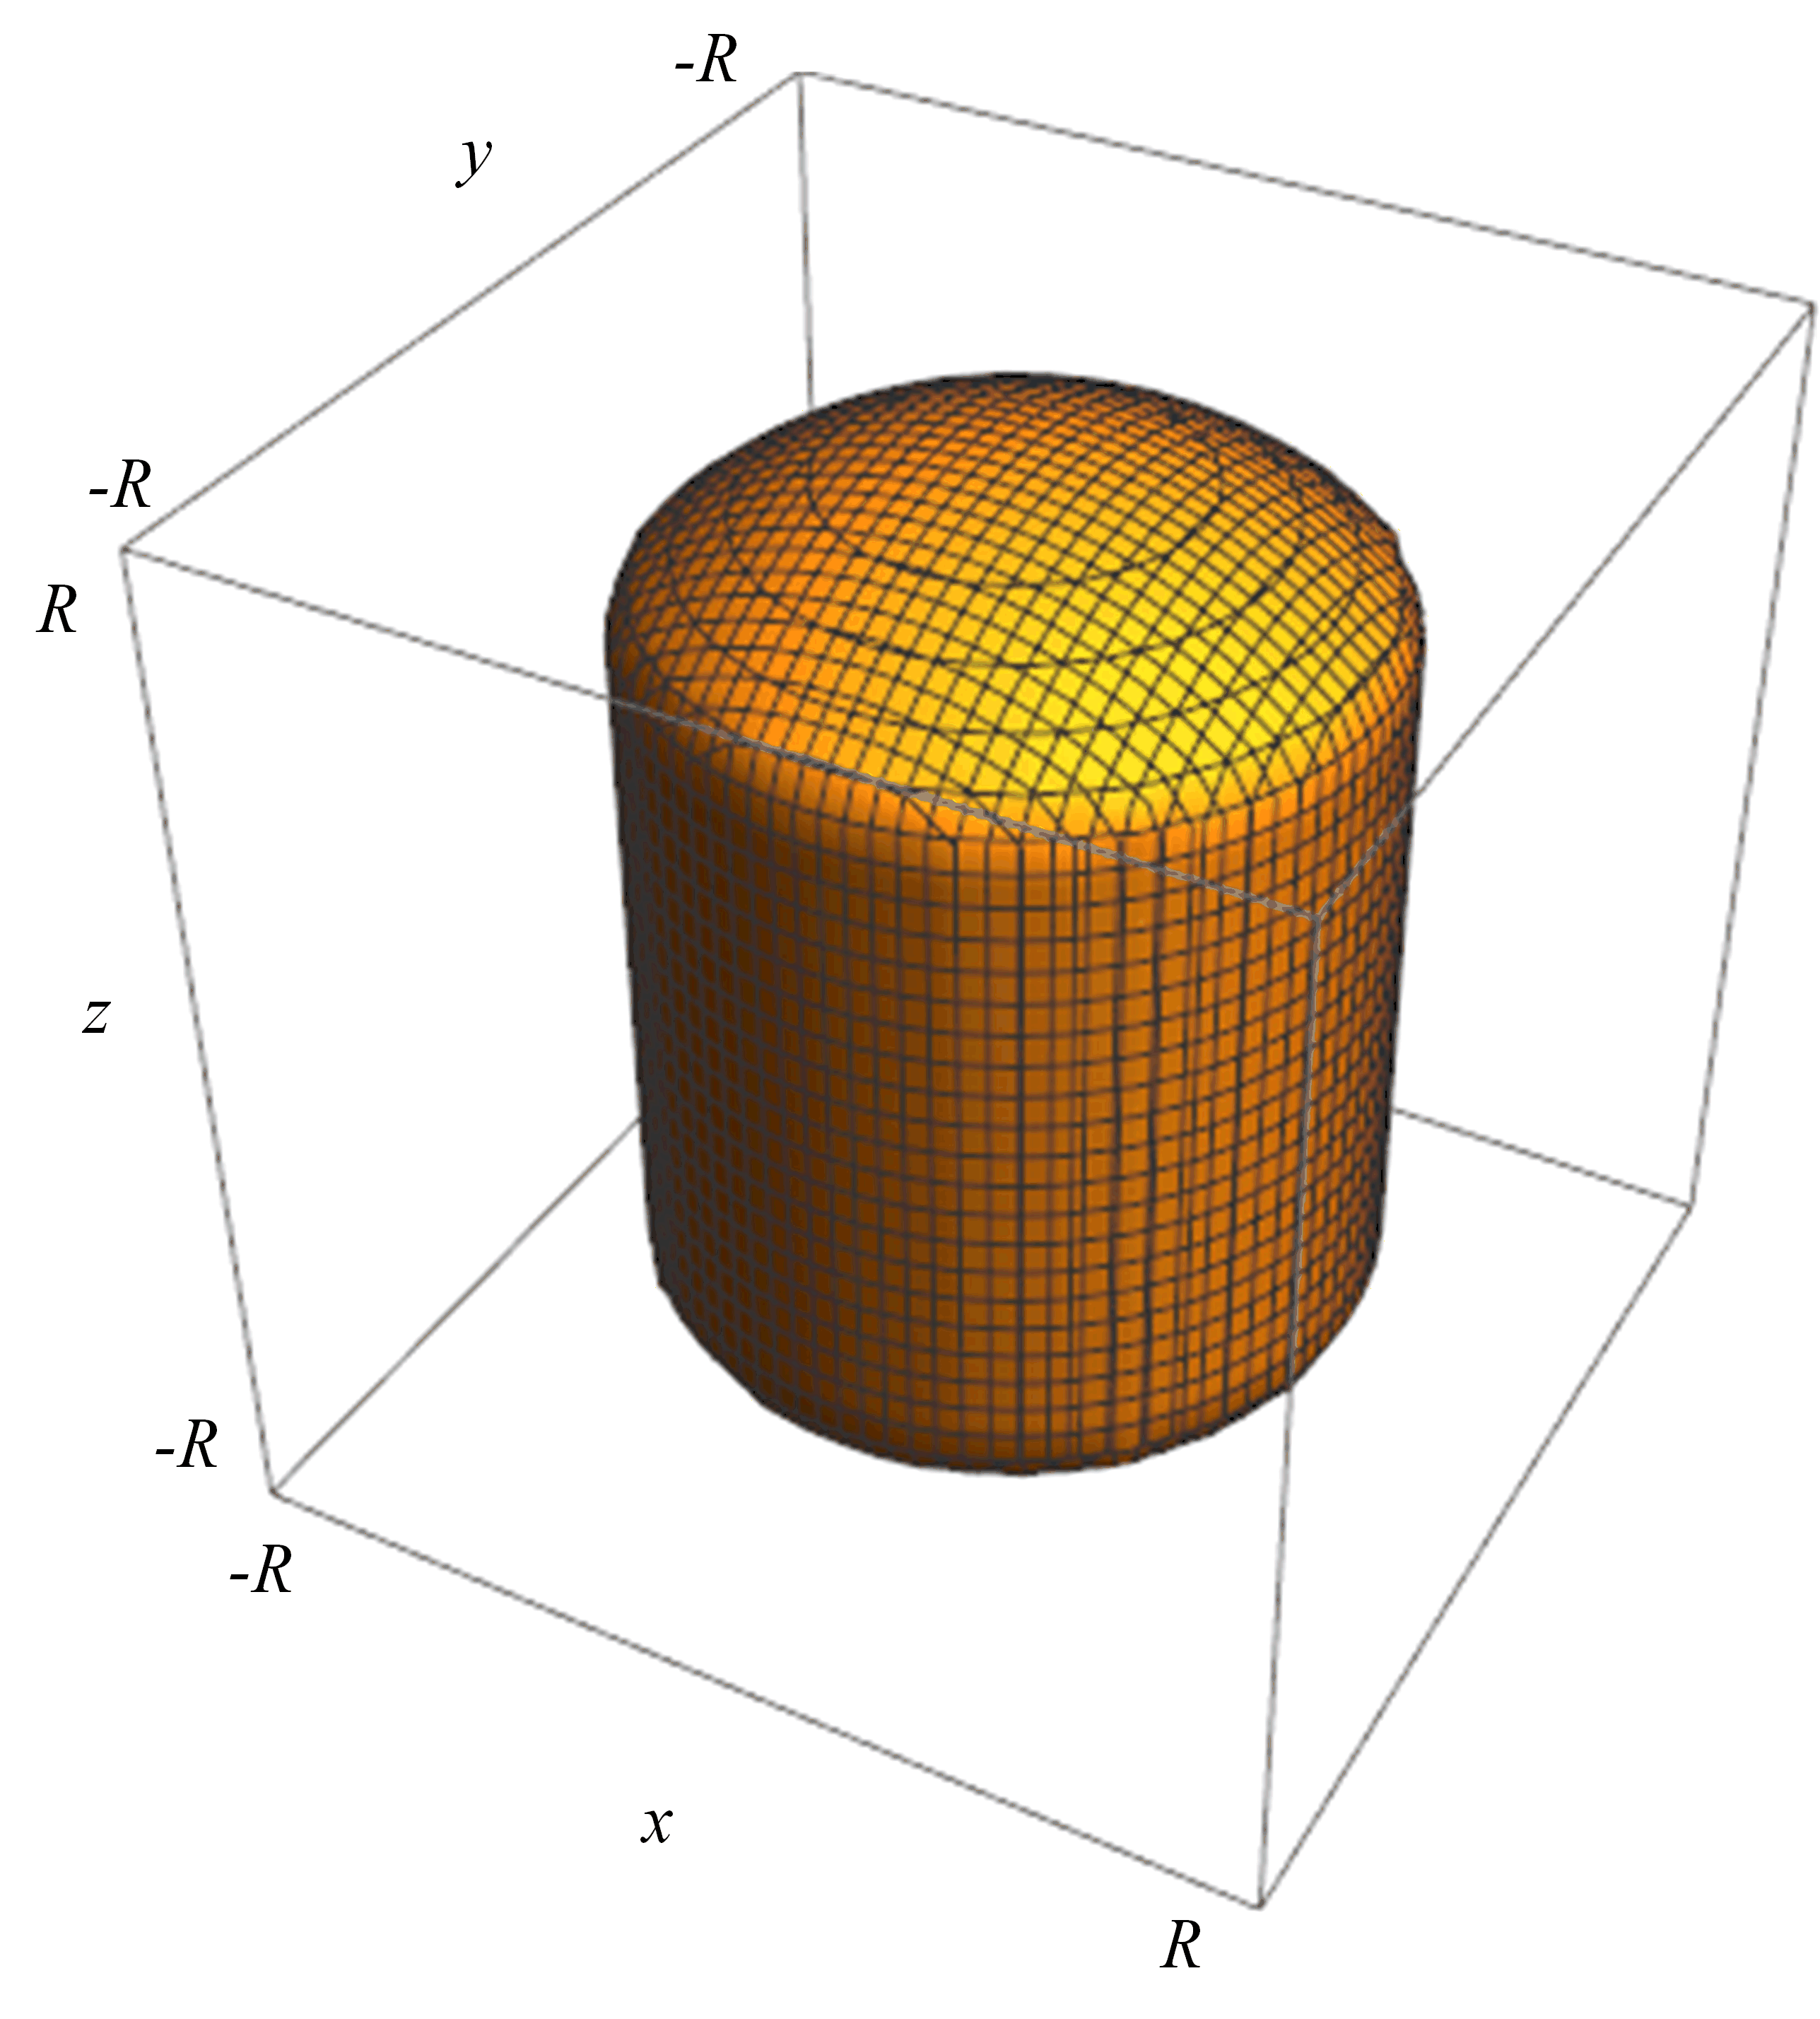
\includegraphics[height=0.4\textheight]{F:/life/2018AutumnTA/Exercises/11/Fig5-5-2-2.png} }}\\
    \subfloat[]{\label{5-5-2-3} {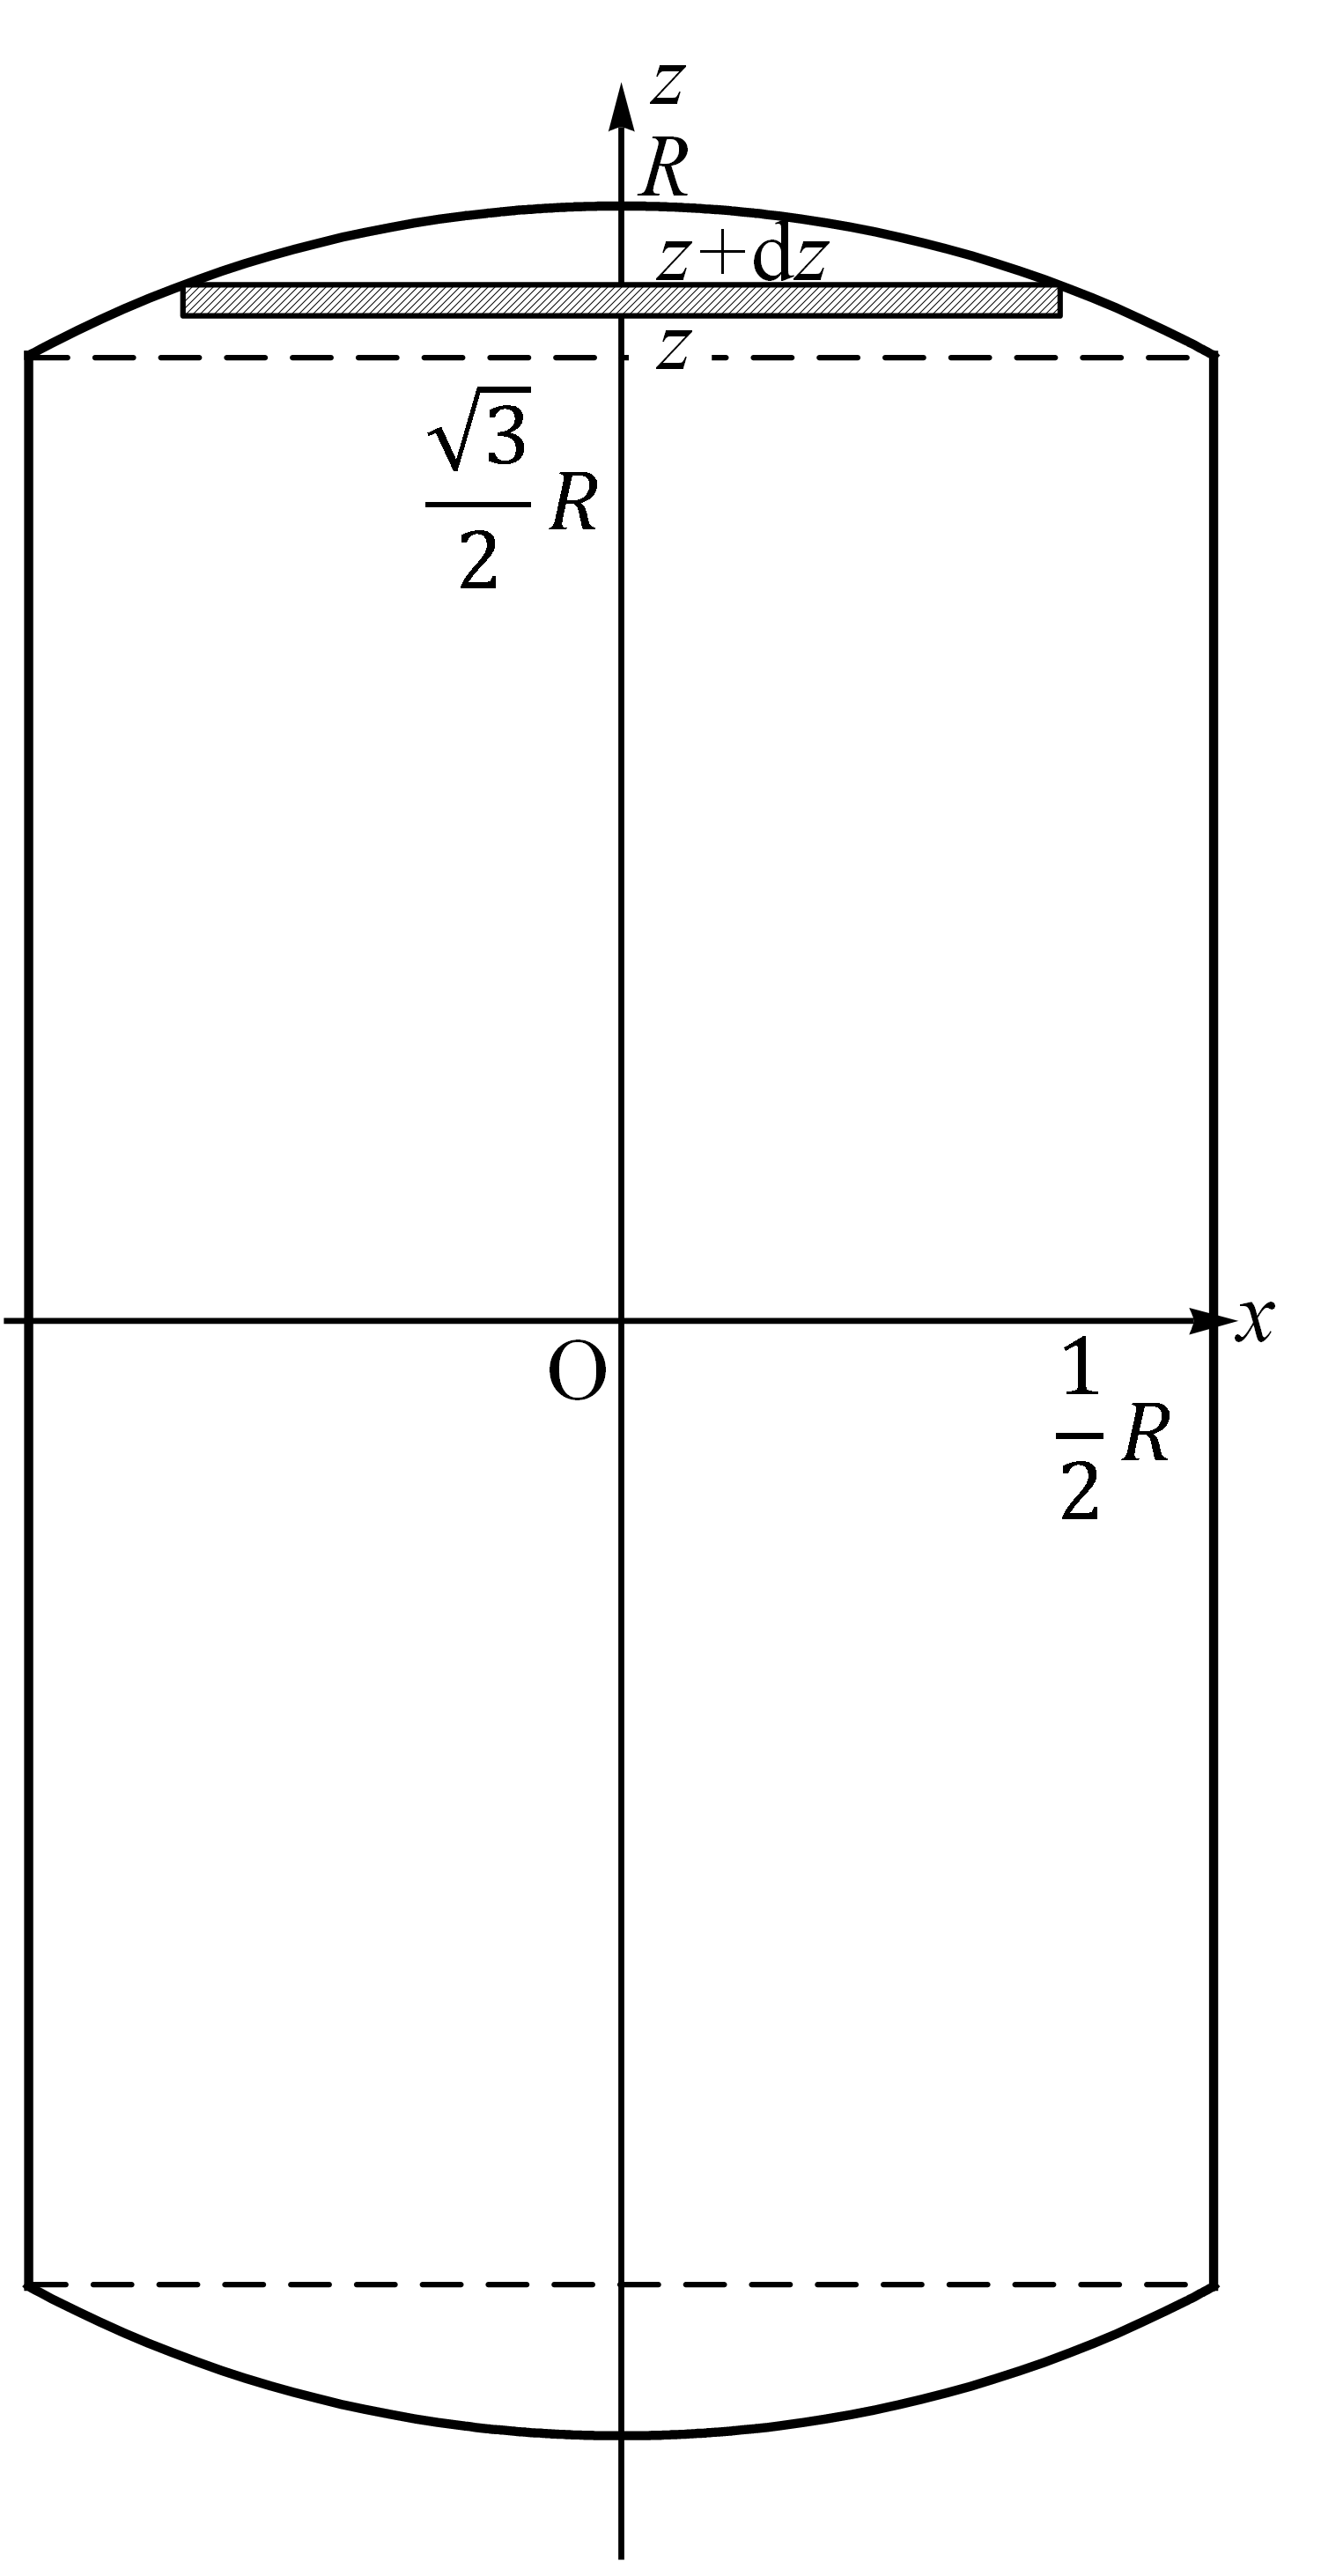
\includegraphics[height=0.4\textheight]{F:/life/2018AutumnTA/Exercises/11/Fig5-5-2-3.png} }}
\end{center}
\caption{习题7.5 5.(2)题图示}
\label{5-5-2}
\end{figure}
由$\begin{cases}
x^2+y^2+z^2=R^2\\
x^2+y^2=\frac{R^2}4
\end{cases}$得$z=\pm\frac{\sqrt3}2R$,故该空间图形可视为高为$\sqrt3R$,半径为$\frac12R$的圆柱和两个半径为$R$,高为$R-\frac{\sqrt3}2R$的球缺组成的组合体

圆柱的体积为$V_1=\pi(\frac12R)^2\cdot\sqrt3R=\frac{\sqrt3}4\pi R^3$

对于球缺,当竖坐标为$z$时取图~\ref{5-5-2-3}所示的体积元,球缺的体积为$V_2=2\int_{\frac{\sqrt3}2R}^R\pi(R^2-z^2)\mathrm dz=2\pi (R^2z-\frac13z^3)\Big|_{\frac{\sqrt3}2R}^R=\frac43\pi R^3-\frac{3\sqrt3}4\pi R^3$

该组合体的体积为$V=V_1+V_2=(\frac43-\frac{\sqrt3}2)\pi R^3$.
\item求下列旋转体的体积:
\newline
(1)$y=\sin x(0\leq x\leq\pi)$绕$x$轴旋转;
\newline
(2)$\begin{cases}
x=a\cos^3t,\\
y=a\sin^3t,
\end{cases}0\leq t\leq2\pi$绕$y$轴,$a>0$;
\newline
(3)$\rho=a(1+\cos\theta)$绕极轴,$a>0$.

解:(1)旋转体如图~\ref{5-6-1-1}所示,取如图~\ref{5-6-1-2}所示的体积元,
\begin{figure}[H]
\begin{center}
 \subfloat[]{\label{5-6-1-1}
{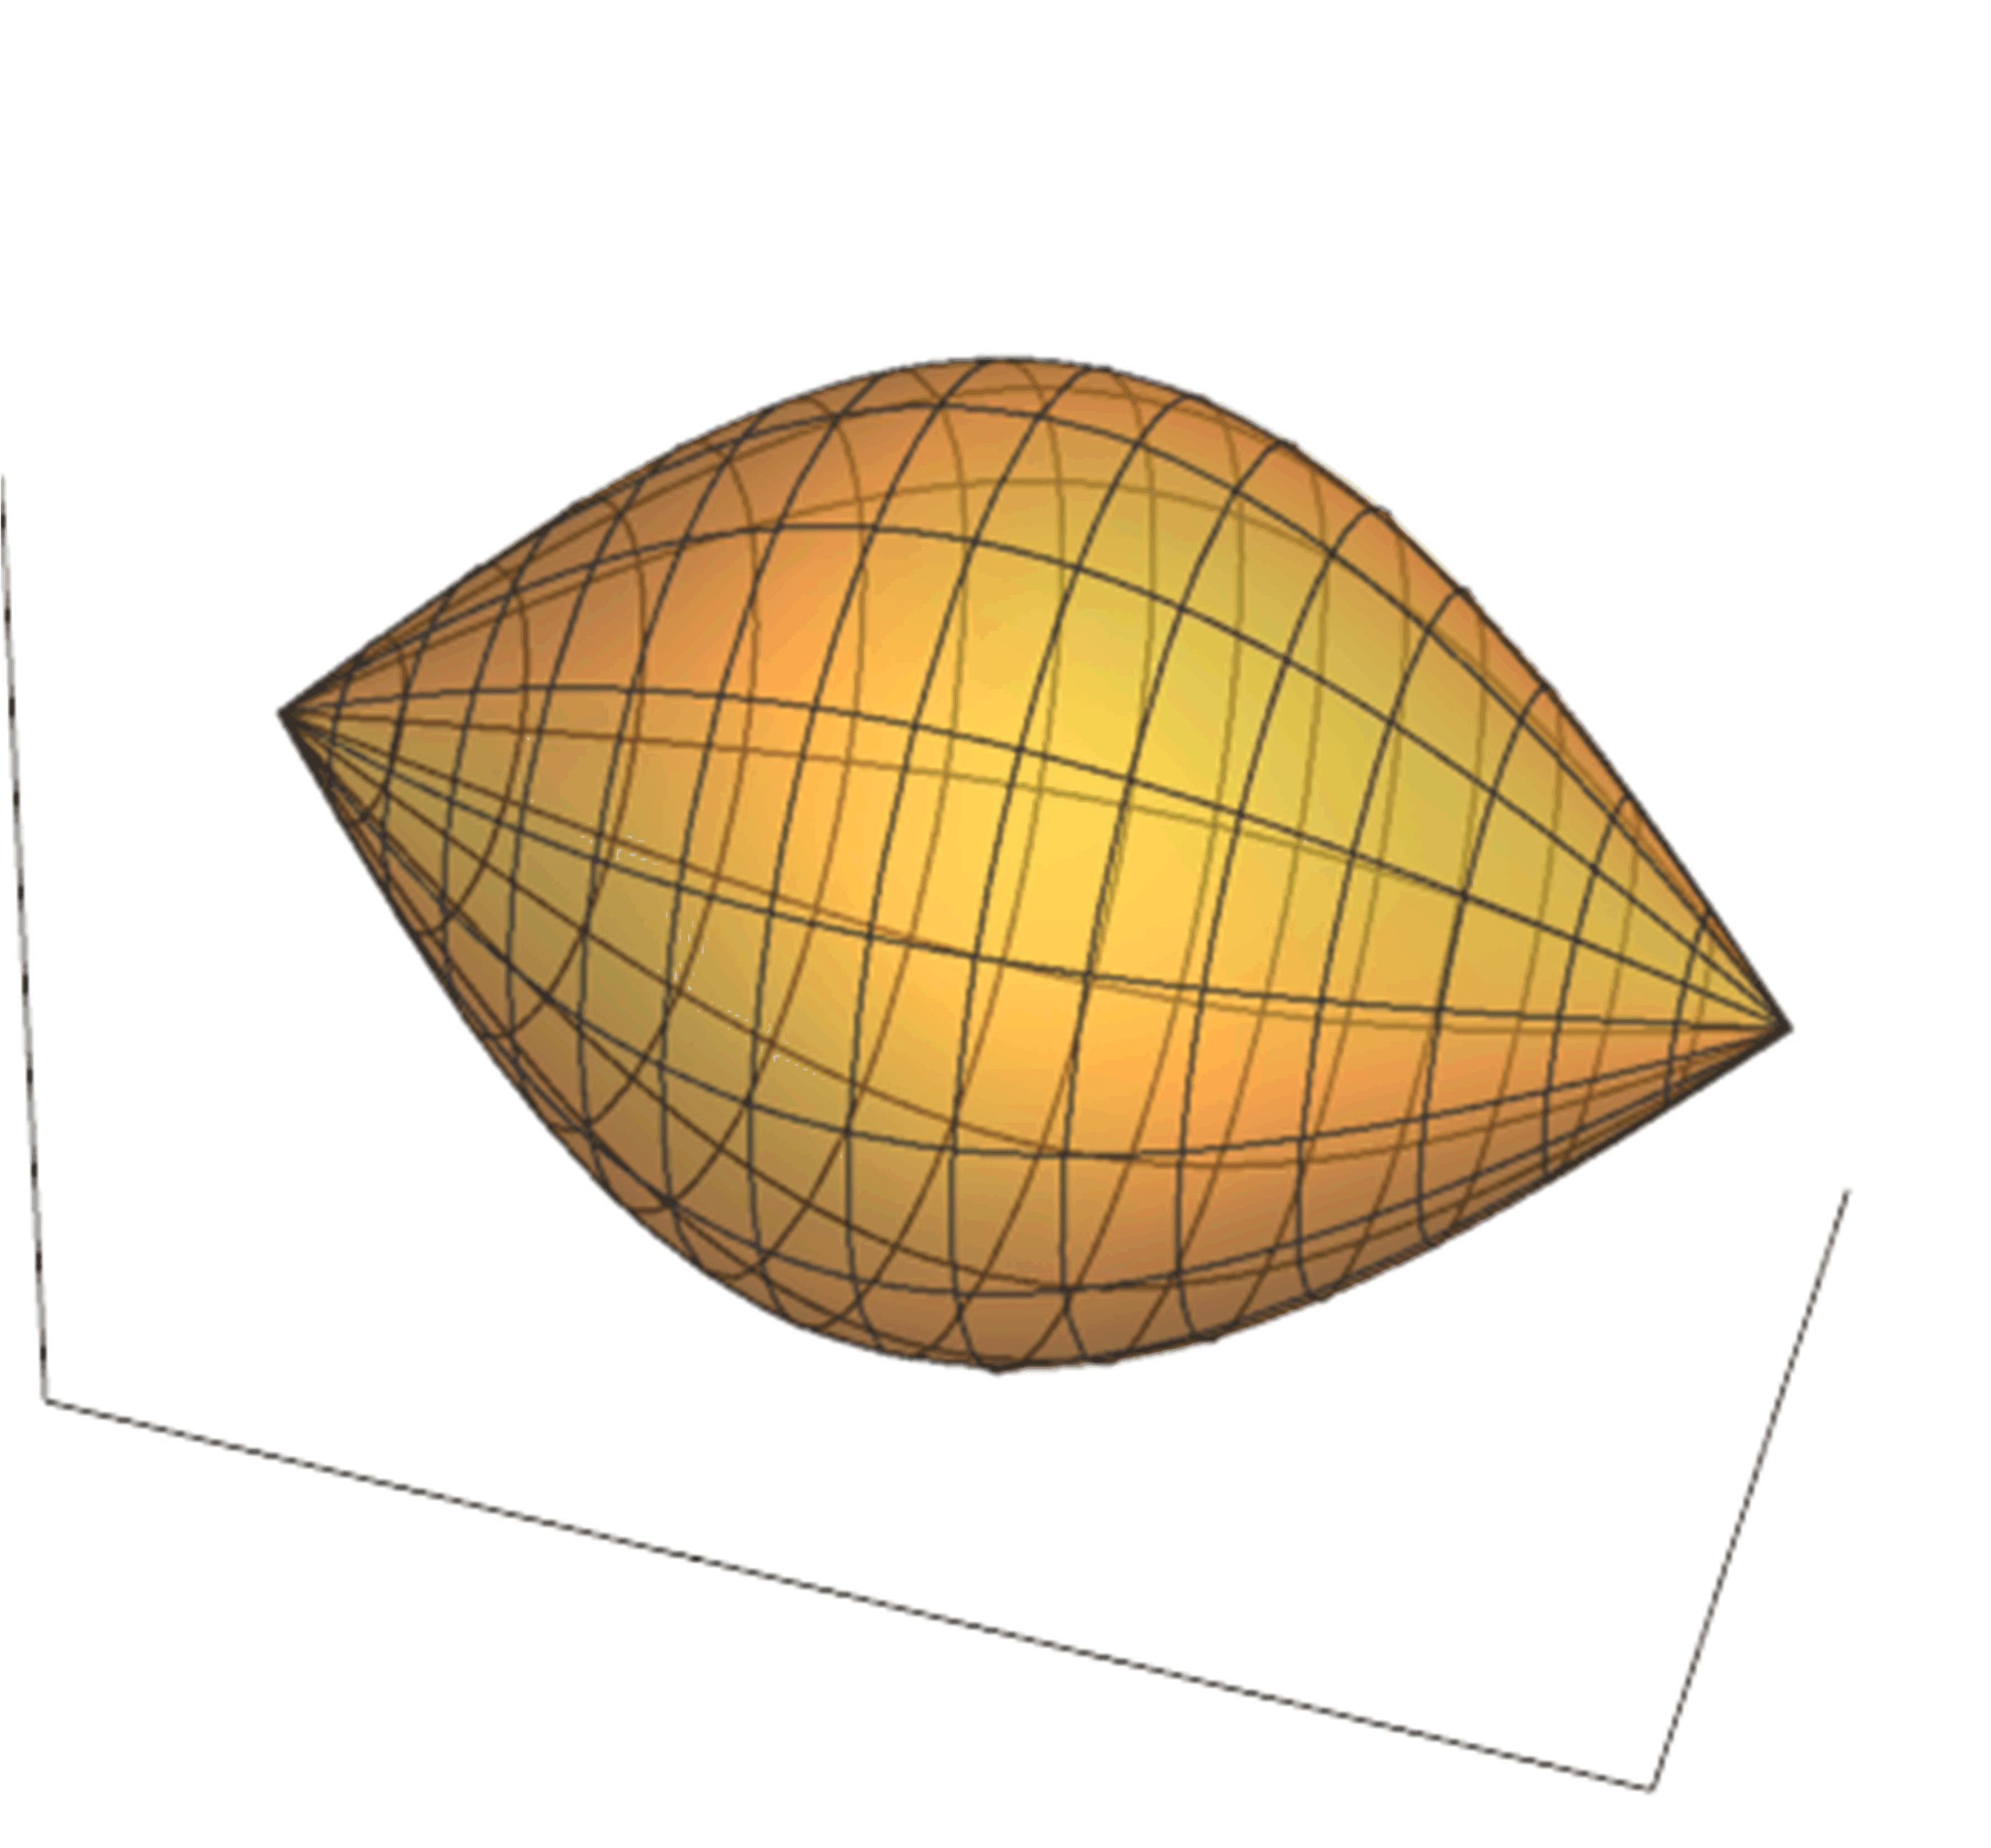
\includegraphics[height=0.3\textheight]{F:/life/2018AutumnTA/Exercises/11/Fig5-6-1-2.png} }}
	\subfloat[]{\label{5-6-1-2}
{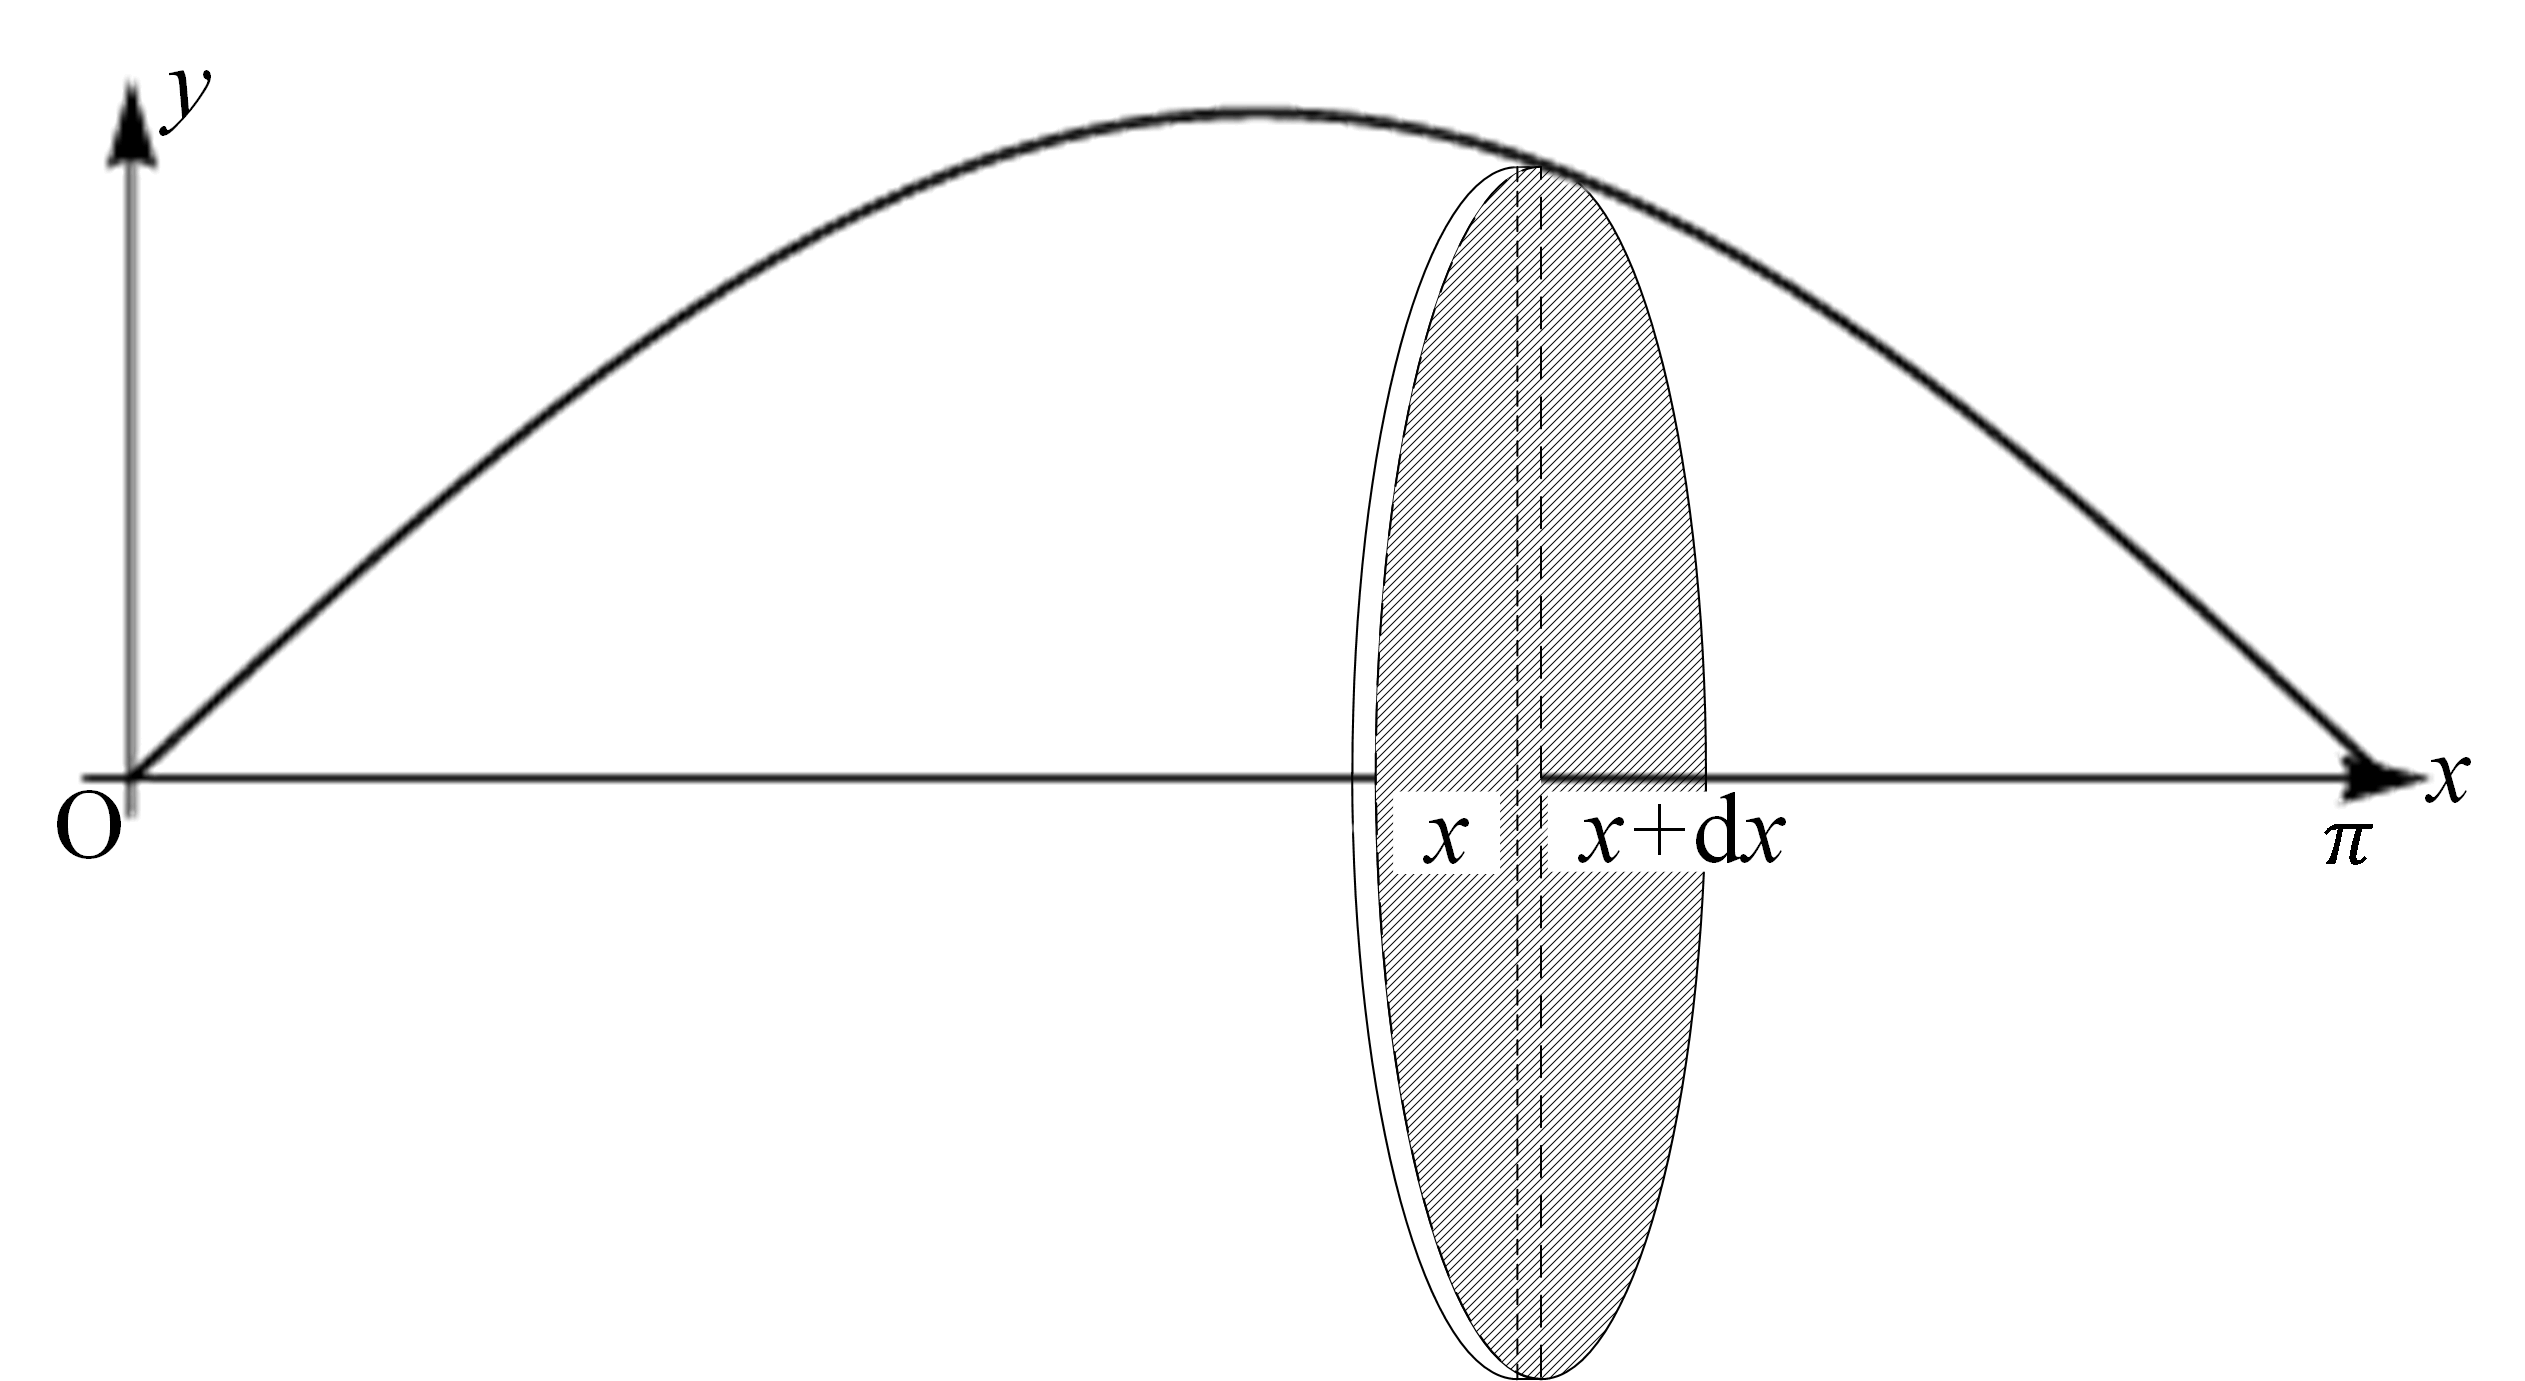
\includegraphics[height=0.2\textheight]{F:/life/2018AutumnTA/Exercises/11/Fig5-6-1-3.png} }}
%    \subfloat[]{\label{5-6-1-2} {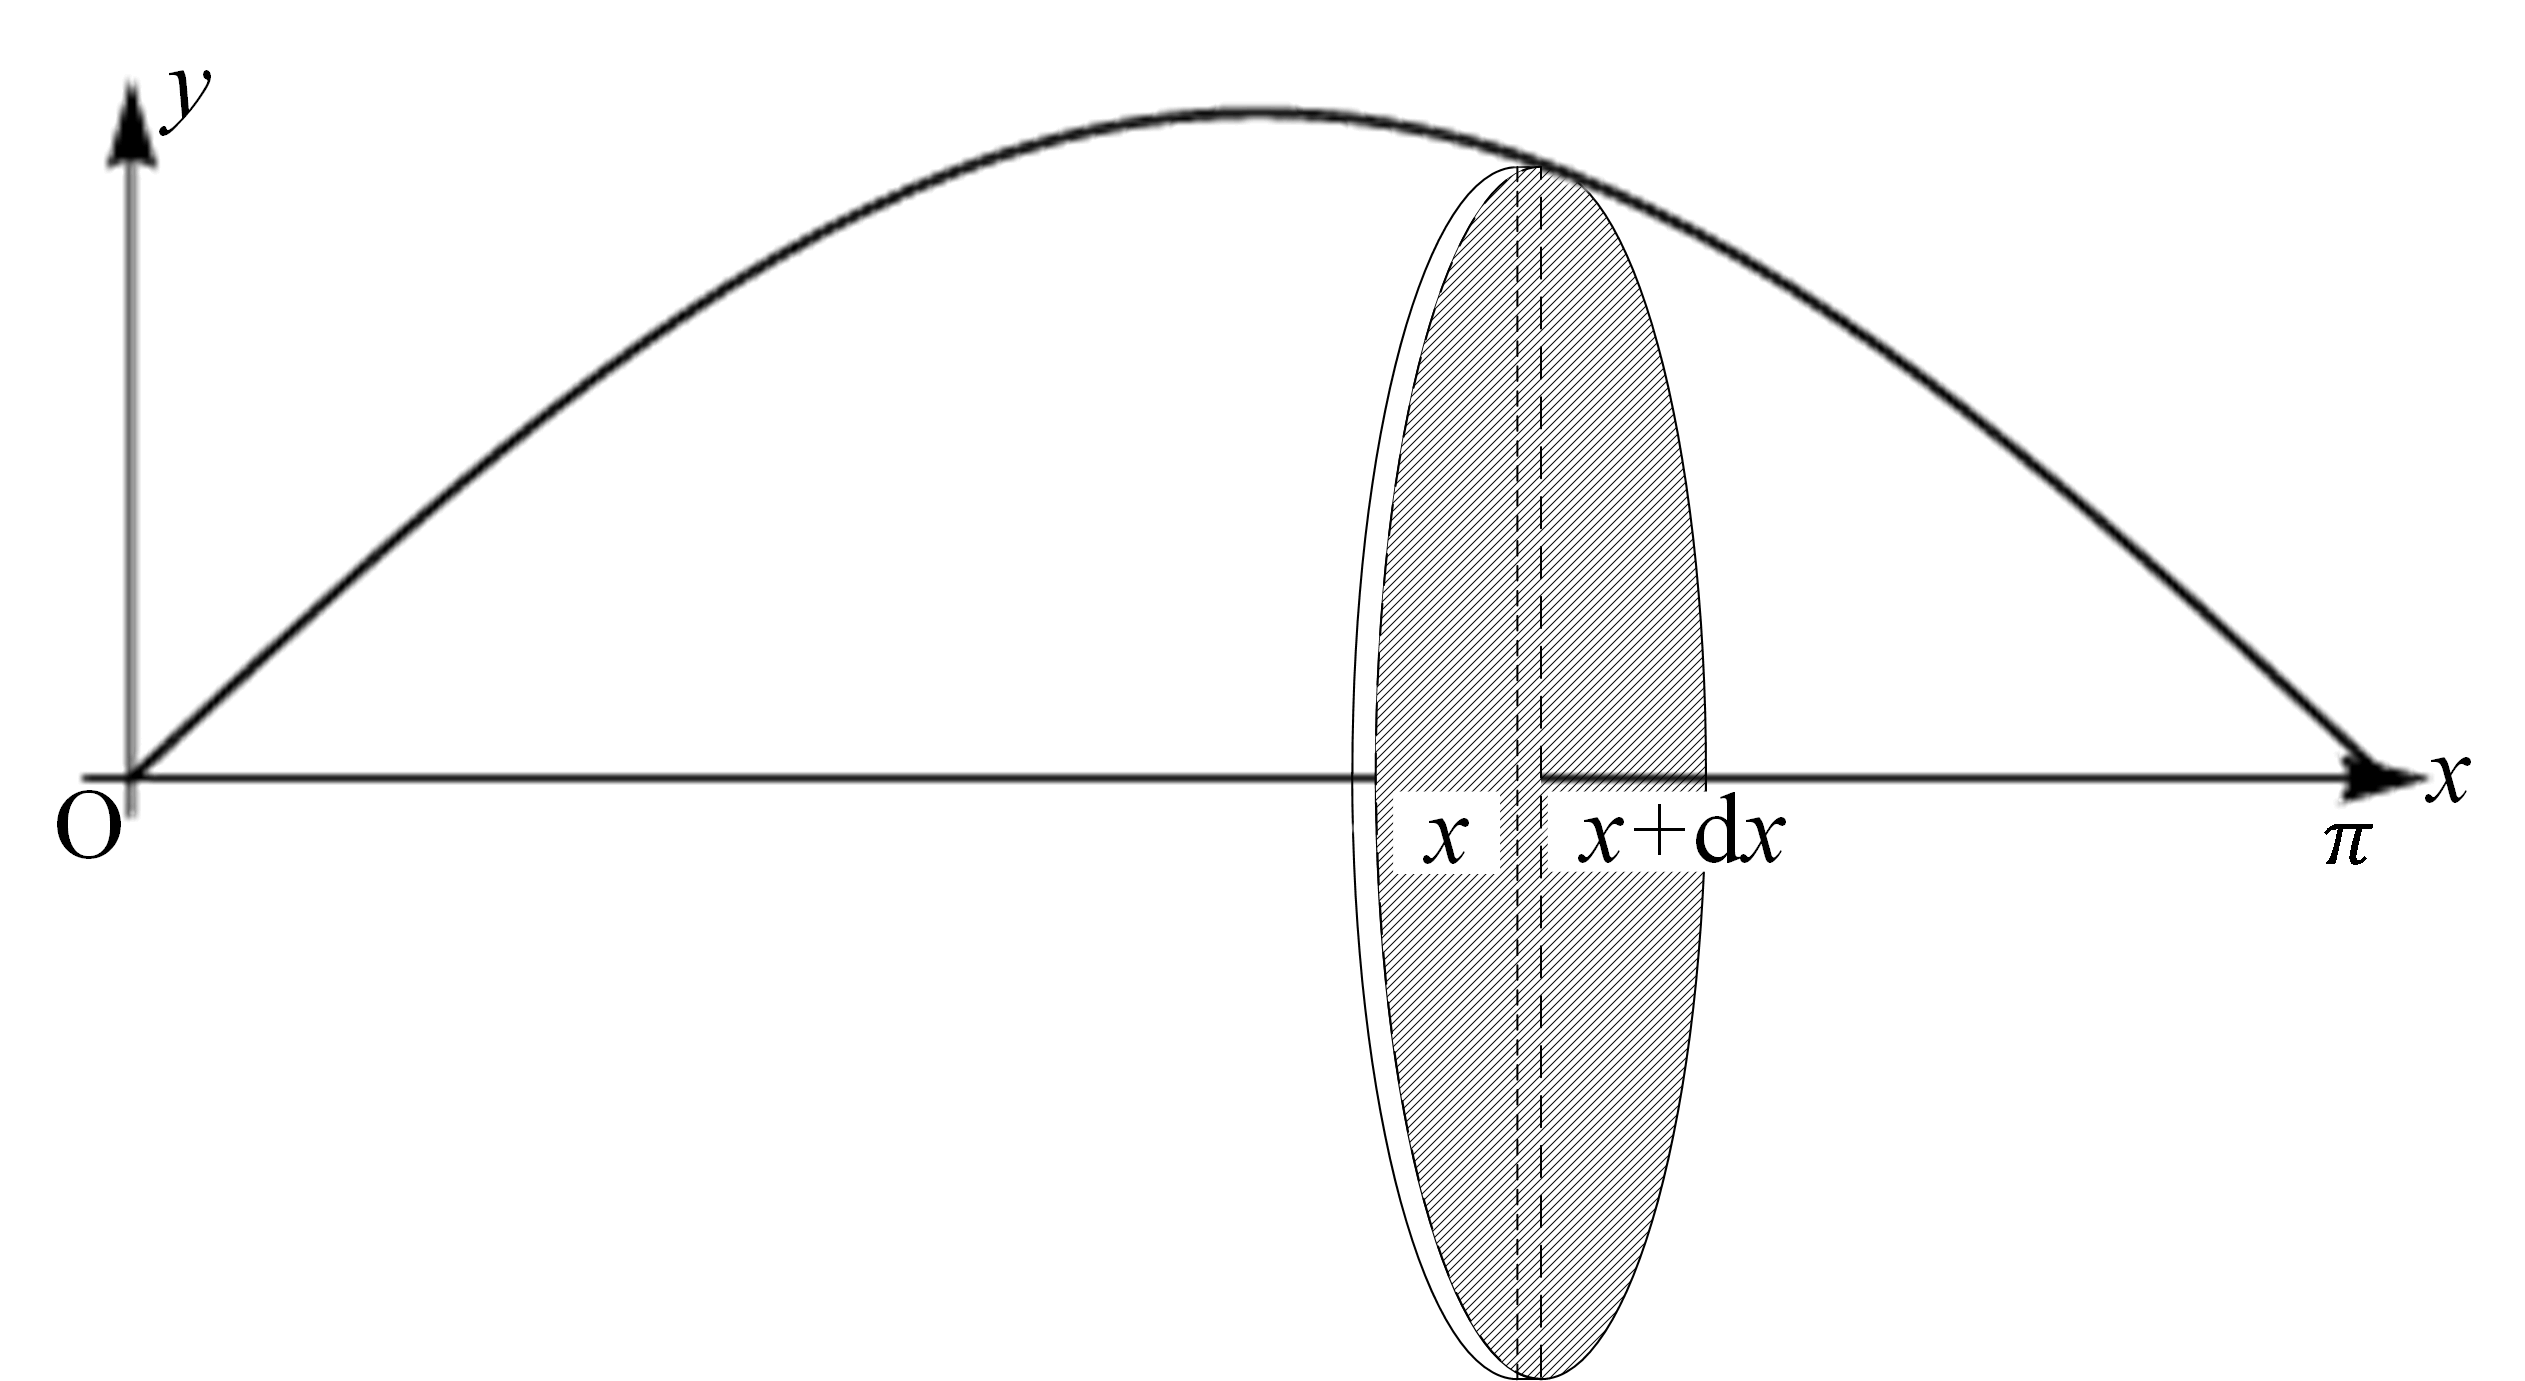
\includegraphics[height=0.2\textheight]{F:/life/2018AutumnTA/Exercises/11/Fig5-6-1-3.png} }}
\end{center}
\caption{习题7.5 6.(1)题图示}
\label{5-6-1}
\end{figure}
旋转体的体积为
\[V=\int_0^\pi\pi y^2\mathrm dx=\int_0^\pi\pi \sin^2x\mathrm dx=2\pi\int_0^{\frac\pi2}\sin^2x\mathrm dx=2\pi\frac12\frac\pi2=\frac{\pi^2}2.\]

(2)$\because x^{\frac23}+y^{\frac23}=a^{\frac23}$

$\therefore$曲线$y=y(x)$关于$x$轴和$y$轴均对称,图形如图~\ref{6-2-a}所示,绕$y$轴旋转得到的旋转体如图~\ref{6-2-b}所示. 
%\begin{figure}[H]
%\begin{center}
%\subfloat[]{\label{6-2-a} {\includegraphics[height=0.3\textheight]{Fig6-2.png} }}
%    \subfloat[]{\label{6-2-b} {\includegraphics[height=0.3\textheight]{Fig6-2-3D.png} }}
%%\begin{tabular}{cc}
%%\includegraphics[height=0.3\textheight]{Fig6-2.png}
%%&\includegraphics[height=0.3\textheight]{Fig6-2-3D.png}
%%\end{tabular}
%\end{center}
%\caption{6.(2)题图示}
%\end{figure}
求该旋转体的体积有以下两种方法:

方法1:对于如图~\ref{6-2-c}所示的切片体积积分,旋转体的体积可以表示为
\[\begin{split}
V&=\int_{-a}^a\pi x^2\mathrm dy=\int_{\frac32\pi}^{\frac12\pi}\pi a^2\cos^6t3a\sin^2t\cos t\mathrm dt=3\pi a^3\int_{\frac32\pi}^{\frac12\pi}(1-\sin^2t)^3\sin^2t\mathrm d\sin t\\
&=3\pi a^3\int_{\frac32\pi}^{\frac12\pi}(1-3\sin^2t+3\sin^4t-\sin^6t)\sin^2t\mathrm d\sin t\\
&=3\pi a^3\int_{\frac32\pi}^{\frac12\pi}(\sin^2t-3\sin^4t+3\sin^6t-\sin^8t)\mathrm d\sin t\\
&=3\pi a^3(\frac13\sin^3t-\frac35\sin^5t+\frac37\sin^7t-\frac19\sin^9t)\Big|_{\frac32\pi}^{\frac12\pi}\\
&=3\pi a^3(\frac13\cdot2-\frac35\cdot2+\frac37\cdot2-\frac19\cdot2)\\
&=\frac{32}{105}\pi a^3.
\end{split}\]

方法2:对于如图~\ref{6-2-d}所示的圆柱壳体积积分,旋转体的体积可以表示为
\[\begin{split}
V&=\int_0^{a}2\pi x\cdot2y\mathrm dx=-\int_{\frac12\pi}^02\pi a\cos^3t\cdot2a\sin^3t\cdot3a\cos^2t\sin t\mathrm dt\\
&=-12\pi a^3\int_{\frac12\pi}^0\sin^4t\cos^4t\mathrm d\sin t\\
&=12\pi a^3\int_0^{\frac12\pi}\sin^4t(1-\sin^2t)^2\mathrm d\sin t\\
&=12\pi a^3\int_0^{\frac12\pi}\sin^4t(1-2\sin^2t+\sin^4t)\mathrm d\sin t\\
&=12\pi a^3\int_0^{\frac12\pi}(\sin^4t-2\sin^6t+\sin^8t)\mathrm d\sin t\\
&=12\pi a^3(\frac15\sin^5t-\frac27\sin^7t+\frac19\sin^9t)\Big|_0^{\frac\pi2}\\
&=12\pi a^3(\frac15-\frac27+\frac19)\\
&=\frac{32}{105}\pi a^3.
\end{split}\]
\begin{figure}[H]
\begin{center}
\subfloat[]{\label{6-2-a}
{\includegraphics[height=0.3\textheight]{F:/life/2018AutumnTA/Exercises/11/Fig6-2.png} }}
    \subfloat[]{\label{6-2-b} {\includegraphics[height=0.3\textheight]{F:/life/2018AutumnTA/Exercises/11/Fig6-2-3D.png} }}\\
    
    \subfloat[]{\label{6-2-c} {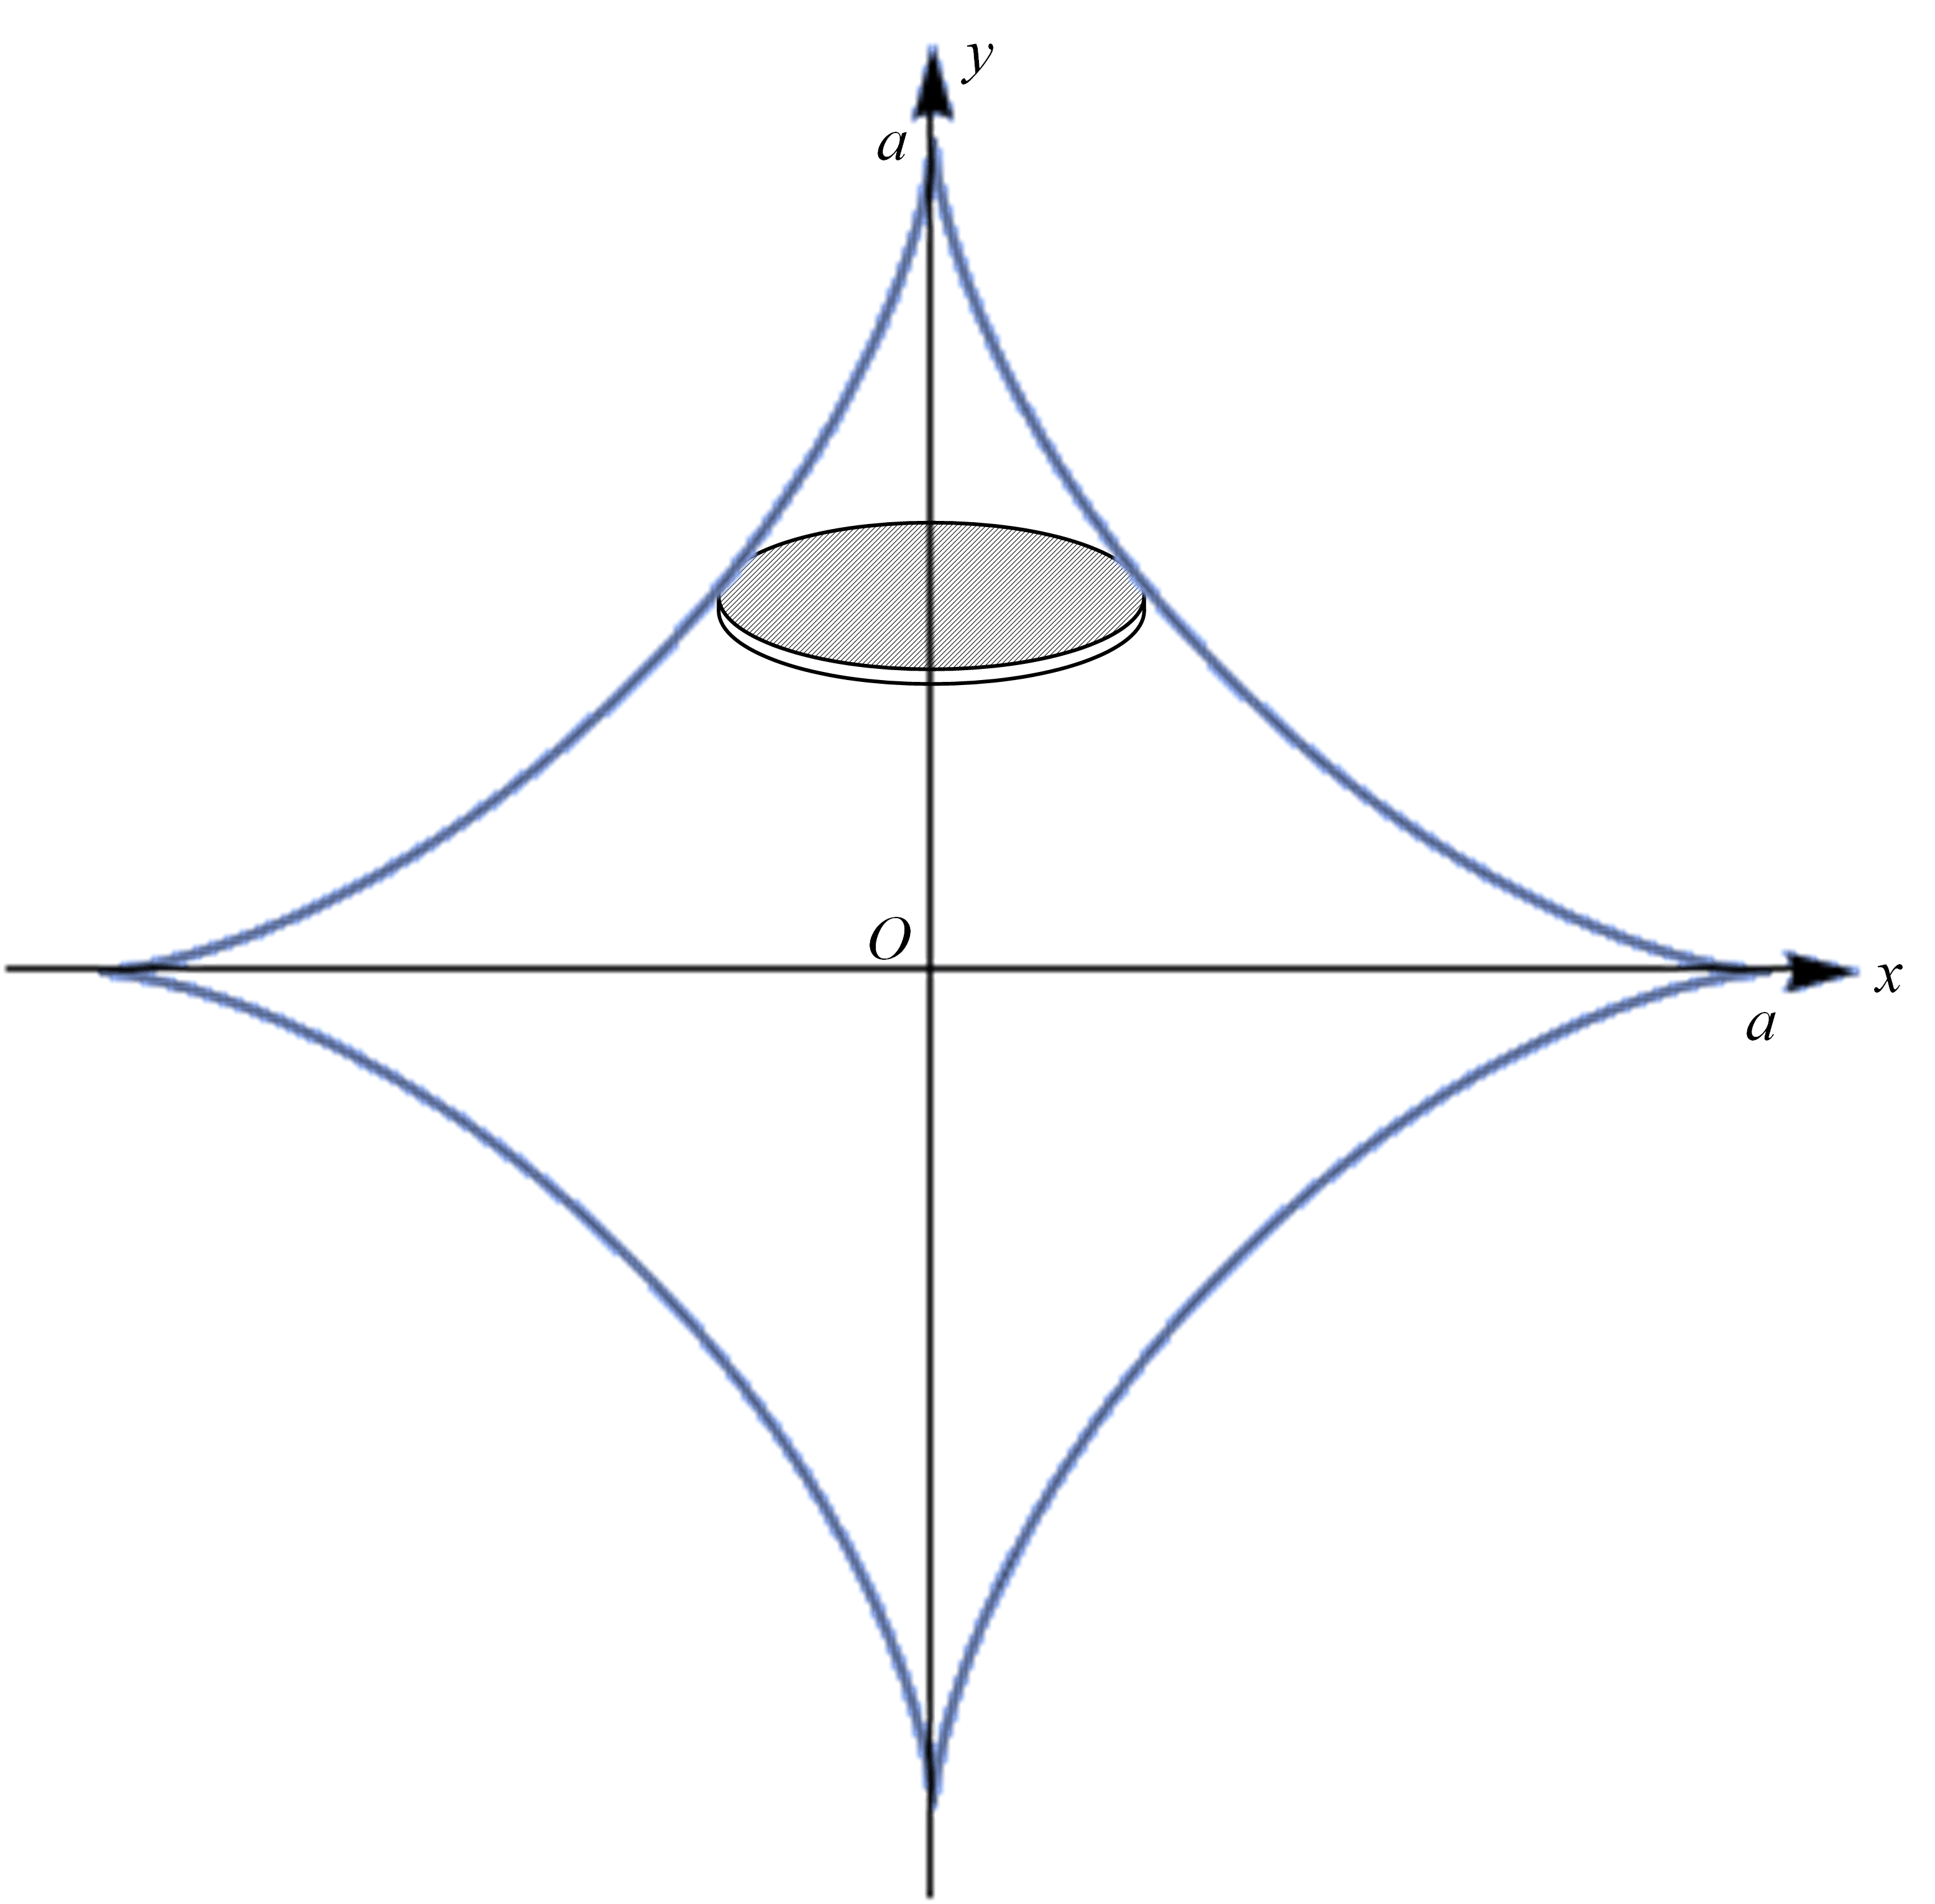
\includegraphics[height=0.3\textheight]{F:/life/2018AutumnTA/Exercises/11/Fig6-2-1.png} }}
    \subfloat[]{\label{6-2-d} {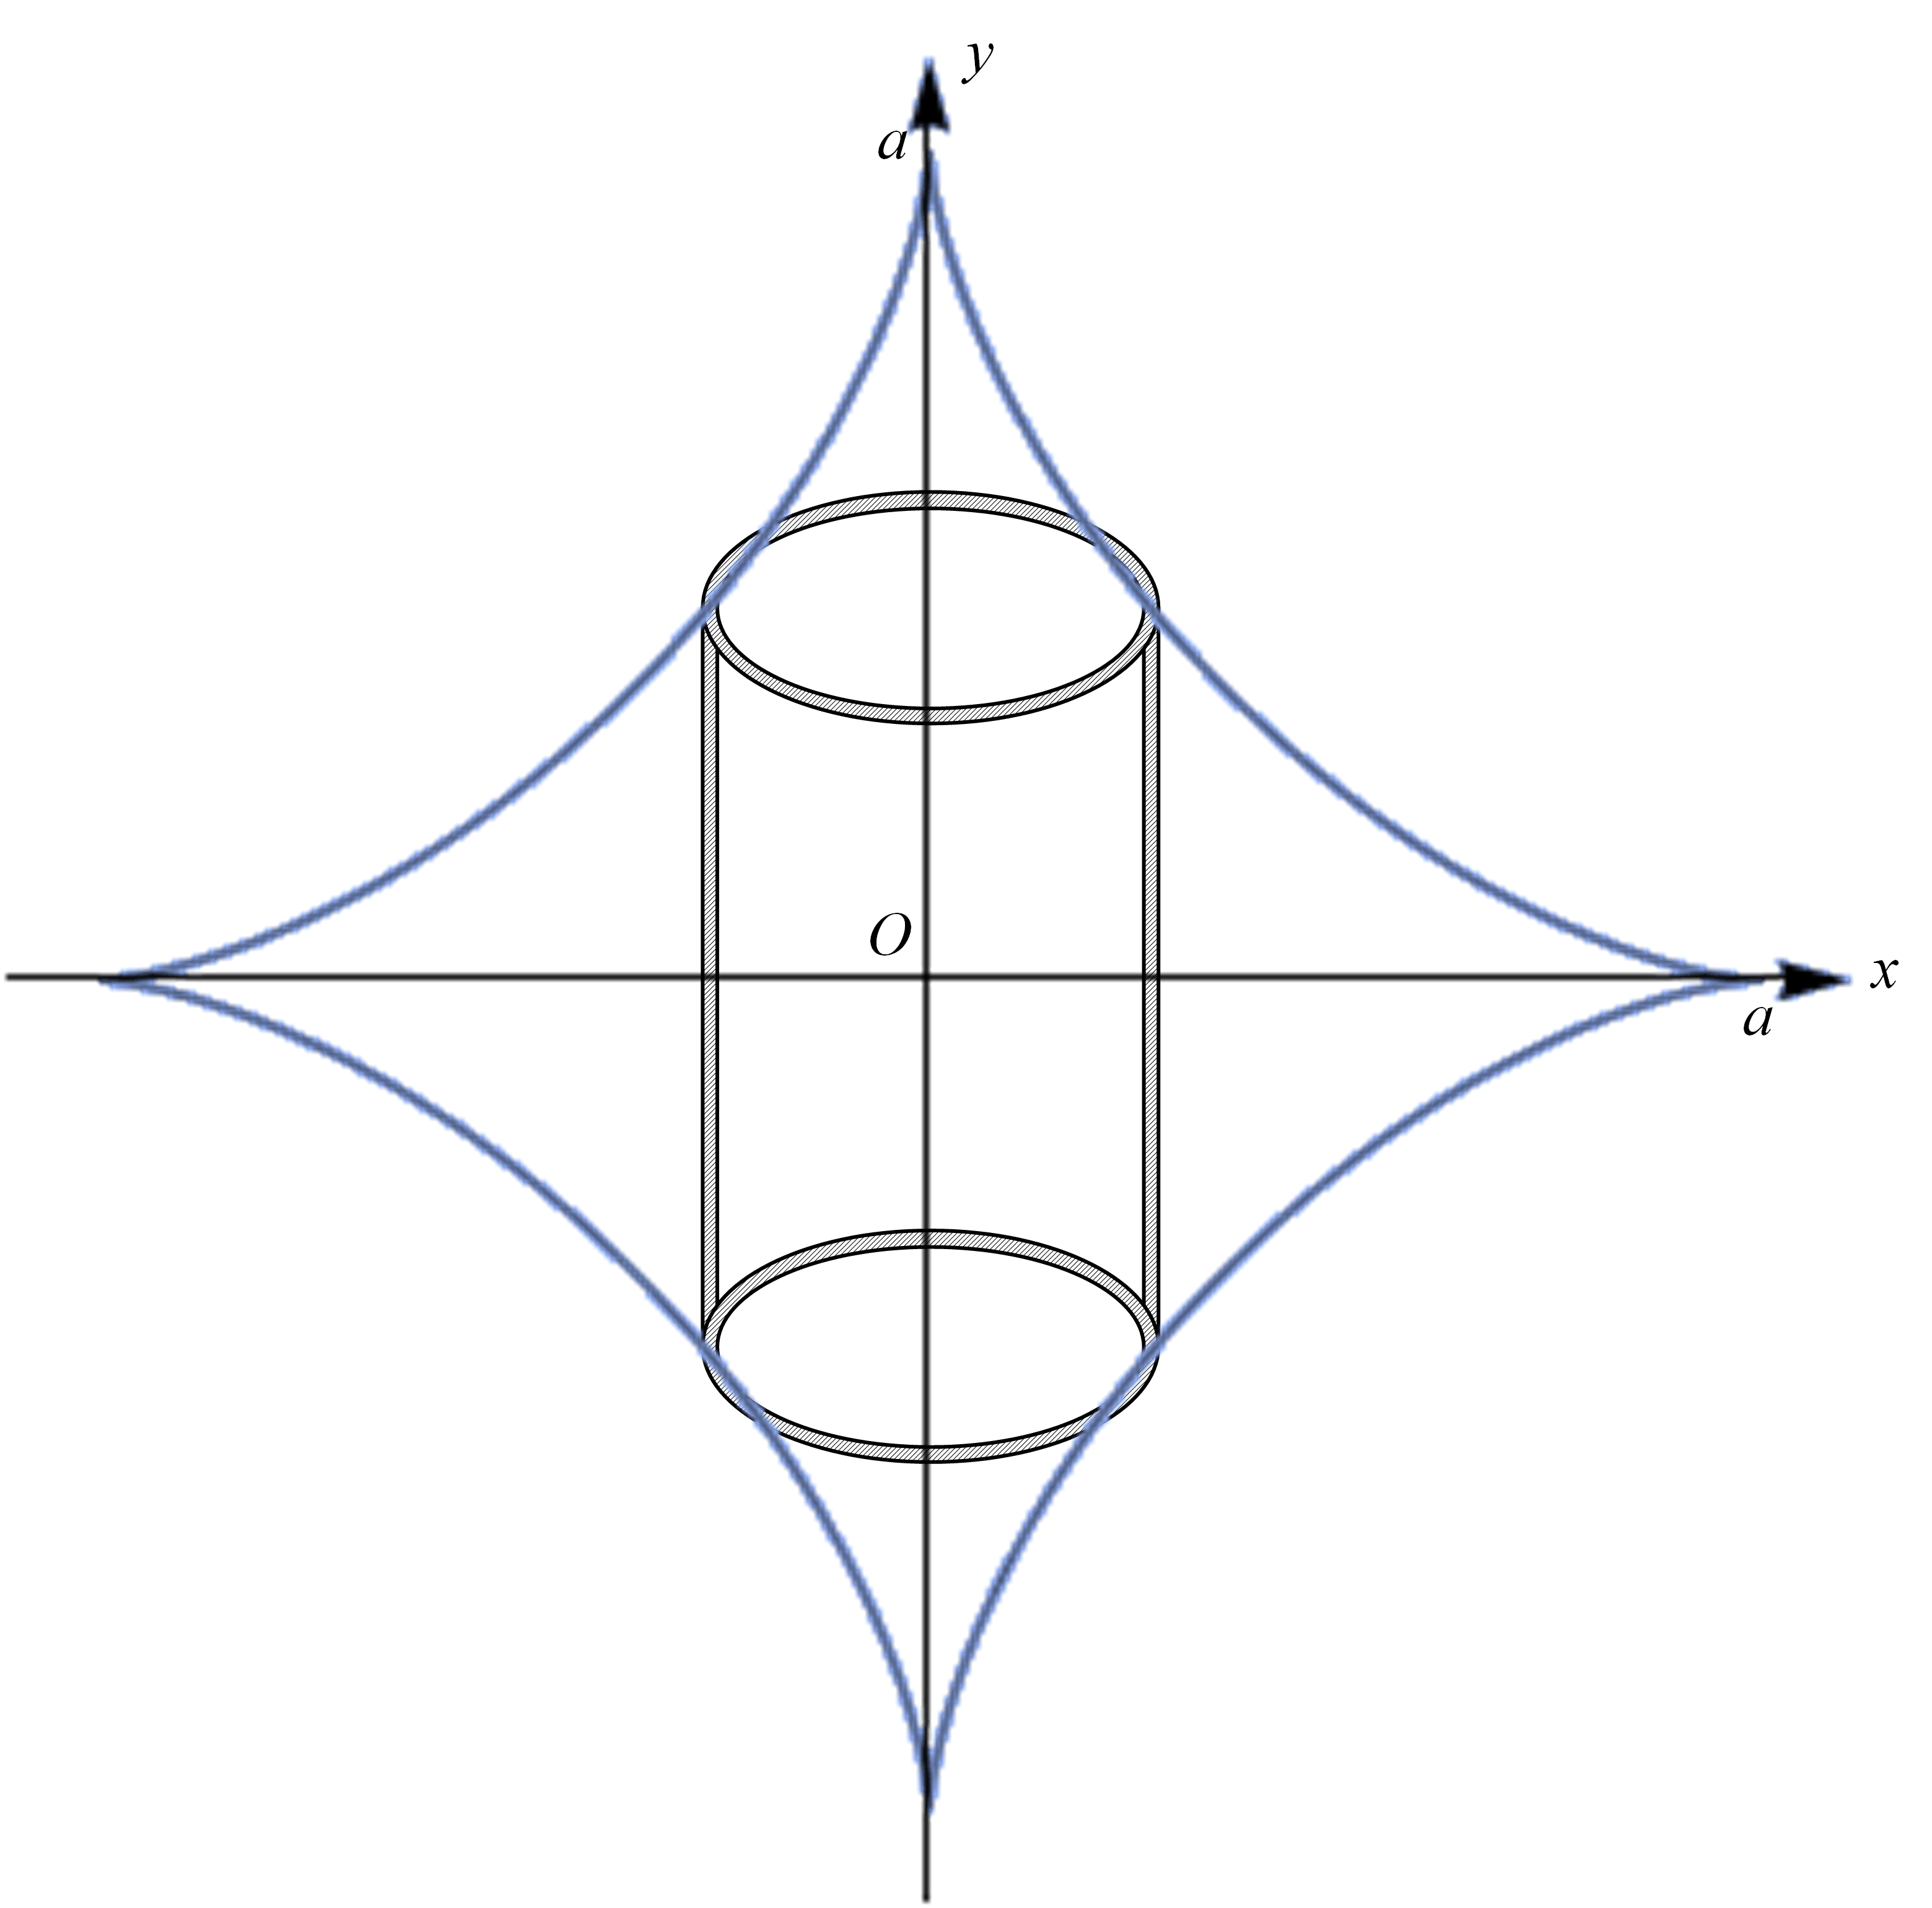
\includegraphics[height=0.3\textheight]{F:/life/2018AutumnTA/Exercises/11/Fig6-2-2.png} }}
%\begin{tabular}{cc}
%\includegraphics[height=0.3\textheight]{Fig6-2.png}
%&\includegraphics[height=0.3\textheight]{Fig6-2-3D.png}
%\end{tabular}
\end{center}
\caption{6.(2)题图示}
\end{figure}
(3)曲线形状如图~\ref{6-3-a}所示,绕$x$轴转动后得到的旋转体如图~\ref{6-3-b}所示. 设曲线最左侧的两点的横坐标为$x_0$,其中在$x$轴上方的点对应的极角为$\theta_0$,这两点将曲线分成黑色和红色的两部分,该旋转体可视为图~\ref{6-3-c}中的黑色轮廓绕$x$轴转动得到的旋转体剪去红色轮廓绕$x$轴转动得到的旋转体.

黑色轮廓绕$x$轴转动得到的旋转体的体积为
\[\begin{split}
V_1=\int_{x_0}^{2a}\pi y^2\mathrm dx=\int_{\theta_0}^0\pi[a(1+\cos\theta)\sin\theta]^2\mathrm d[a(1+\cos\theta)\cos\theta]
\end{split}\]
红色轮廓绕$x$轴转动得到的旋转体的体积为
\[\begin{split}
V_2=\int_{x_0}^{0}\pi y^2\mathrm dx=\int_{\theta_0}^\pi\pi[a(1+\cos\theta)\sin\theta]^2\mathrm d[a(1+\cos\theta)\cos\theta]
\end{split}\]
则原曲线绕$x$轴转动得到的旋转体的体积为
\[\begin{split}
V&=V_1-V_2\\
&=\int_{\theta_0}^0\pi[a(1+\cos\theta)\sin\theta]^2\mathrm d[a(1+\cos\theta)\cos\theta]-\int_{\theta_0}^\pi\pi[a(1+\cos\theta)\sin\theta]^2\mathrm d[a(1+\cos\theta)\cos\theta]\\
&=\int_{\theta_0}^0\pi[a(1+\cos\theta)\sin\theta]^2\mathrm d[a(1+\cos\theta)\cos\theta]+\int_\pi^{\theta_0}\pi[a(1+\cos\theta)\sin\theta]^2\mathrm d[a(1+\cos\theta)\cos\theta]\\
&=\int_\pi^0\pi[a(1+\cos\theta)\sin\theta]^2\mathrm d[a(1+\cos\theta)\cos\theta]\\
&=\pi a^2\int_\pi^0(1+\cos\theta)^2\sin^2\theta(-\sin\theta-2\cos\theta\sin\theta)\mathrm d\theta\\
&=\pi a^2\int_\pi^0(1+\cos\theta)^2(1-\cos^2\theta)(1+2\cos\theta)\mathrm d\cos\theta\\
&=\pi a^2\int_{-1}^1(1+u)^2(1-u^2)(1+2u)\mathrm du\\
&=\pi a^2\int_{-1}^1(1+4u+4u^2-2u^3-5u^4-2u^5)\mathrm du\\
&=\pi a^2(u+2u^2+\frac43u^3-\frac12u^4-u^5-\frac13u^6)\Big|_{-1}^1\\
&=\pi a^2(2+0+\frac43\cdot2-0-2-0)\\
&=\frac83\pi a^3
\end{split}\]
\begin{figure}[H]
\begin{center}
\subfloat[]{\label{6-3-a}
{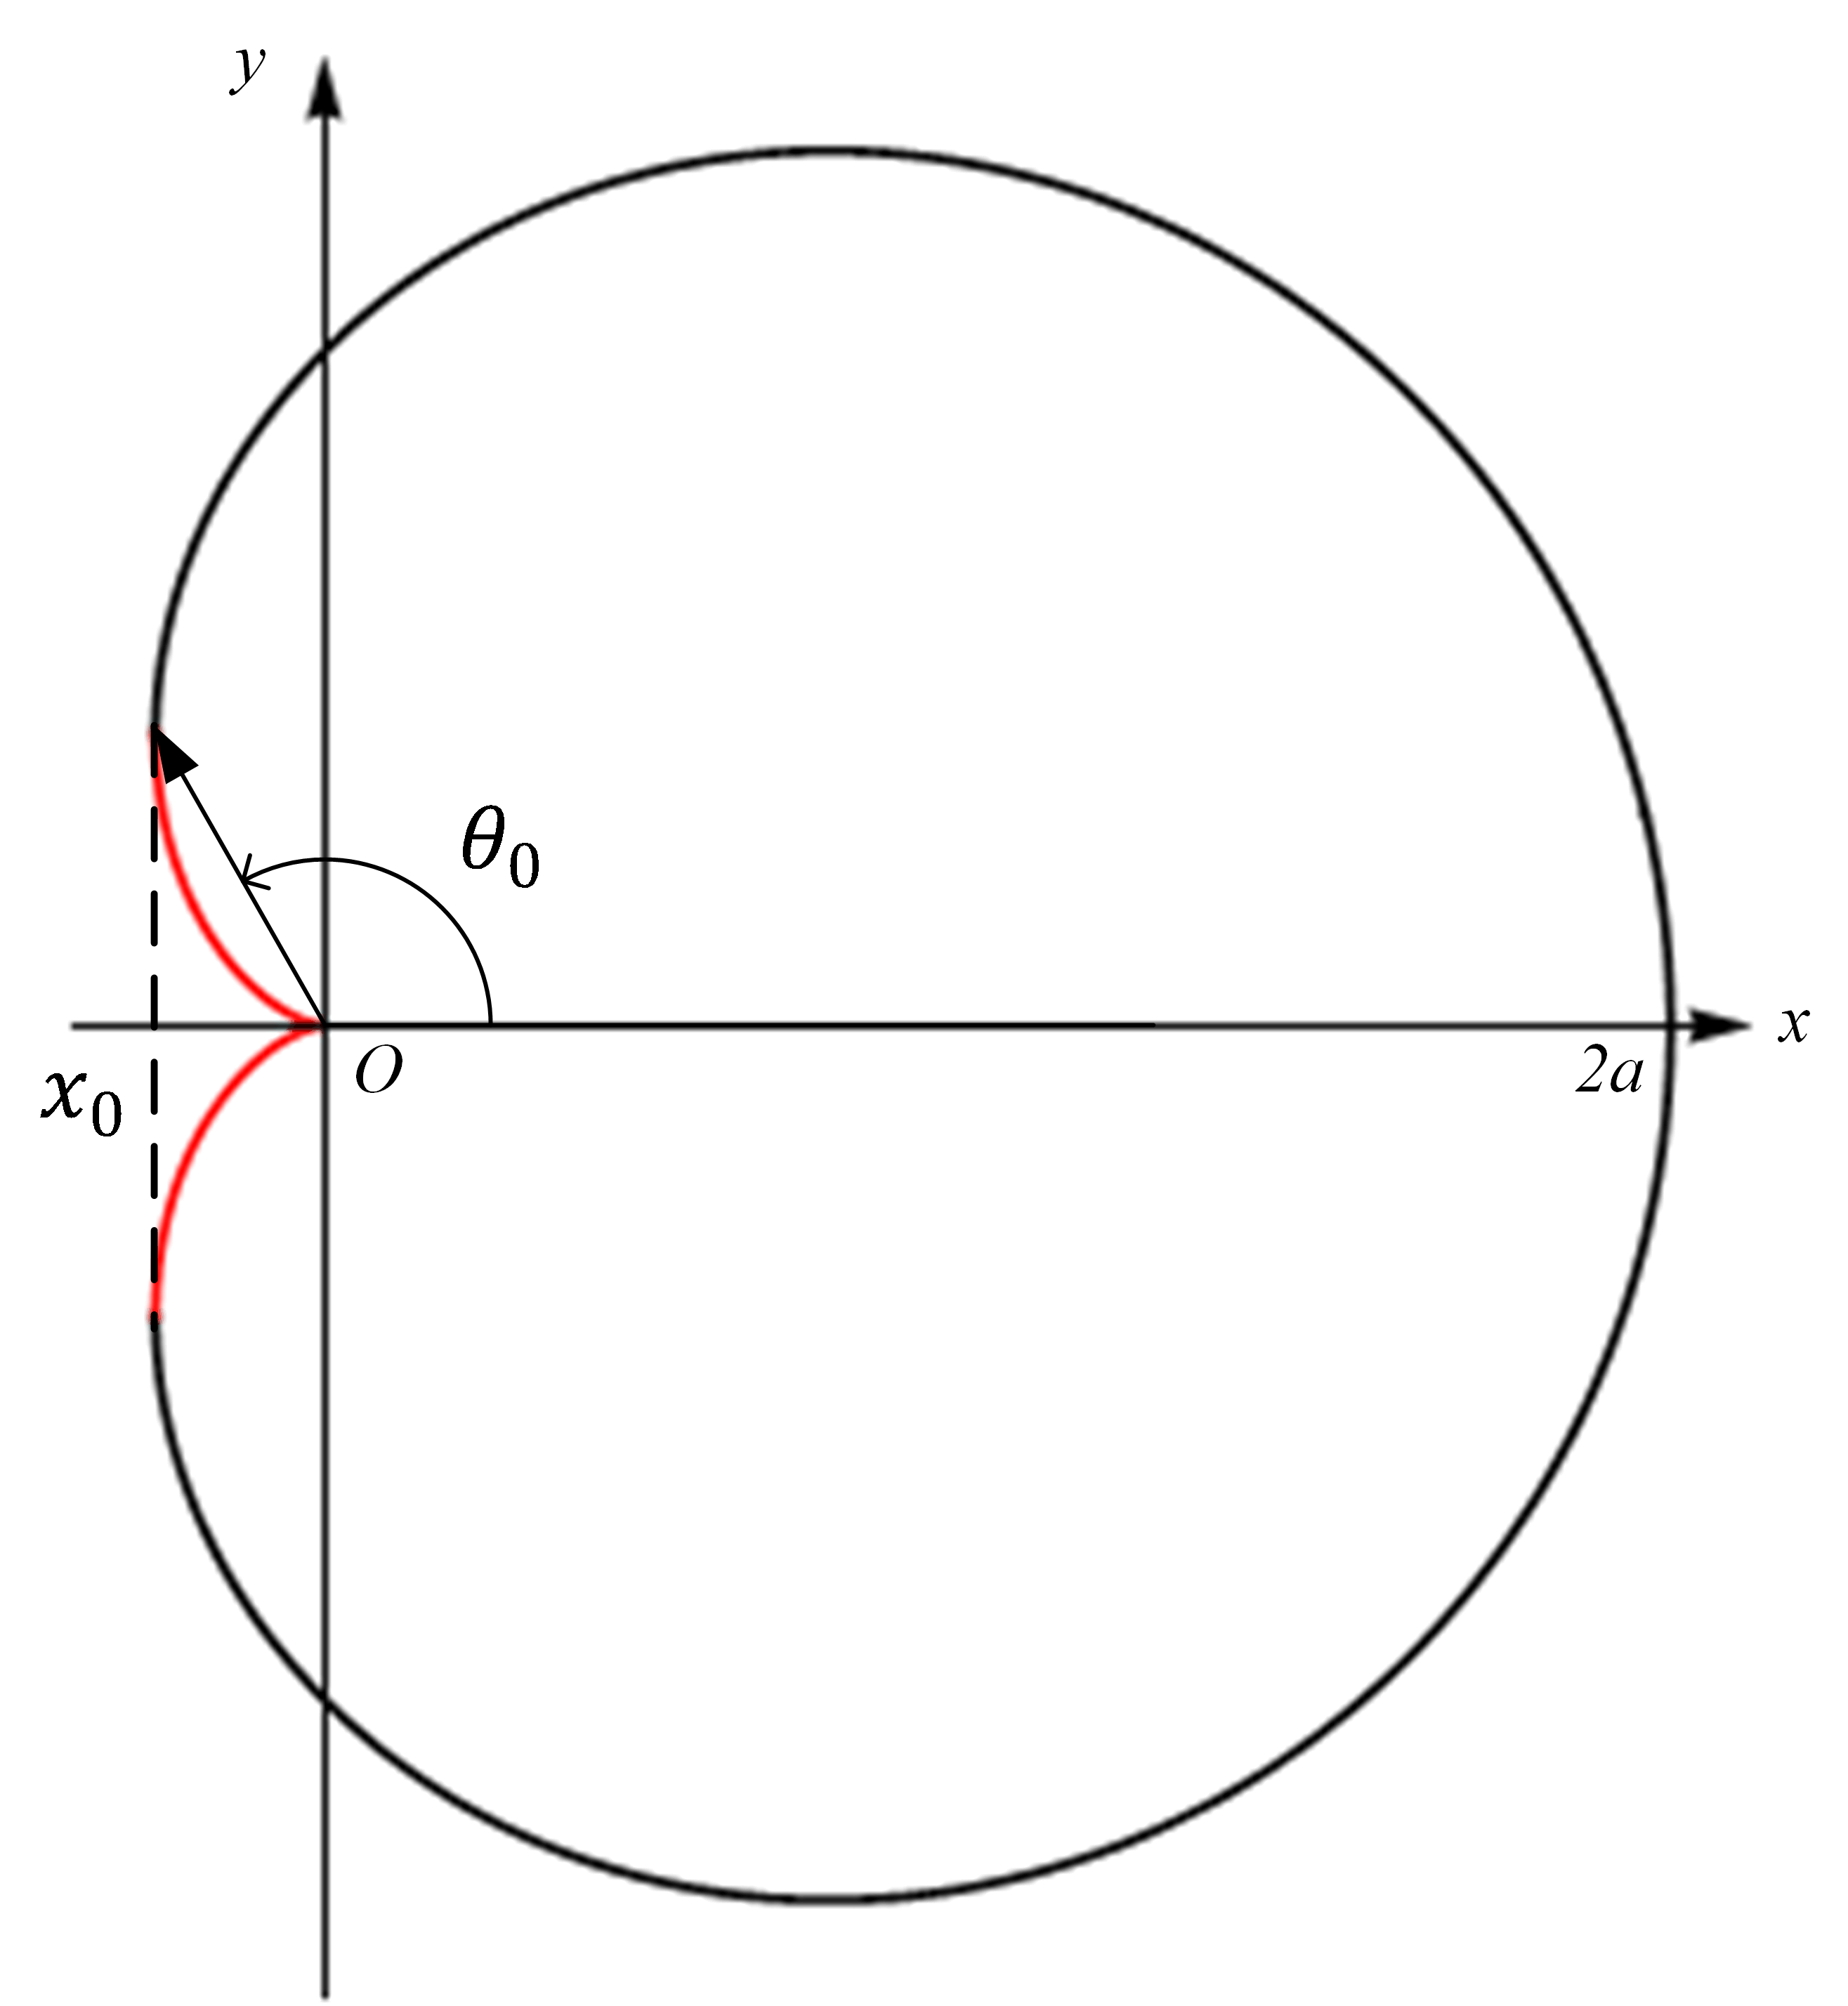
\includegraphics[height=0.3\textheight]{F:/life/2018AutumnTA/Exercises/11/Fig6-3.png} }}
    \subfloat[]{\label{6-3-b} {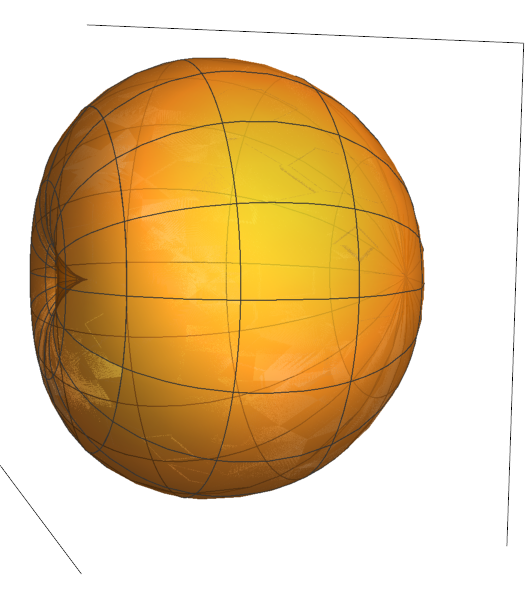
\includegraphics[height=0.3\textheight]{F:/life/2018AutumnTA/Exercises/11/Fig6-3-3D.png} }}\\
    \subfloat[]{\label{6-3-c} {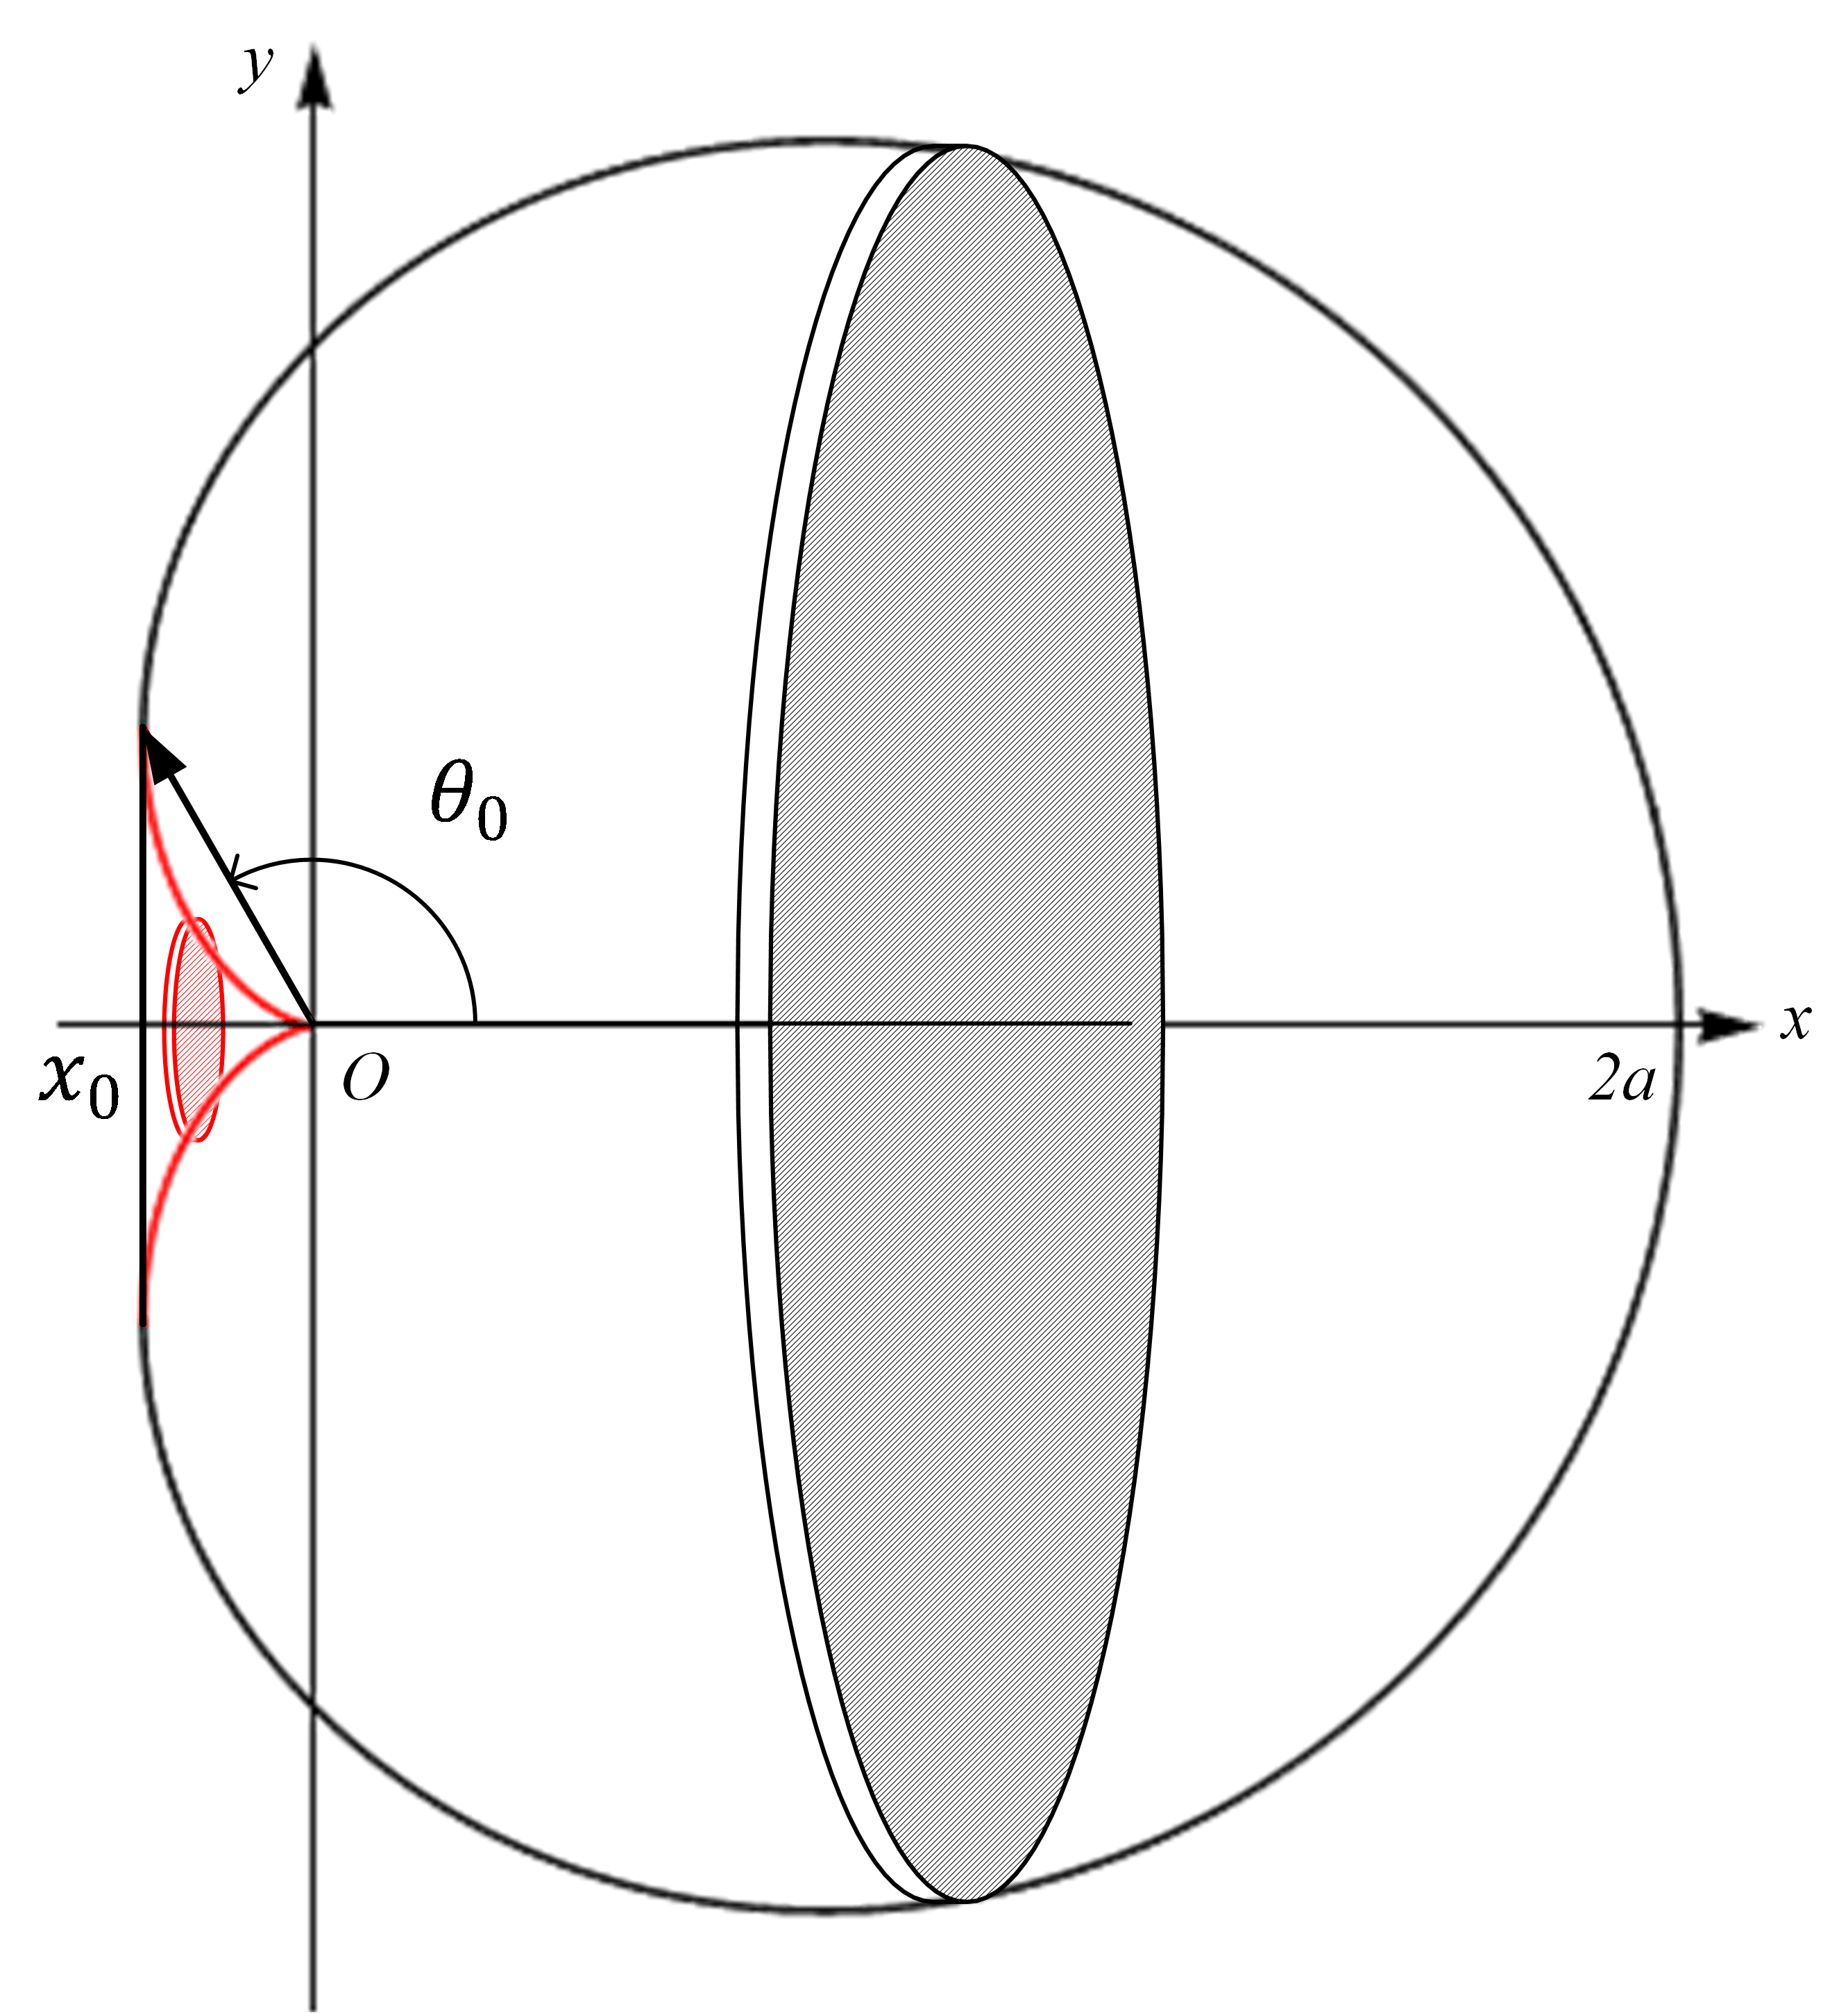
\includegraphics[height=0.3\textheight]{F:/life/2018AutumnTA/Exercises/11/Fig6-3-1.png} }}
\end{center}
\caption{6.(3)题图示}
\end{figure}
\item求下列旋转曲面的面积:
\newline
(1)$y^2=2px+a,0\leq x\leq a,a>1$绕$x$轴;
\newline
(2)$\begin{cases}
x=a(t-\sin t),\\
y=a(1-\cos t),
\end{cases}0\leq t\leq 2\pi$绕$x$轴.

解:(1)该旋转曲面的形状如图~\ref{5-7-1-2}所示,
\begin{figure}[H]
\begin{center}
\subfloat[]{\label{5-7-1-1}
{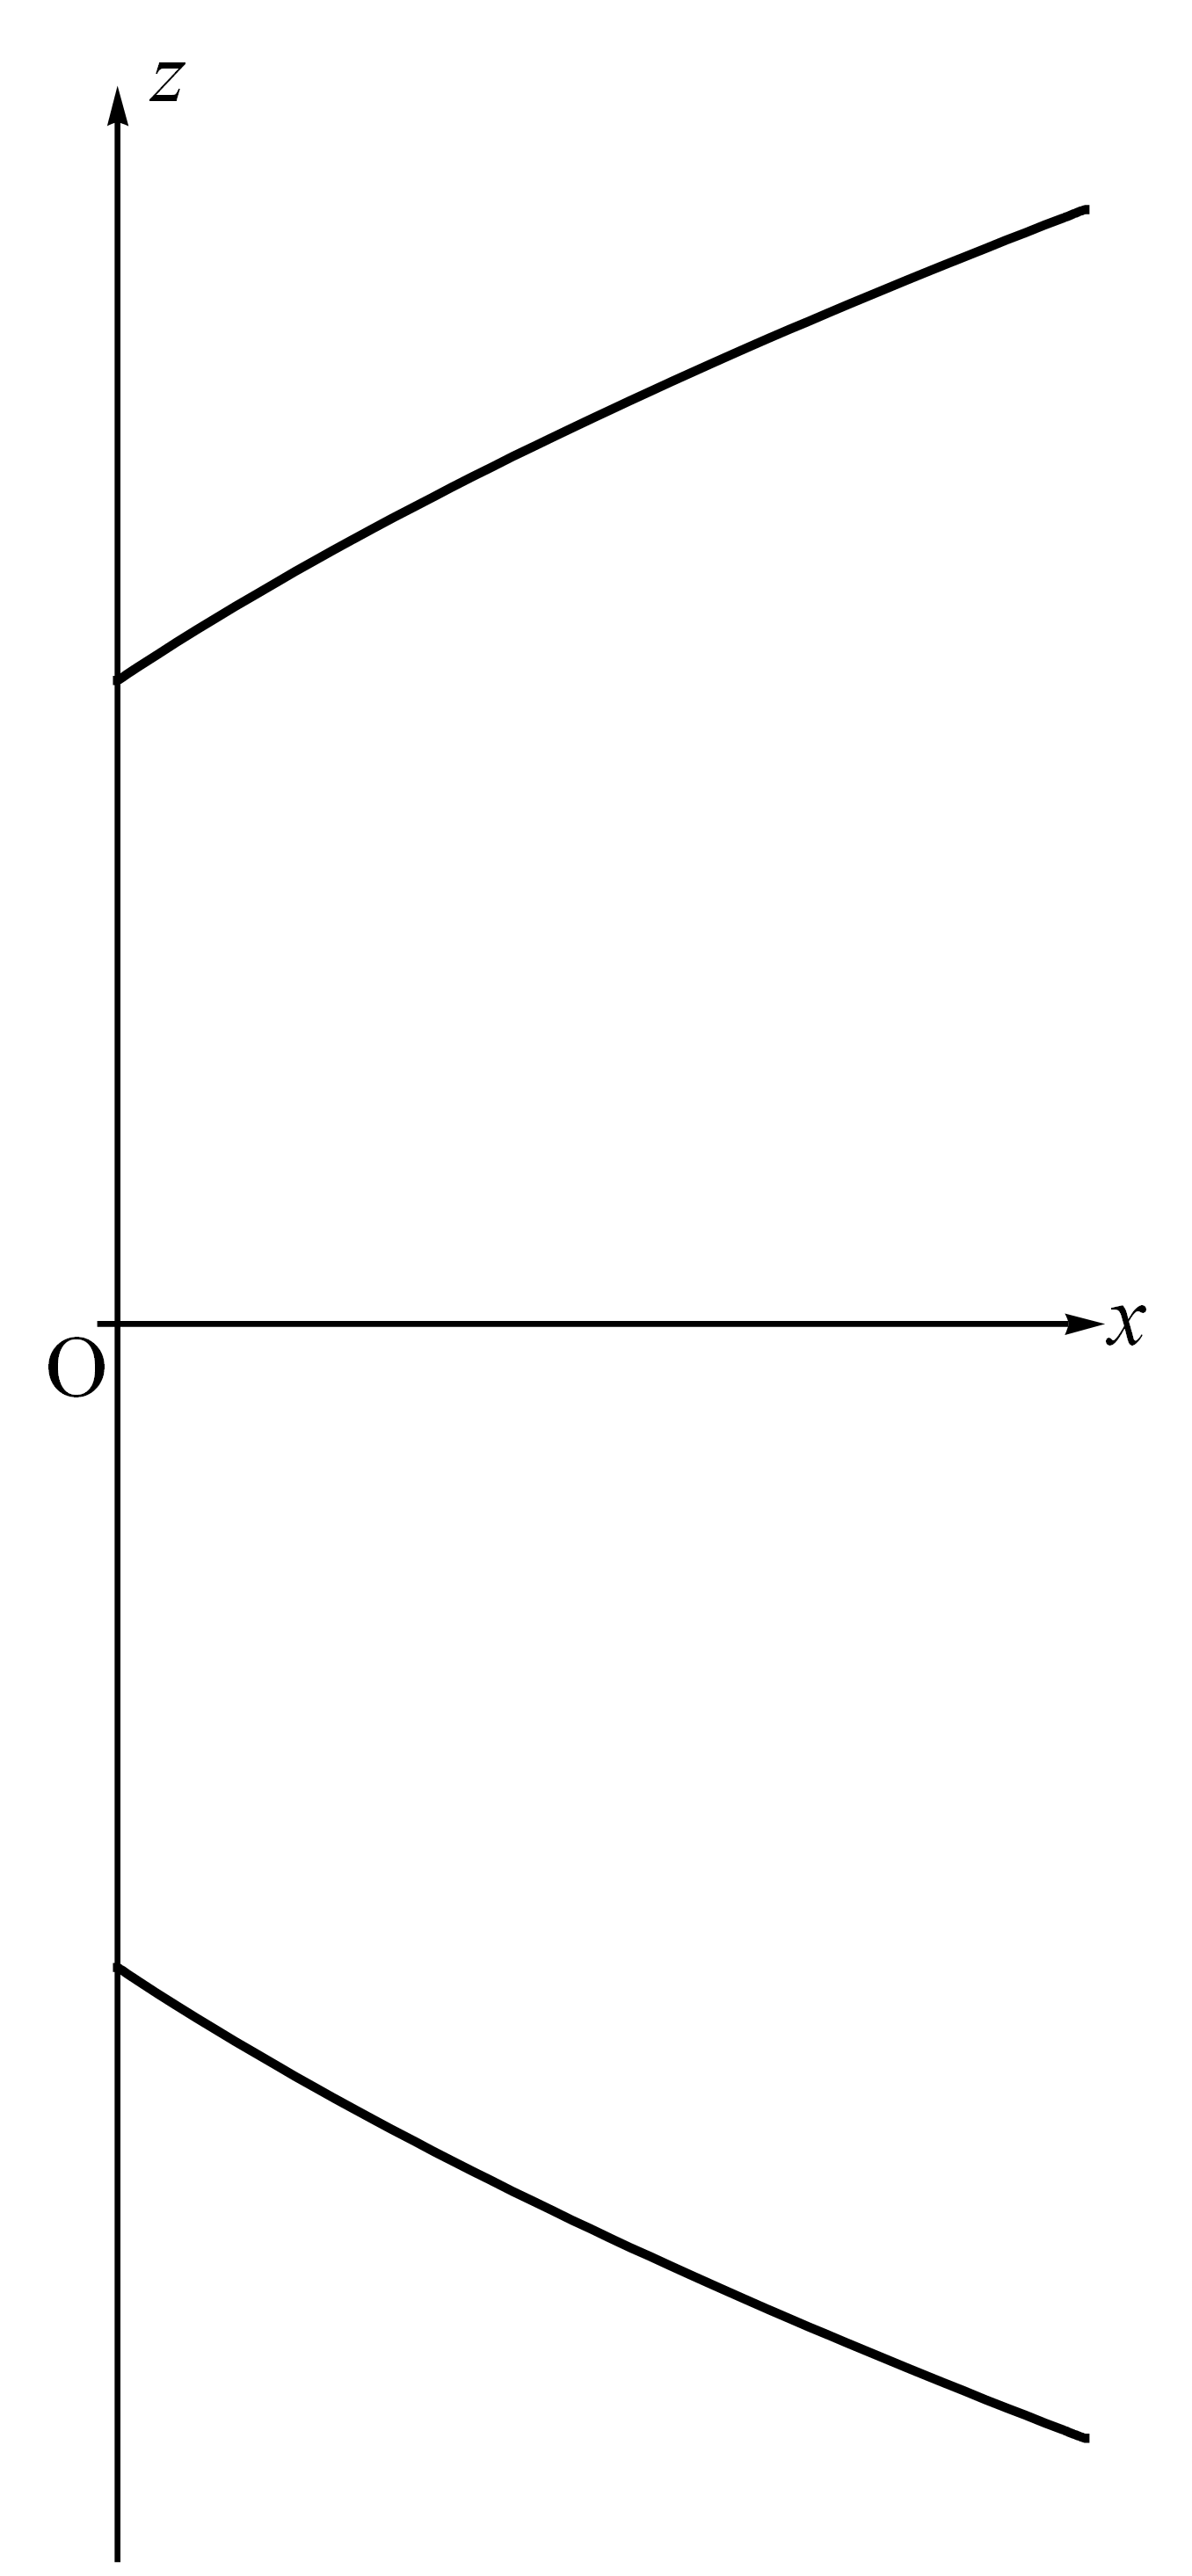
\includegraphics[height=0.3\textheight]{F:/life/2018AutumnTA/Exercises/11/Fig5-7-1-1.png} }}
    \subfloat[]{\label{5-7-1-2} {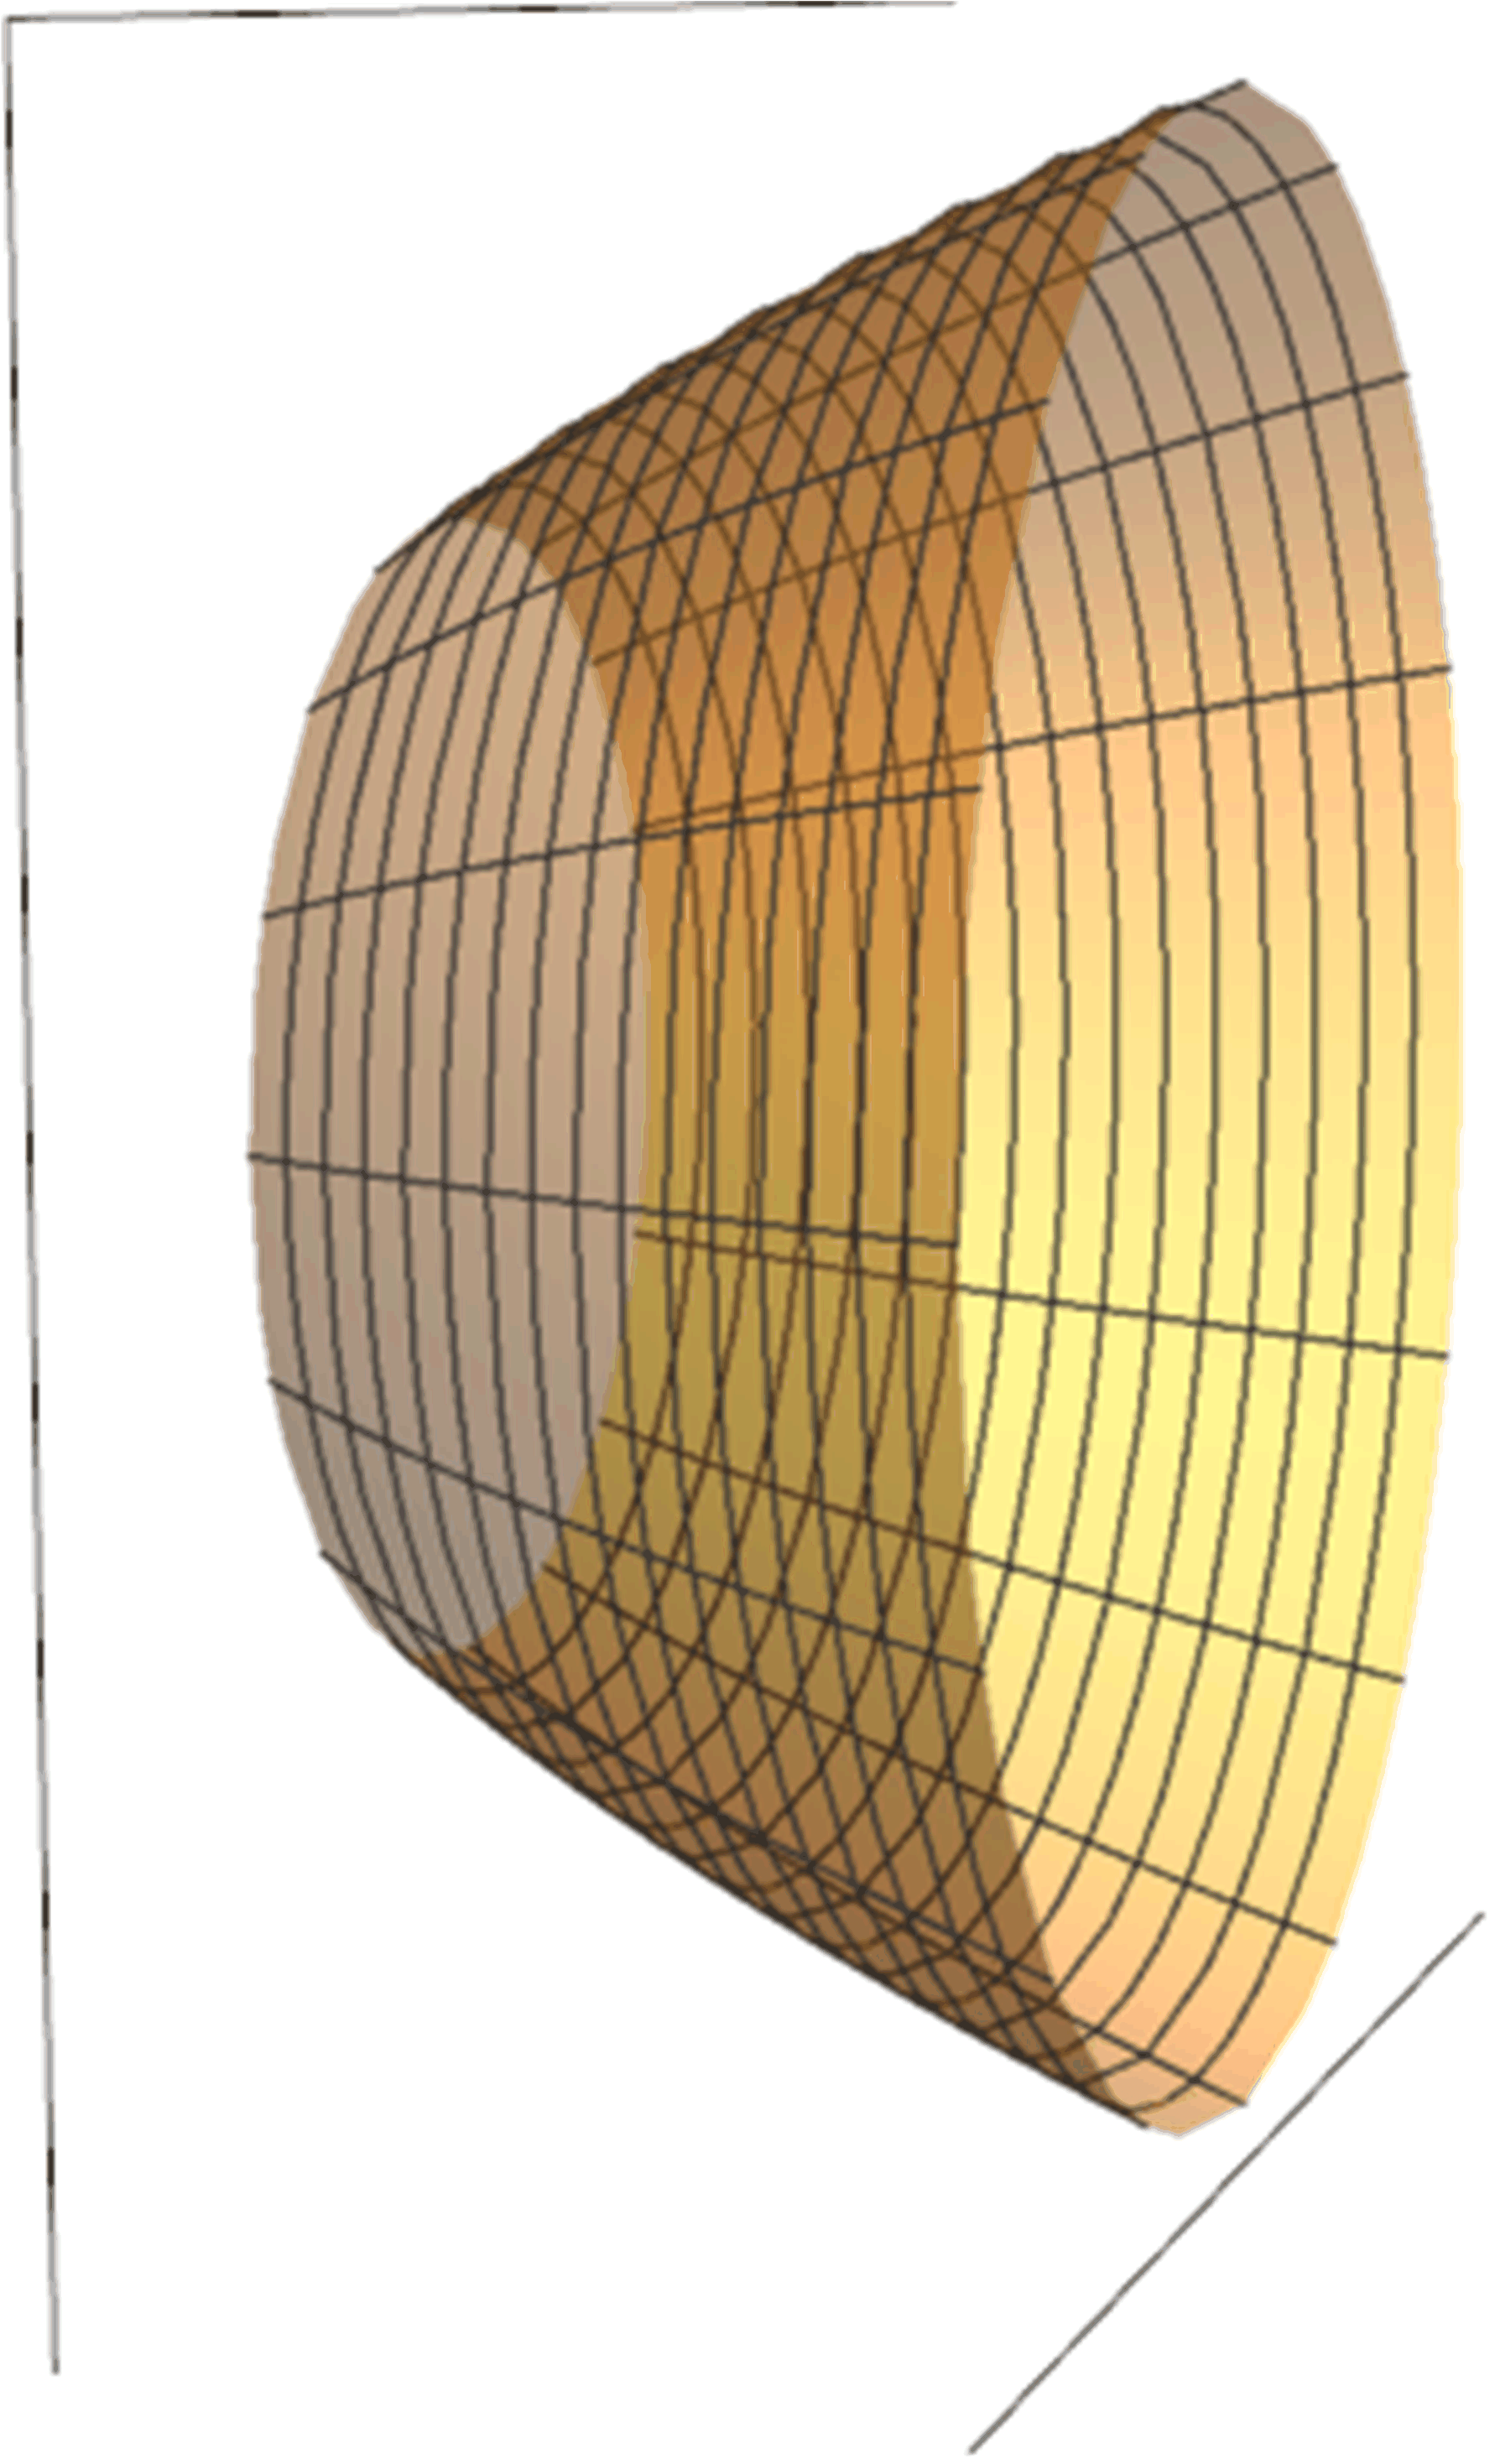
\includegraphics[height=0.3\textheight]{F:/life/2018AutumnTA/Exercises/11/Fig5-7-1-2.png} }}
    \subfloat[]{\label{5-7-1-3} {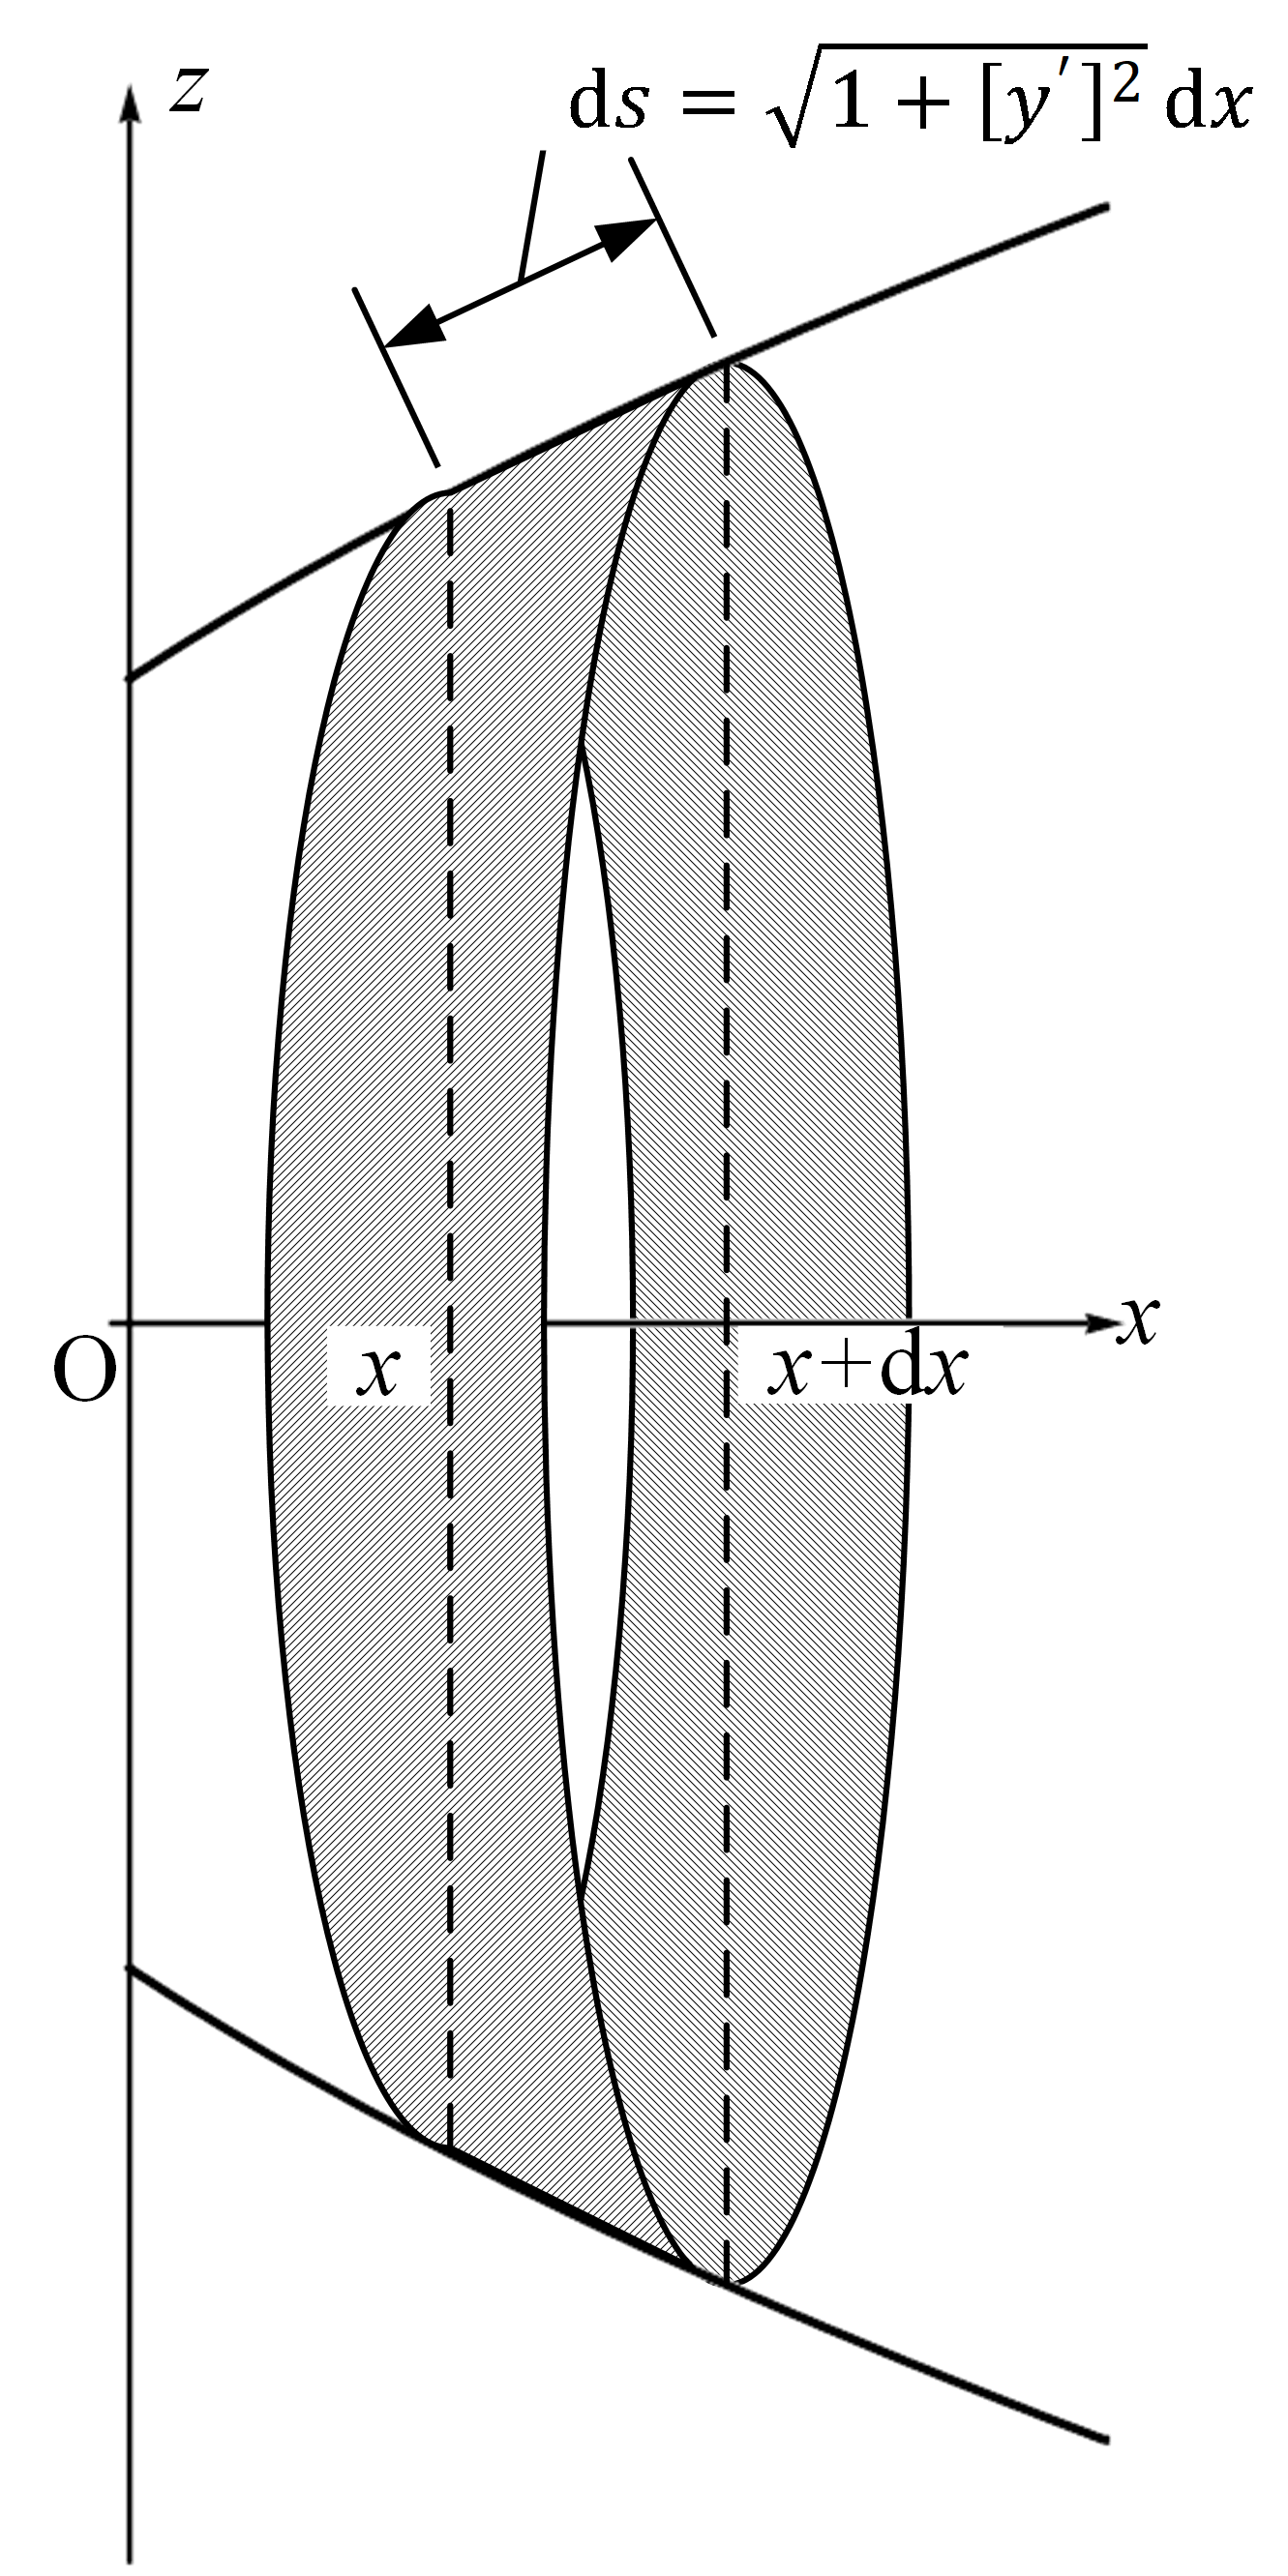
\includegraphics[height=0.3\textheight]{F:/life/2018AutumnTA/Exercises/11/Fig5-7-1-3.png} }}
\end{center}
\caption{7.(1)题图示}
\label{5-7-1}
\end{figure}
取如图~\ref{5-7-1-3}所示的曲面元,当$y>0$时,将$y^2=2px+a$两侧对$x$求导得$2yy'=2p,y'=\frac py$,则该旋转曲面的面积
\[\begin{split}
S&=\int_0^a2\pi y(x)\sqrt{1+[y'(x)]^2}\mathrm dx=\int_0^a2\pi y\sqrt{1+(\frac py)^2}\mathrm dx=2\pi\int_0^a\sqrt{y^2+p^2}\mathrm dx\\
&=2\int_0^a\sqrt{2px+a+p^2}\mathrm dx=\frac{2\pi}{2p}\frac23(2px+a+p^2)^{\frac32}\Big|_0^a\\
&=\frac{2\pi}{3p}(2pa+a+p^2)^{\frac32}-\frac{2\pi}{3p}(a+p^2)^{\frac32}.
\end{split}\]

(2)该旋转曲面的形状如图~\ref{5-7-2-2}所示,
\begin{figure}[H]
\begin{center}
\subfloat[]{\label{5-7-2-1}
{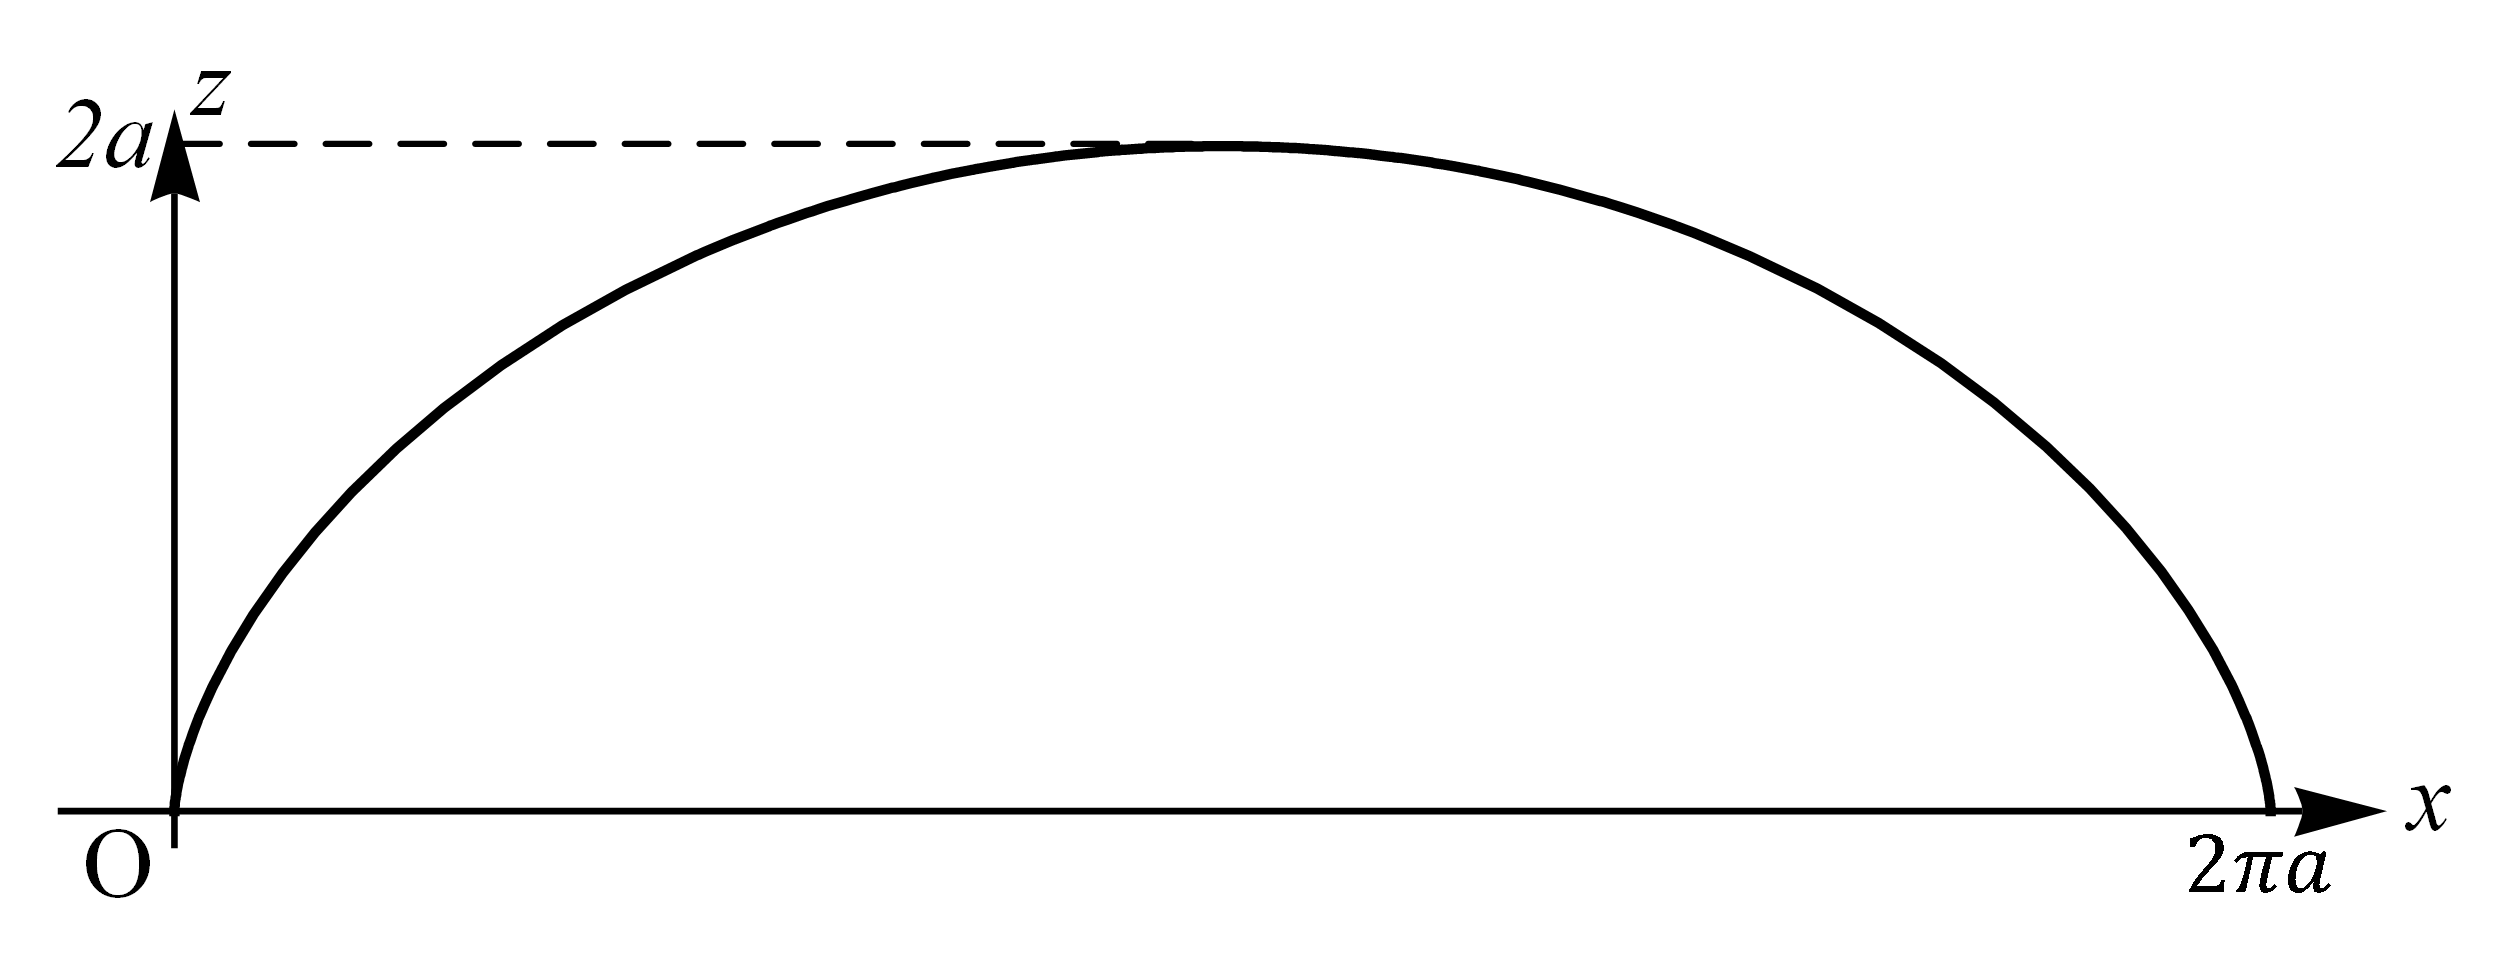
\includegraphics[height=0.15\textheight]{F:/life/2018AutumnTA/Exercises/11/Fig5-7-2-1.png} }}
    \subfloat[]{\label{5-7-2-2} {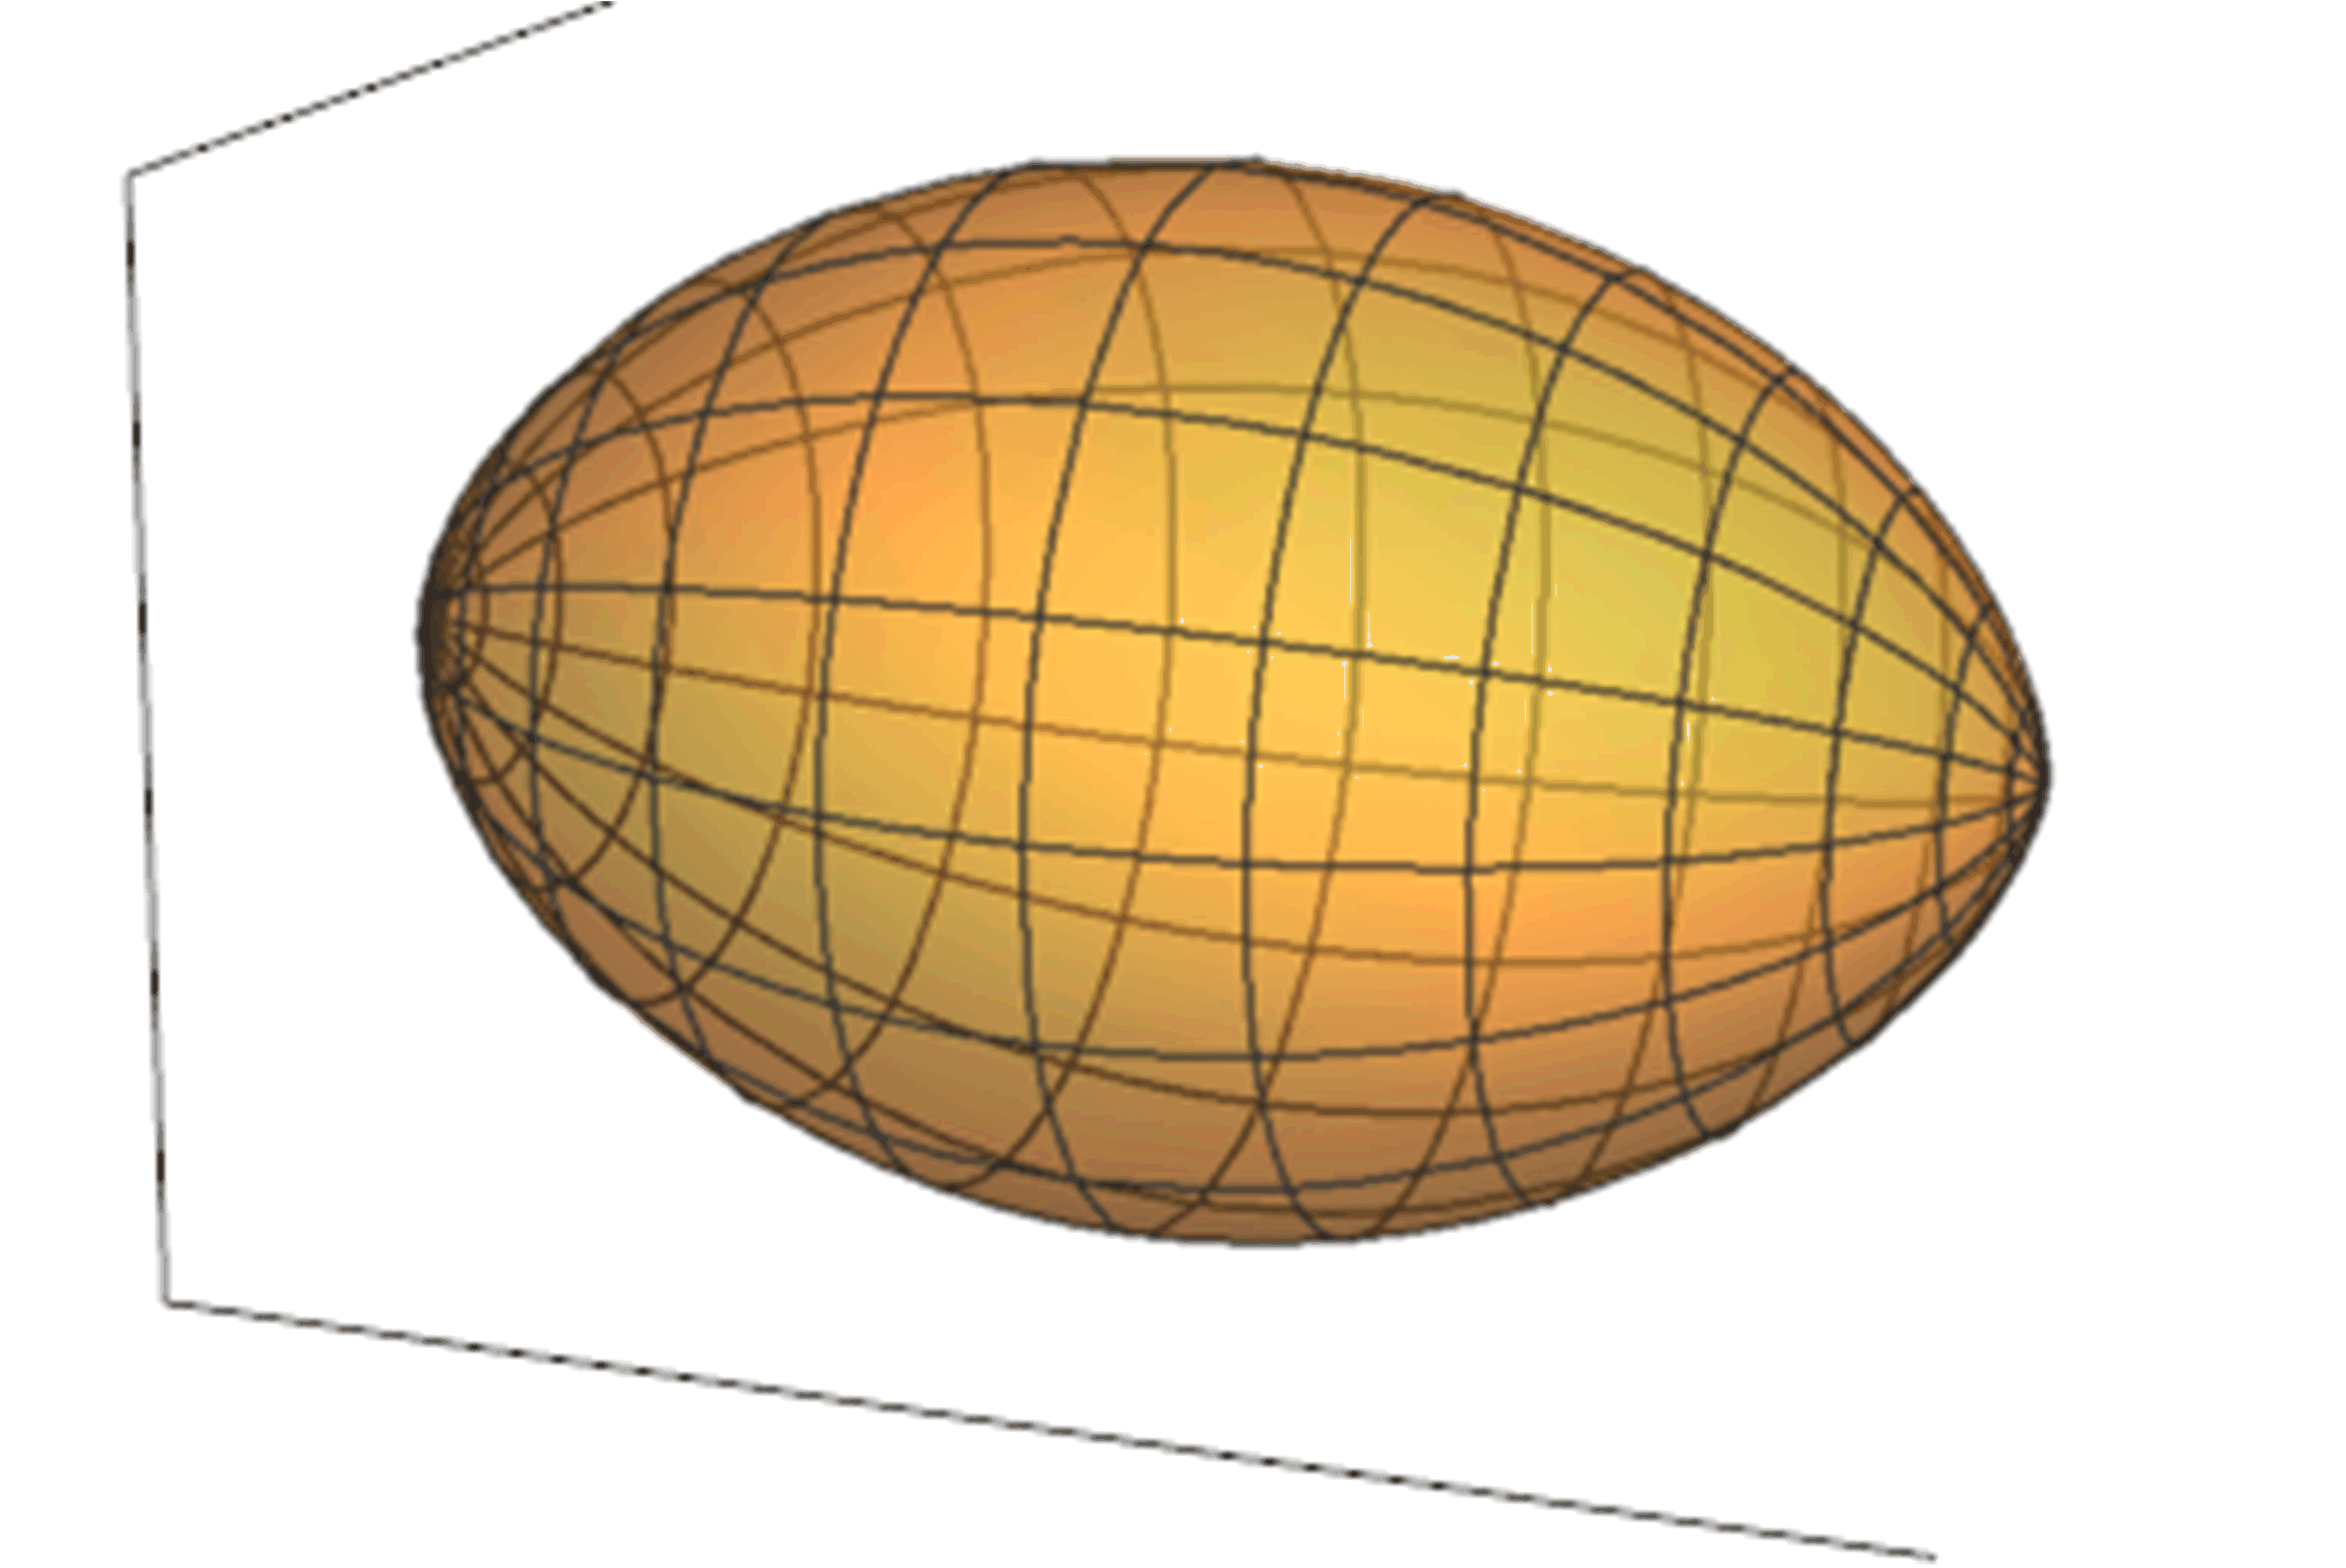
\includegraphics[height=0.25\textheight]{F:/life/2018AutumnTA/Exercises/11/Fig5-7-2-2.png} }}\\
    \subfloat[]{\label{5-7-2-3} {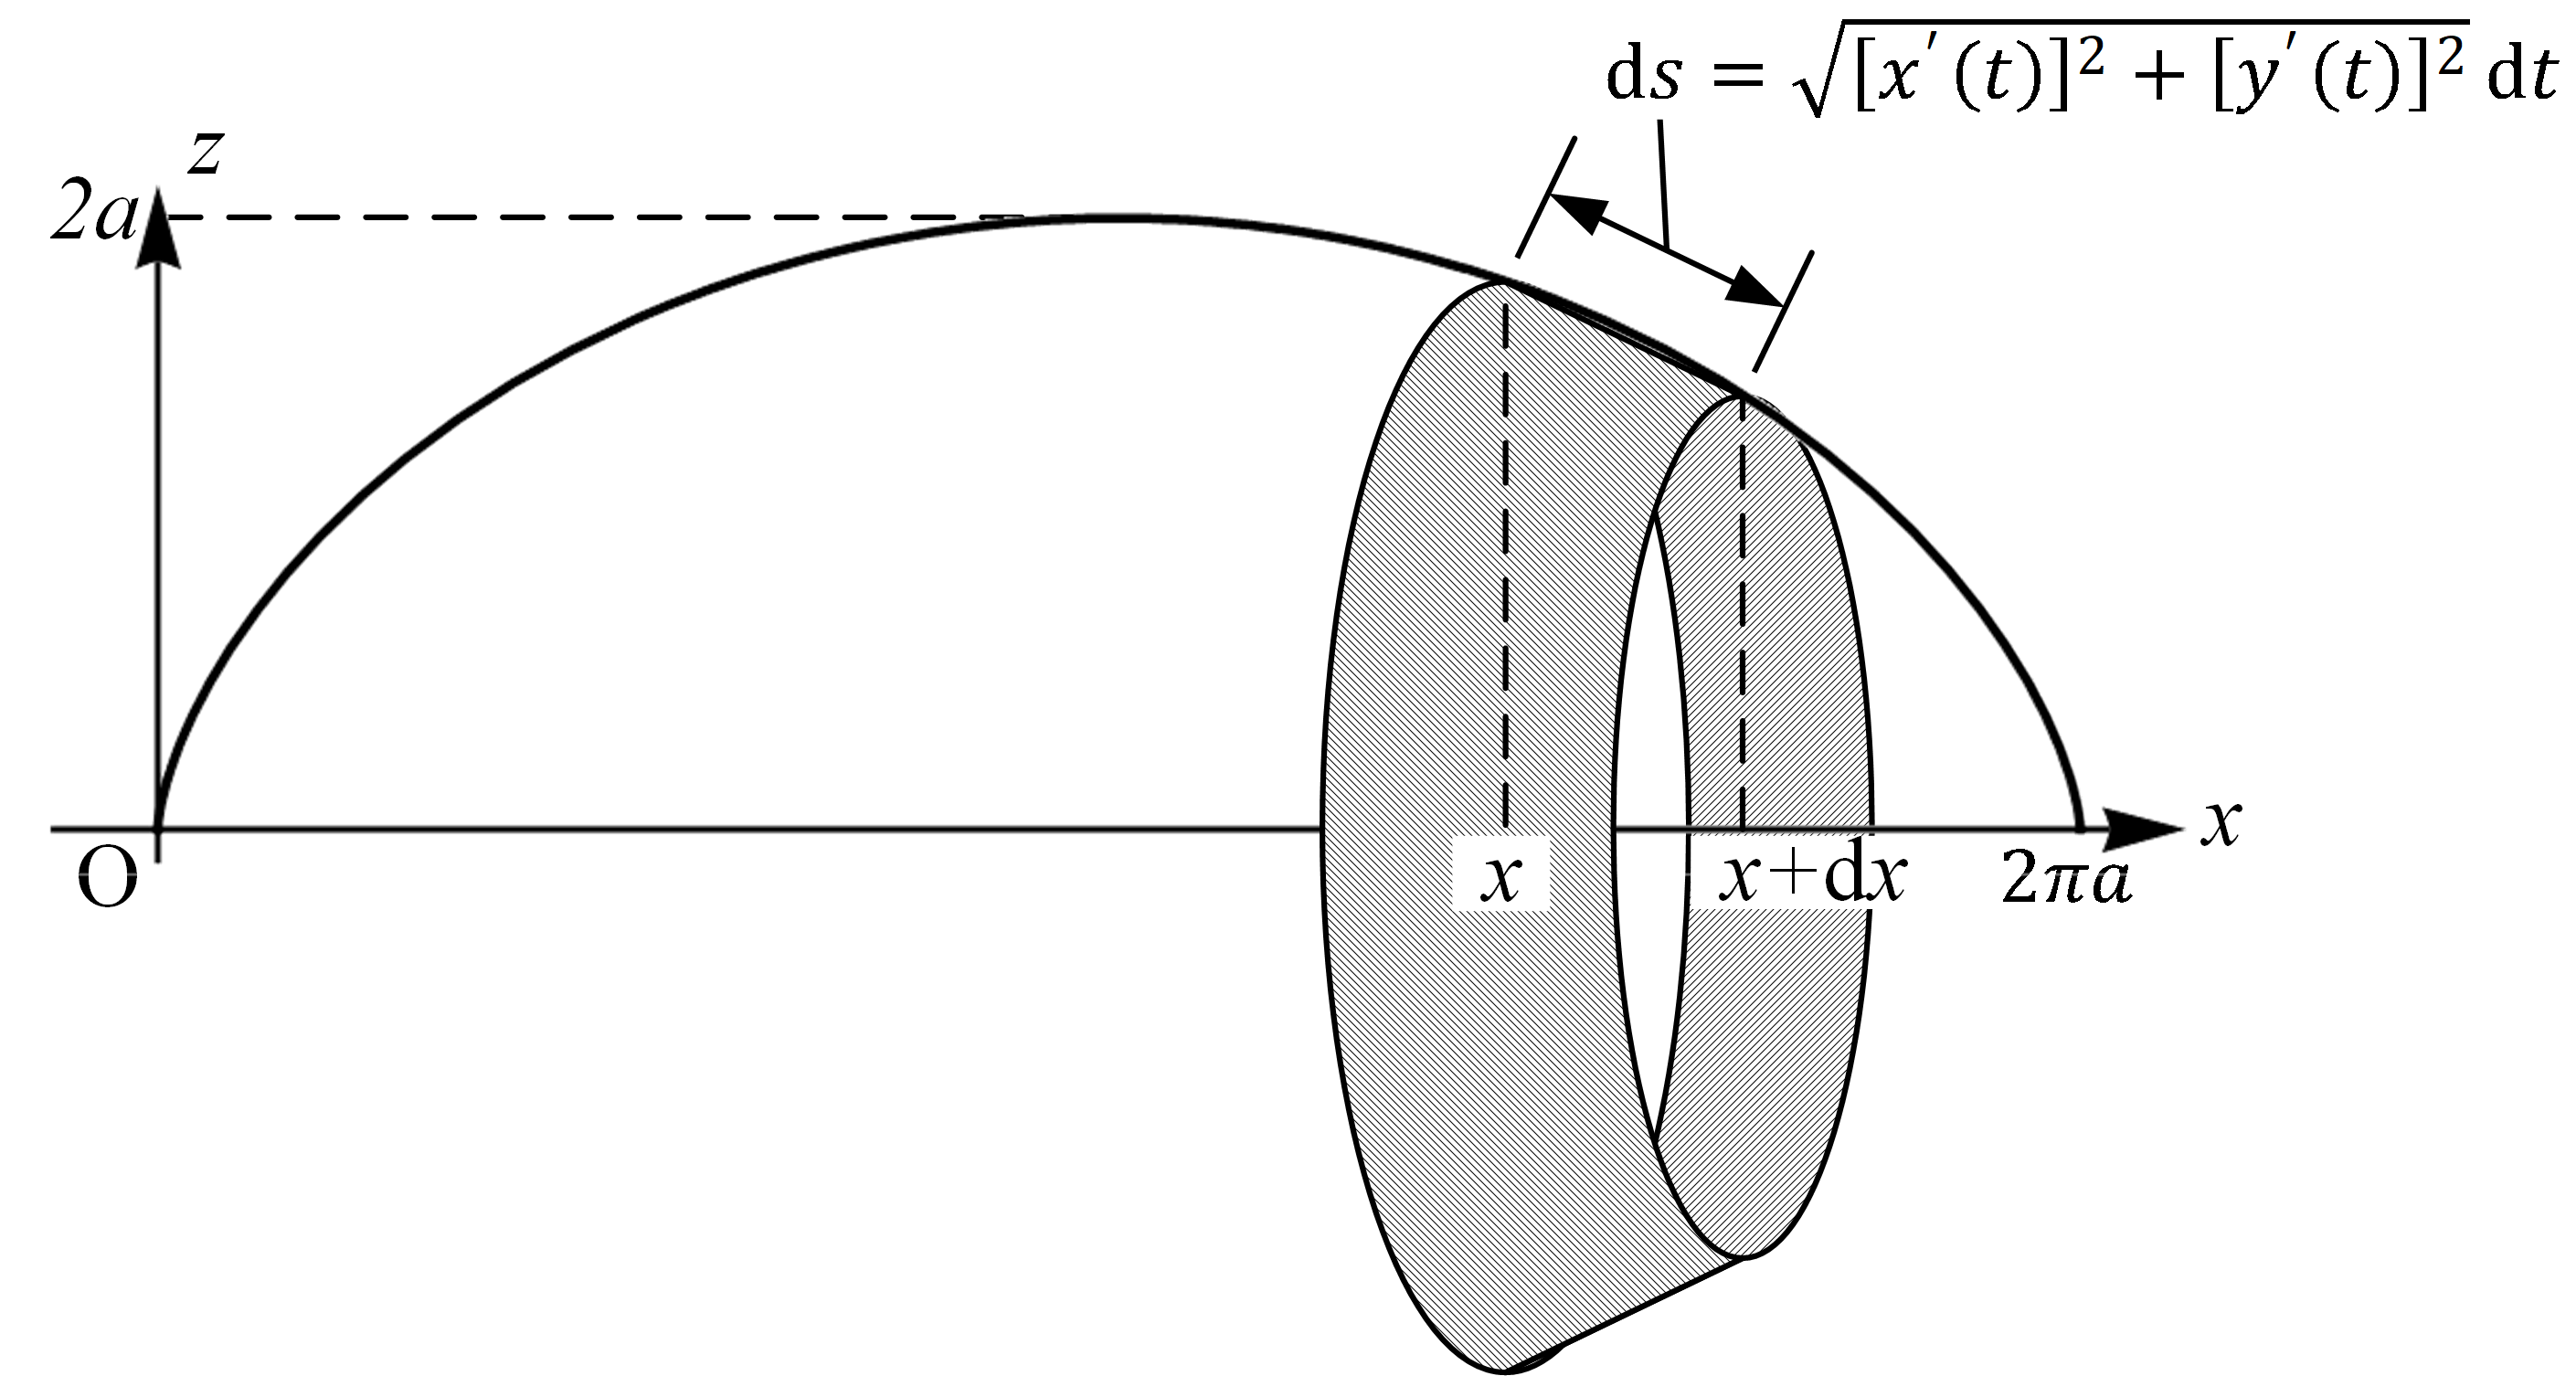
\includegraphics[height=0.25\textheight]{F:/life/2018AutumnTA/Exercises/11/Fig5-7-2-3.png} }}
\end{center}
\caption{7.(2)题图示}
\label{5-7-2}
\end{figure}
取曲面元如图~\ref{5-7-2-3}所示,当$0\leq t\leq 2\pi$时$x\geq0,y\geq0$,曲面面积
\[\begin{split}
S&=\int_0^{2\pi}2\pi y(t)\sqrt{[x'(t)]^2[(y'(t)]^2}\mathrm dt=\int_0^{2\pi}2\pi a(1-\cos t)\sqrt{a^2(1-\cos t)^2+a^2(\sin t)^2}\mathrm dt\\
&=2\pi a^2\int_0^{2\pi}(1-\cos t)\sqrt{2-2\cos t}\mathrm dt=2\sqrt2\pi a^2\int_0^{2\pi}2\sin^2\frac t2|\sqrt2\sin\frac t2|\mathrm dt\\
&=8\pi a^2\int_0^{2\pi}\sin^3\frac t2\mathrm dt=-16\pi a^2\int_0^{2\pi}(1-\cos^2\frac t2)\mathrm d\cos\frac t2=-16\pi a^2(\cos\frac t2-\frac13\cos^3\frac t2)\Big|_0^{2\pi}\\
&=-16\pi a^2[(-1-1)-\frac13(-1-1)]=\frac{64}3\pi a^2.
\end{split}\]
\end{enumerate}
\subsection{习题7.6解答}
\begin{enumerate}
\item半径等于$r$的球沉入水中,与水面相切. 球体的质量密度与水相同. 现将球从水中取出,外力需要做多少功?

解:建立如图~\ref{7-6-1}所示的坐标系,因球体的质量密度与水相同,故图中的微元在水下提升过程中受到的重力和浮力平衡,将球从水中取出,只在水上提升的过程中克服微元的重力做功,外力做的总功
\[\begin{split}
W=&\int_{-r}^r(r+x)\rho\mathrm g\pi(r^2-x^2)\mathrm dx=\rho\mathrm g\pi\int_{-r}^r(r^3-rx^2+r^2x-x^3)\mathrm dx\\
=&\rho\mathrm g\pi(r^3x-\frac r3x^3+\frac{r^2}2x^2-\frac14x^4)\Big|_{-r}^r=\rho\mathrm g\pi[r^3(2r)-\frac r3(2r^3)+0+0]\\
=&\frac43\rho\mathrm g\pi r^4=\frac43\pi r^4(\text{取}\rho\mathrm g=1).
\end{split}\]

\begin{figure}[H]
\begin{center}
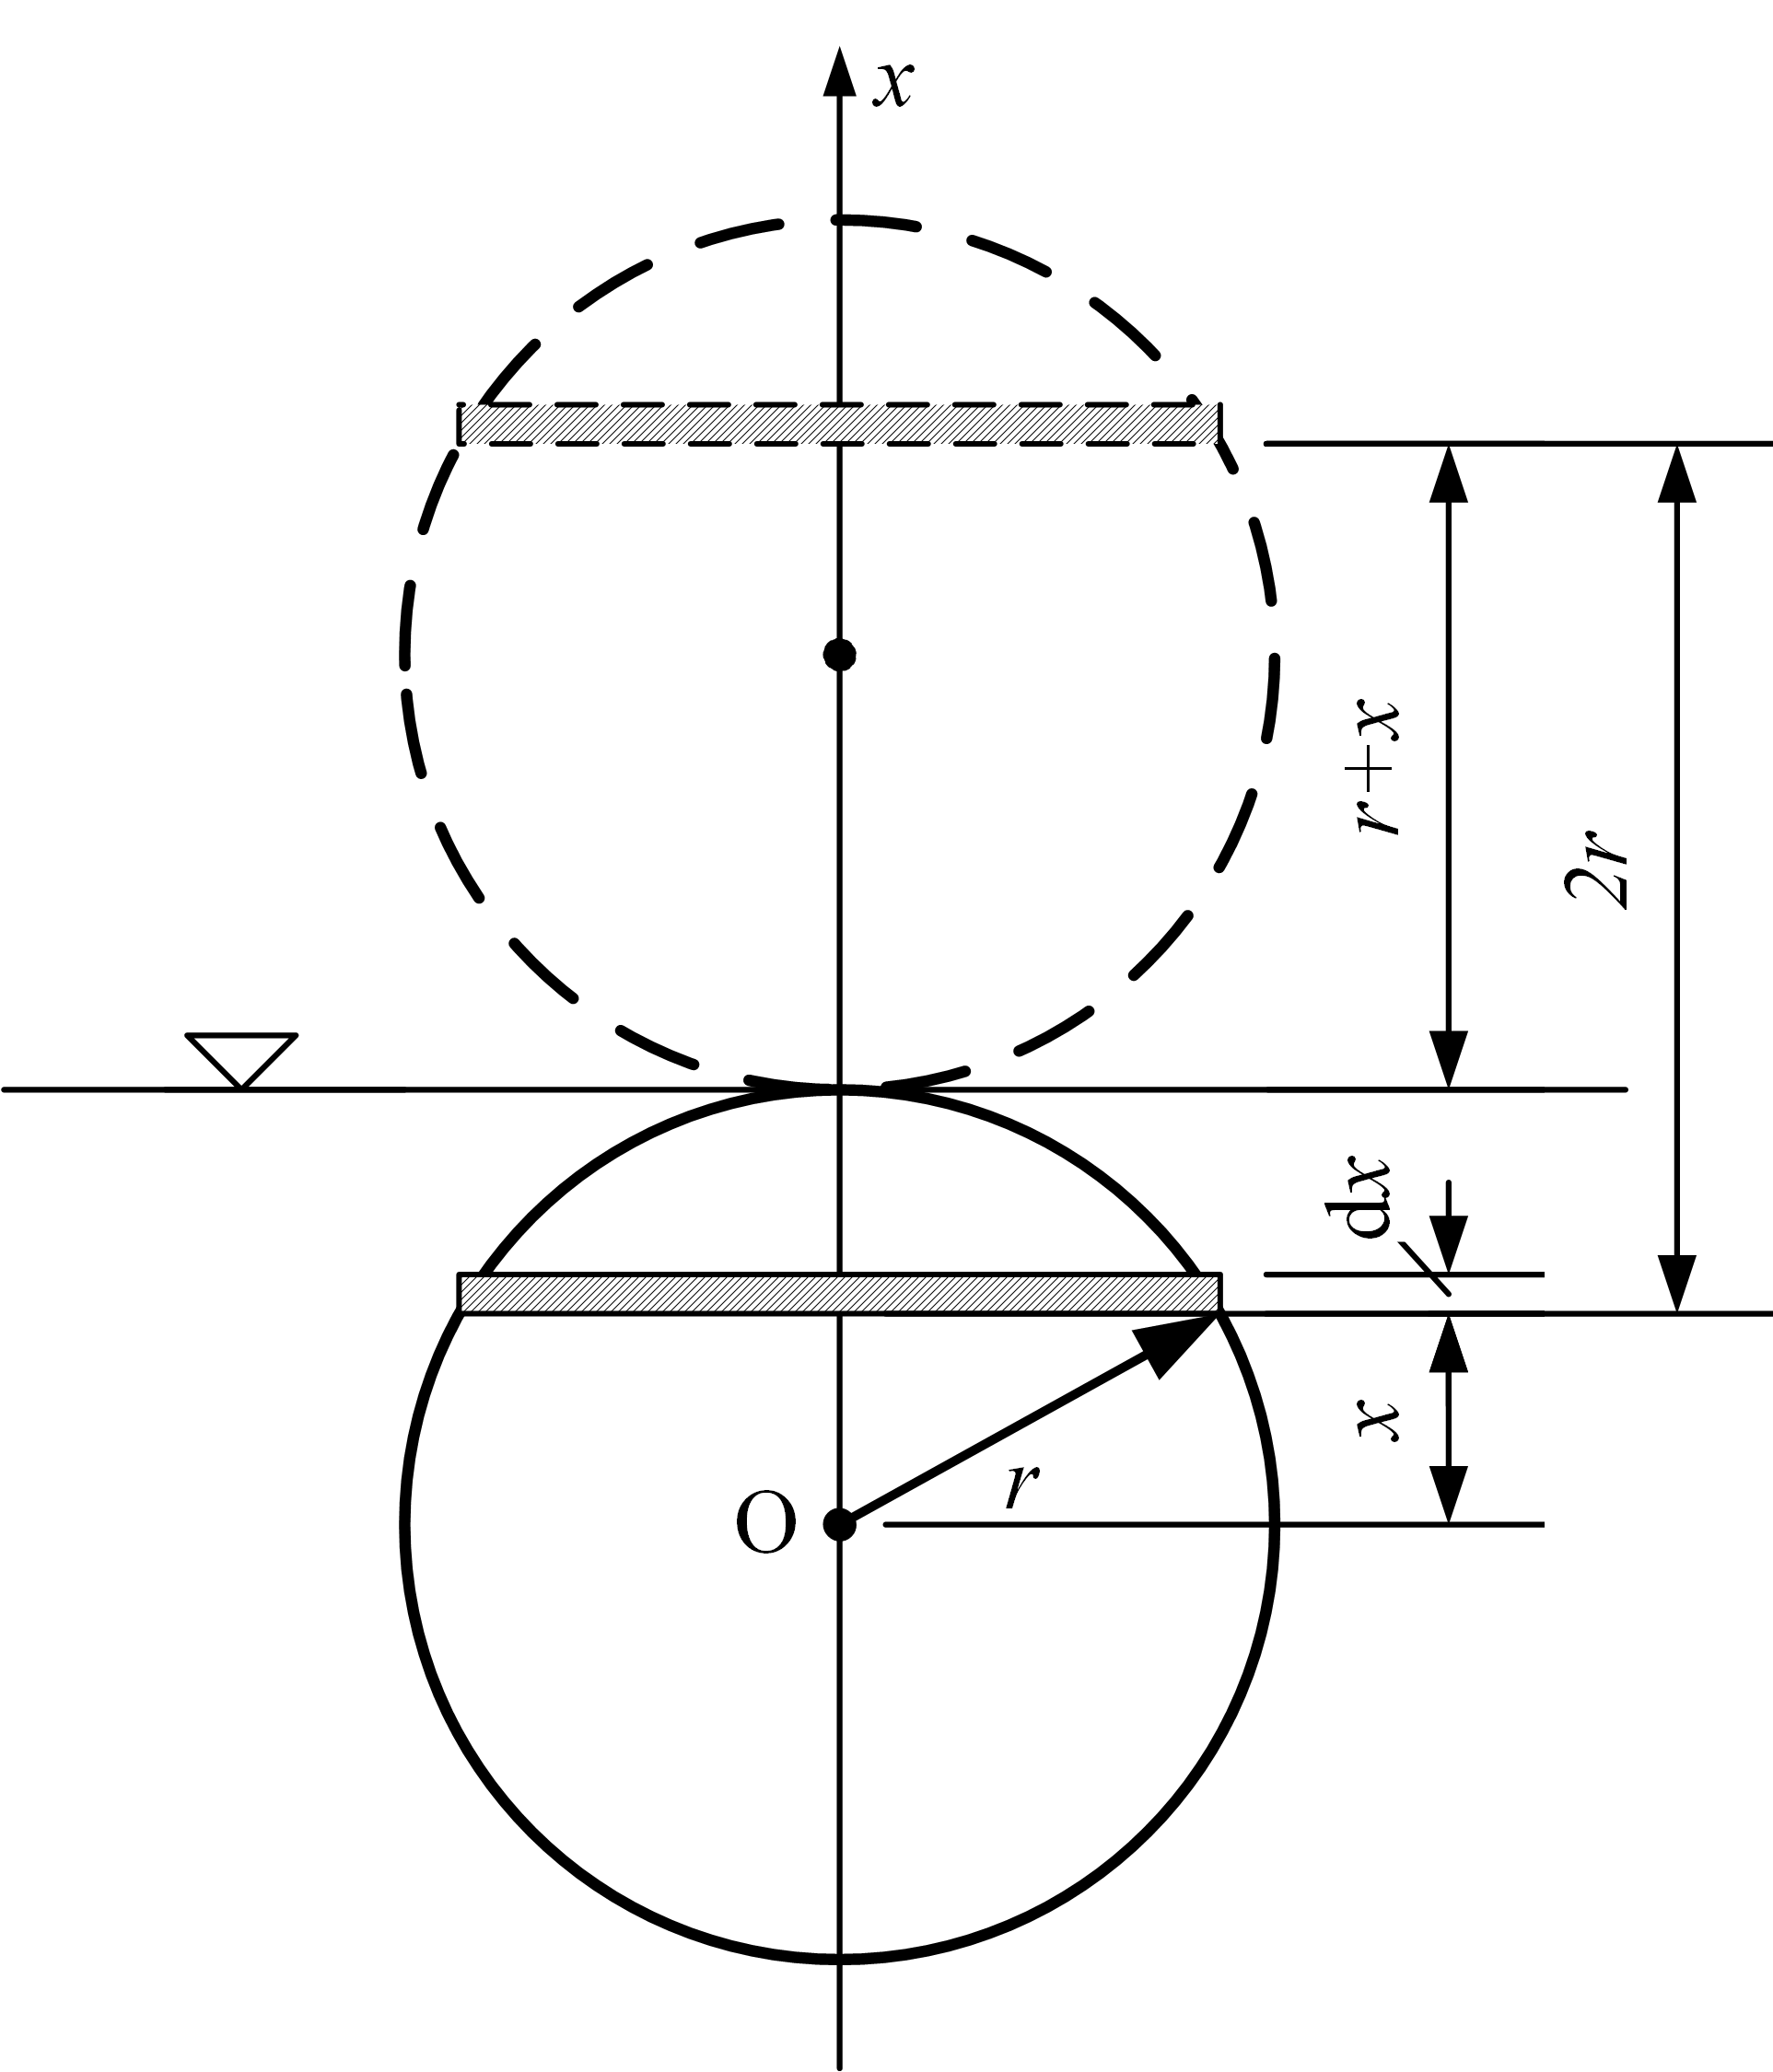
\includegraphics[height=0.3\textheight]{F:/life/2018AutumnTA/Exercises/11/Fig7-6-1.png}
\end{center}
\caption{习题7.6 1.题图示}
\label{7-6-1}
\end{figure}
\item边长等于$1\mathrm m$的质量均匀正立方体,比重为$0.1\mathrm{t/m^3}$. 将其全部压入水中,需要做多少功.

解:方法1:如图~\ref{7-6-2-1}所示,设最初正方体浸入水中部分的深度为$h$,由$\rho_{\text{水}}\mathrm ghL^2=\rho_{\text{正方体}}\mathrm gL^3$得\\
\[h=\frac{\rho_{\text{正方体}}L}{\rho_{\text{水}}}=\frac1{10}L\]
\begin{figure}[H]
\begin{center}
\subfloat[]{\label{7-6-2-1}
{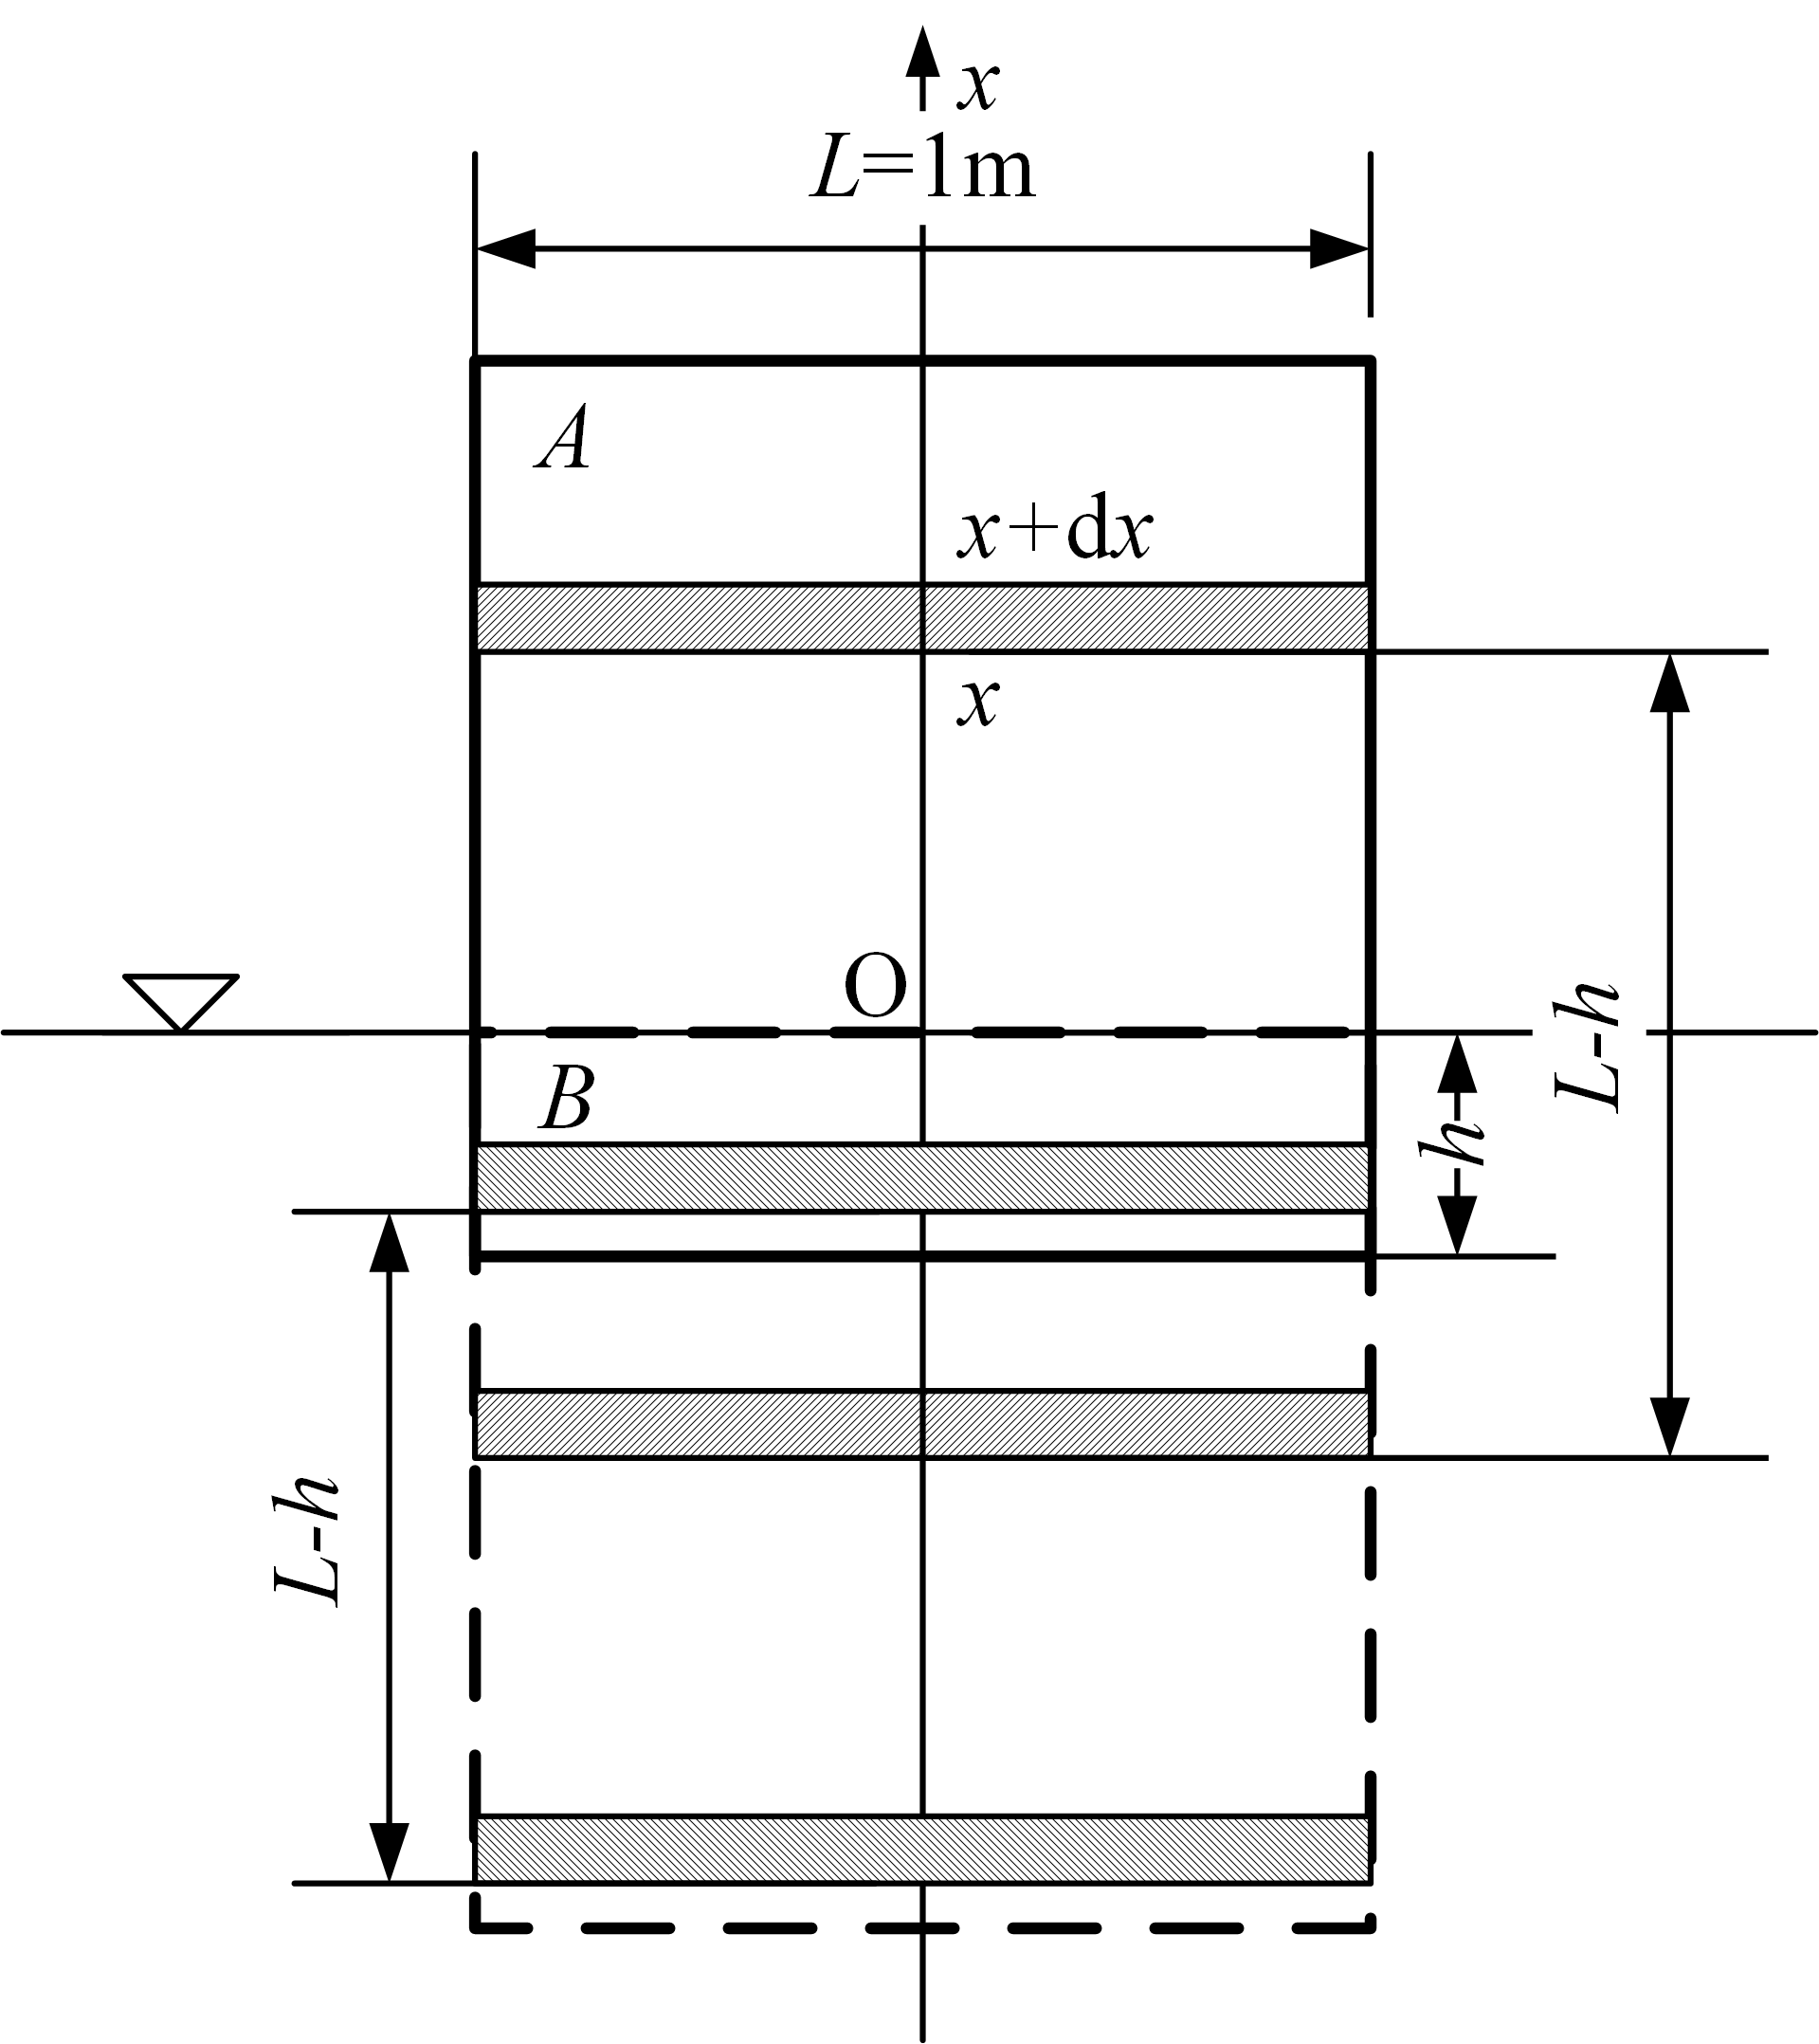
\includegraphics[height=0.3\textheight]{F:/life/2018AutumnTA/Exercises/11/Fig7-6-2-1.png} }}
    \subfloat[]{\label{7-6-2-2} {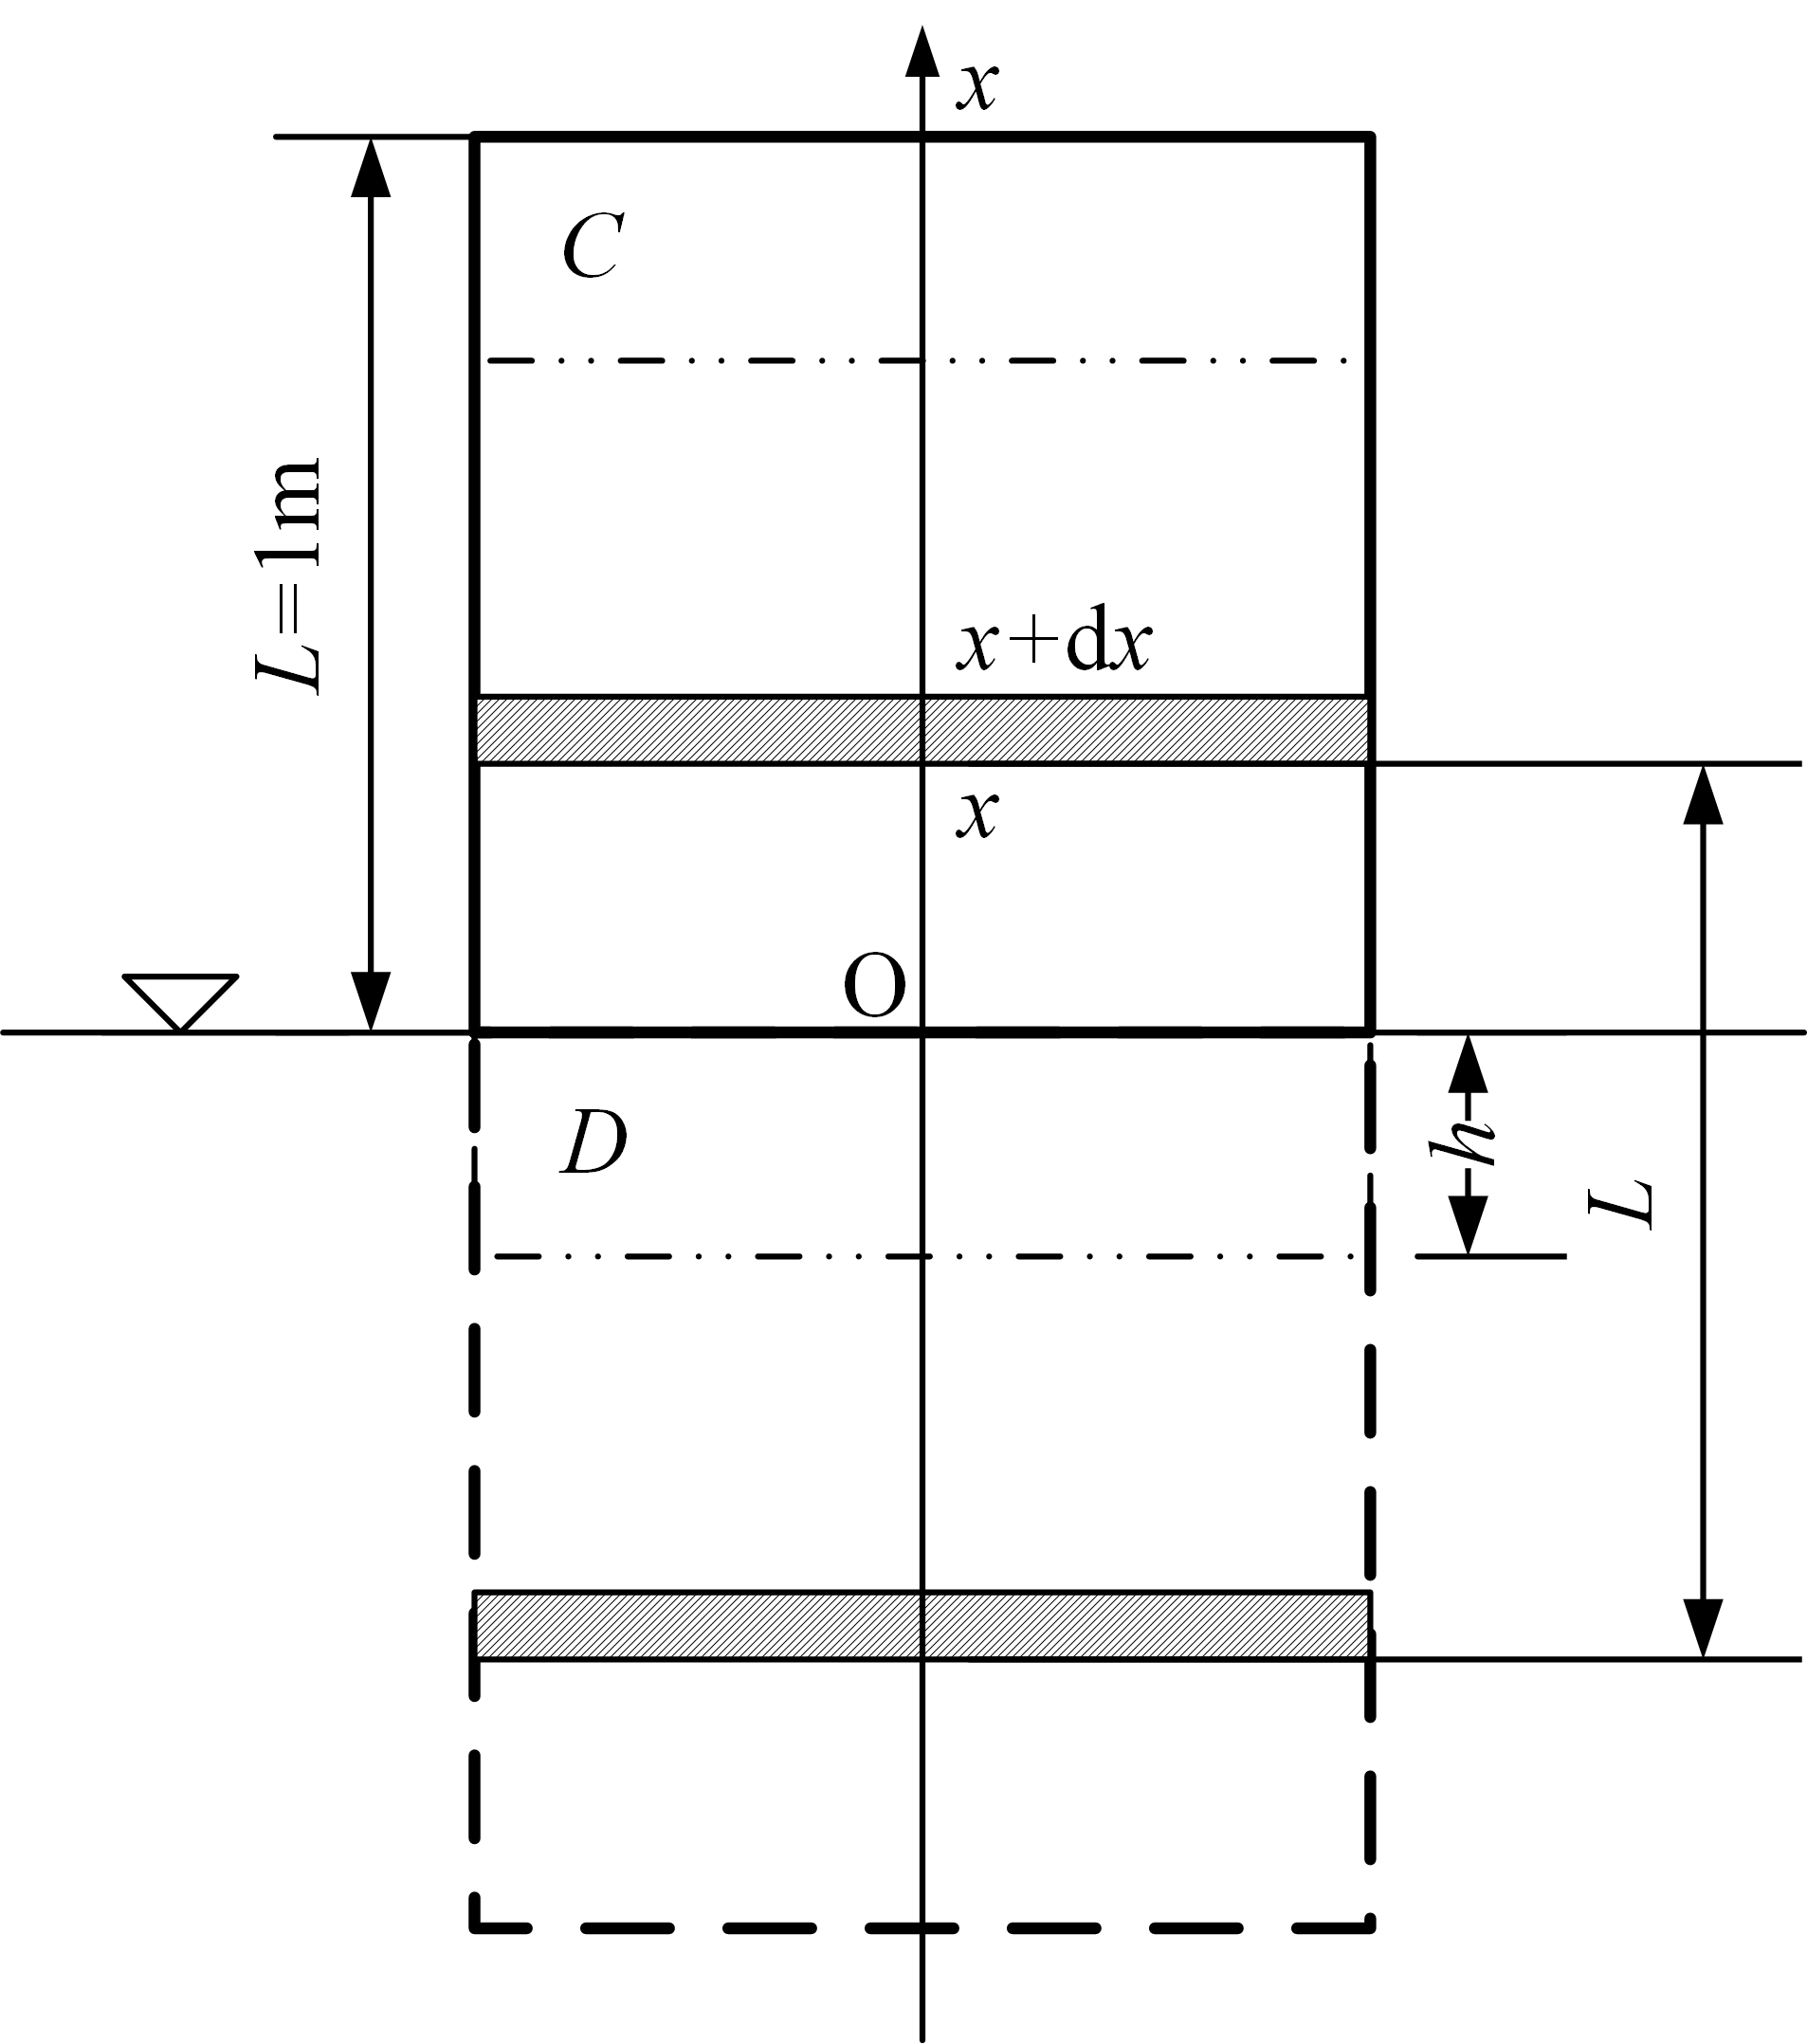
\includegraphics[height=0.3\textheight]{F:/life/2018AutumnTA/Exercises/11/Fig7-6-2-2.png} }}
\end{center}
\caption{习题7.6 2.题图示}
\label{7-6-2}
\end{figure}
可据此将该正方体分为水上部分$A$和水下部分$B$,水上部分$A$处的微元压入水中需做的功
\[\mathrm dW_A=-\rho_{\text{立方体}}\mathrm gL^2\mathrm dx\cdot(L-h)+\rho_{\text{水}}\mathrm gL^2\mathrm dx\cdot(L-h-x)=[-\rho_{\text{立方体}}(L-h)+\rho_{\text{水}}(L-h-x)]\mathrm gL^2\mathrm dx\]
水下部分$B$处的微元压入水中需做的功
\[\mathrm dW_B=-\rho_{\text{立方体}}\mathrm gL^2\mathrm dx\cdot(L-h)+\rho_{\text{水}}\mathrm gL^2\mathrm dx\cdot(L-h)=(-\rho_{\text{立方体}}+\rho_{\text{水}})\mathrm gL^2(L-h)\mathrm dx\]
则将该正方体全部压入水中需要做的功
\[\begin{split}
W&=W_A+W_B=\int_0^{W_A}\mathrm dW_A+\int_0^{W_B}\mathrm dW_B\\
&=\int_0^{L-h}[-\rho_{\text{立方体}}(L-h)+\rho_{\text{水}}(L-h-x)]\mathrm gL^2\mathrm dx+\int_{-h}^0(-\rho_{\text{立方体}}+\rho_{\text{水}})\mathrm gL^2(L-h)\mathrm dx\\
&=\mathrm gL^2[-\rho_{\text{立方体}}(L-h)x+\rho_{\text{水}}(L-h)x-\rho_{\text{水}}\frac12x^2]\Big|_0^{L-h}+(-\rho_{\text{立方体}}+\rho_{\text{水}})\mathrm gL^2(L-h)x\Big|_{-h}^0\\
&=\mathrm gL^2[-\rho_{\text{立方体}}(L-h)^2+\rho_{\text{水}}(L-h)^2-\rho_{\text{水}}\frac12(L-h)^2]+(-\rho_{\text{立方体}}+\rho_{\text{水}})\mathrm gL^2(L-h)h\\
&=\mathrm gL^2(L-h)^2[-\rho_{\text{立方体}}+\rho_{\text{水}}-\frac12\rho_{\text{水}}]+(-\rho_{\text{立方体}}+\rho_{\text{水}})\mathrm gL^2(L-h)h\\
&=\mathrm gL^2(L-h)^2\frac25\rho_{\text{水}}+\frac9{10}\rho_{\text{水}}\mathrm gL^2(L-h)h\\
&=\mathrm gL^2\rho_{\text{水}}[\frac25(L-h)^2+\frac9{10}(L-h)h]\\
&=\mathrm gL^4\rho_{\text{水}}[\frac25(\frac9{10})^2+\frac9{10}\frac9{10}\frac1{10}]\\
&=405\mathrm g(\mathrm J).
\end{split}\]

方法2:如图~\ref{7-6-2-2}所示的微元压入水中需做的功为
\[\mathrm dW=-\rho_{\text{立方体}}\mathrm g\L^2\mathrm dx\cdot L+\rho_{\text{水}}\mathrm gL^2\mathrm dx\cdot(L-x)=[-\rho_{\text{立方体}}L+\rho_{\text{水}}(L-x)]\mathrm g\L^2\mathrm dx\]
设最初正方体下底与水面相平,最初正方体仅在重力的作用下下沉,设稳定后浸入水中部分$D$的深度为$h$,由$\rho_{\text{水}}\mathrm ghL^2=\rho_{\text{正方体}}\mathrm gL^3$得\\
\[h=\frac{\rho_{\text{正方体}}L}{\rho_{\text{水}}}=\frac1{10}L\]
正方体下沉到浸没深度为$h$的过程中外力不做功,相当于将图中立方体的$C$部分转移到$D$部分的过程中外力不做功,外力只对剩余部分做功,故将该正方体全部压入水中需要做的外力功为
\[\begin{split}
W&=\int_0^W\mathrm dW=\int_0^{L-h}[-\rho_{\text{立方体}}L+\rho_{\text{水}}(L-x)]\mathrm g\L^2\mathrm dx\\
&=\mathrm gL^2[-\rho_{\text{立方体}}Lx+\rho_{\text{水}}(Lx-\frac12x^2)]\Big|_0^{L-h}\\
&=\mathrm gL^2[-\rho_{\text{立方体}}L(L-h)+\rho_{\text{水}}L(L-h)-\frac12\rho_{\text{水}}(L-h)^2]\\
&=\mathrm gL^2(L-h)[-\rho_{\text{立方体}}L+\rho_{\text{水}}L-\frac12\rho_{\text{水}}(L-h)]\\
&=\mathrm gL^2\frac9{10}L[-\frac1{10}\rho_{\text{水}}L+\rho_{\text{水}}L-\frac12\rho_{\text{水}}\frac9{10}L]\\
&=\mathrm g\rho_{\text{水}}L^4\frac9{10}\frac9{20}\\
&=405\mathrm g(\mathrm J).
\end{split}\]

\item水库的闸门是等腰梯形,上底$6\mathrm m$,下底$4\mathrm m$,高$10\mathrm m$. 当上底与水面相齐时,求闸门所受的压力.

解:建立如图~\ref{7-6-3}所示的坐标系,图中微元的长度为
\[L=6-2x\tan\theta=6-2x\frac{\frac{6-4}2}{10}=6-\frac15x\]
微元受到的静水压力
\[\mathrm dP=\rho\mathrm gxL\mathrm dx\]
整个闸门受到的静水压力
\[\begin{split}
P&=\int_0^P\mathrm dP=\int_0^{10}\rho\mathrm gxL\mathrm dx=\int_0^{10}\rho\mathrm gx(6-\frac15x)\mathrm dx=\rho\mathrm g(3x^2-\frac1{15}x^3)\Big|_0^{10}=\frac{700}3(\rho\mathrm g=1).
\end{split}\]
\begin{figure}[H]
\begin{center}
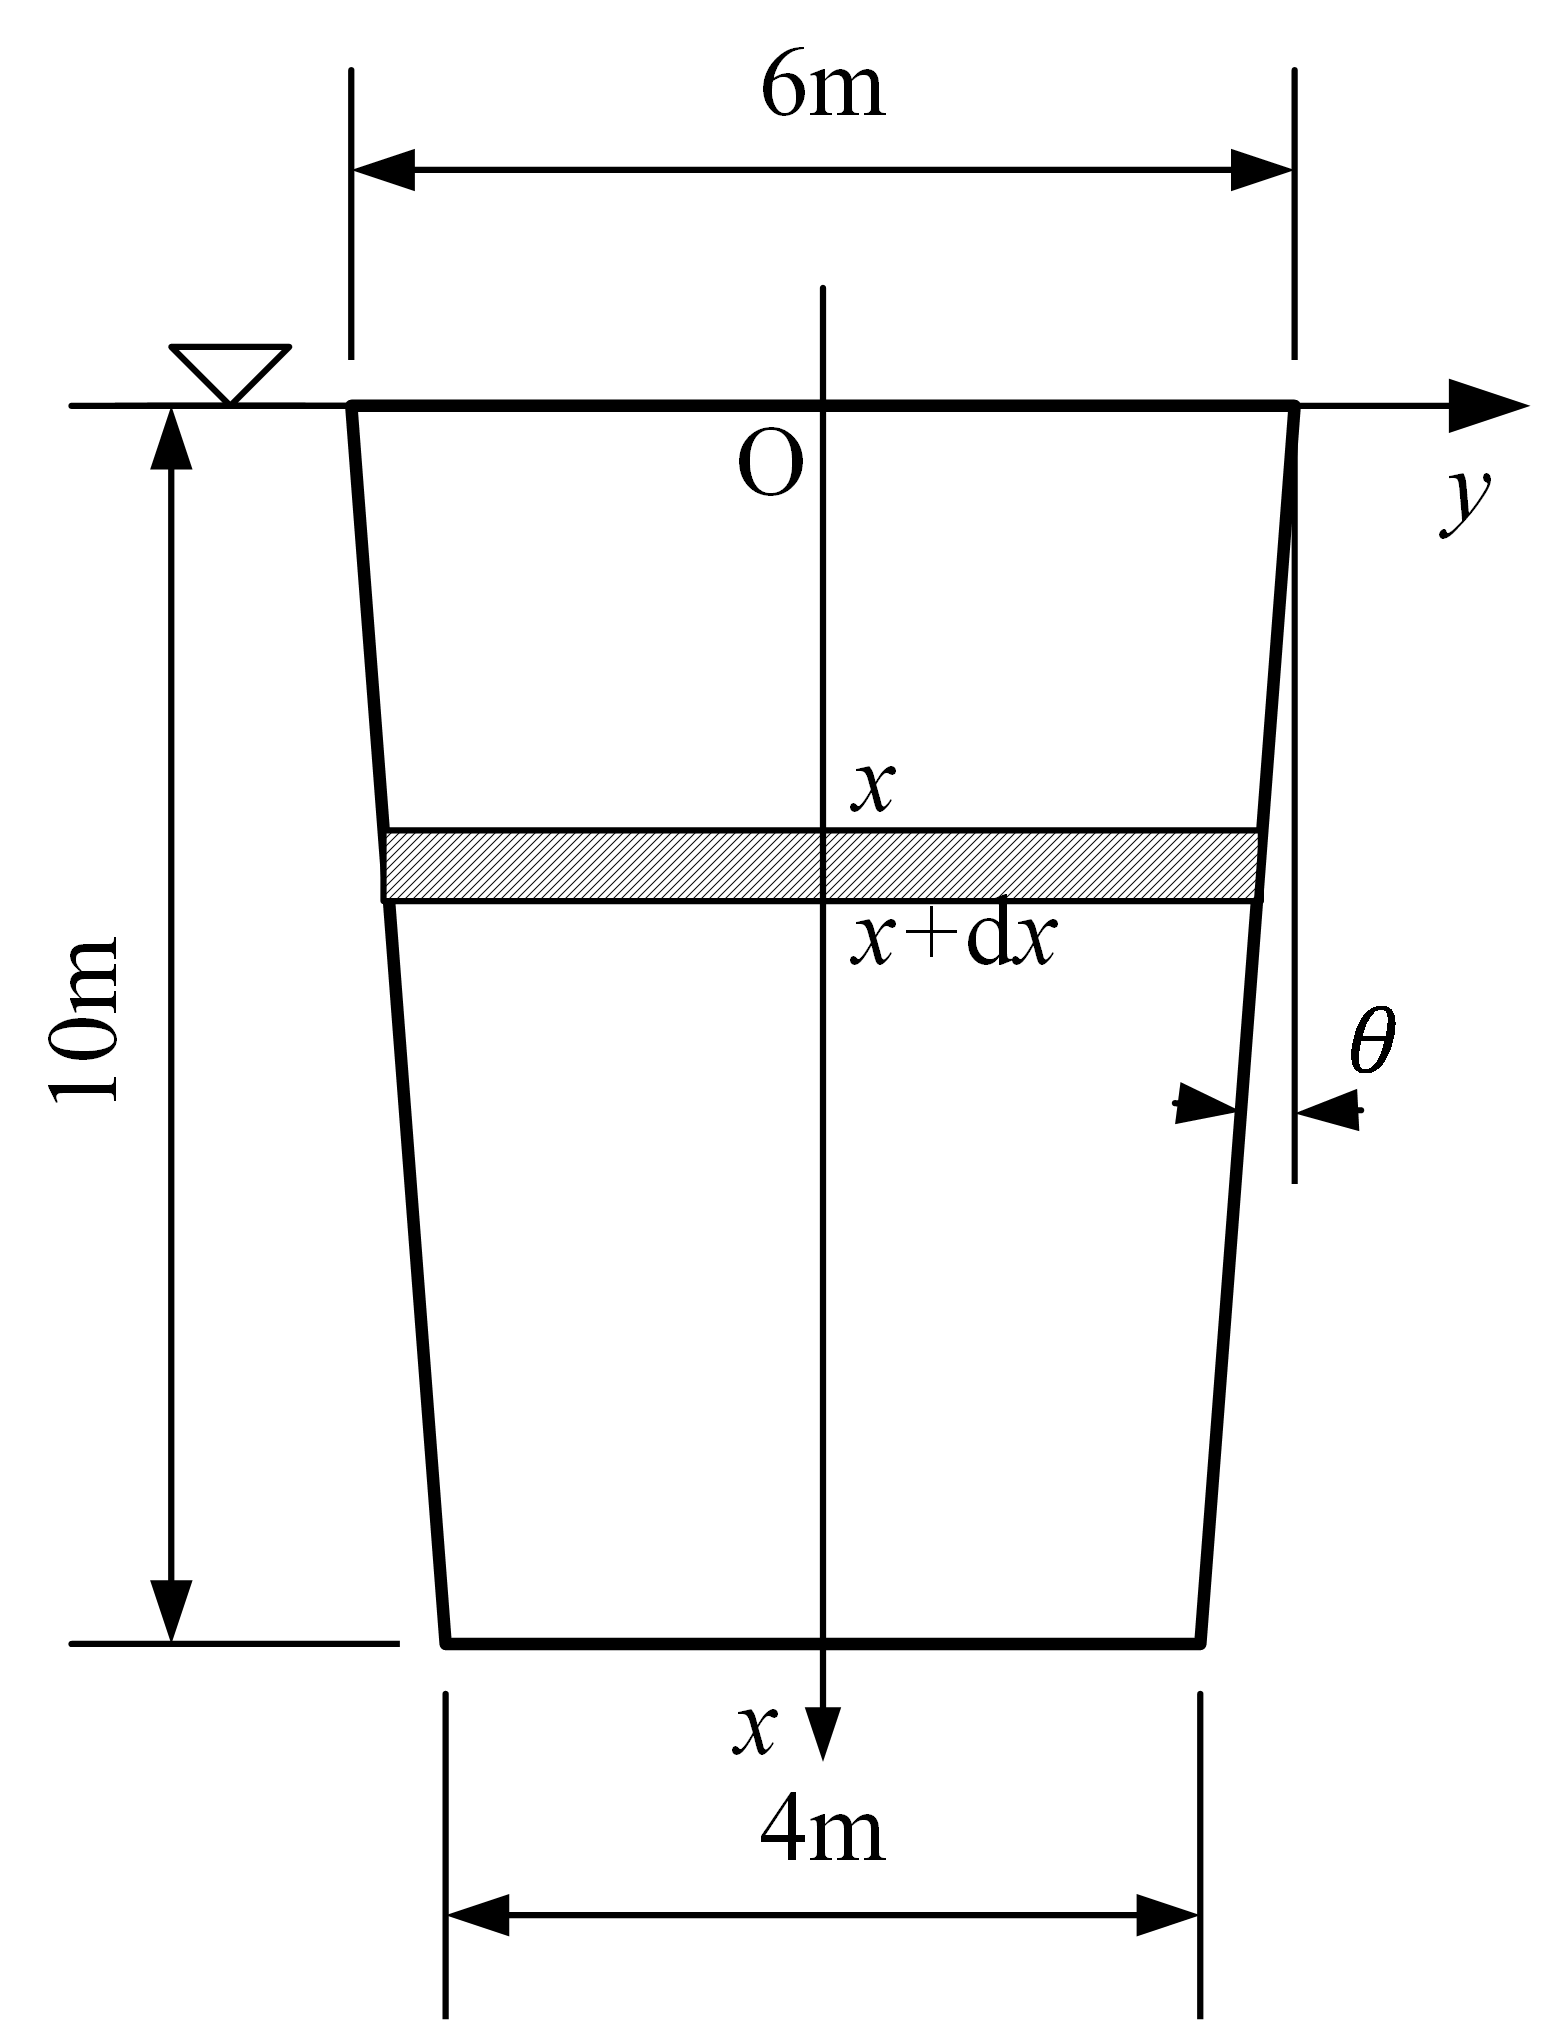
\includegraphics[height=0.3\textheight]{F:/life/2018AutumnTA/Exercises/11/Fig7-6-3.png}
\end{center}
\caption{习题7.6 3.题图示}
\label{7-6-3}
\end{figure}
\item圆形水池直径$20\mathrm m$,高$30\mathrm m$,水深$27\mathrm m$. 如果将水全部抽出,外力要做多少功?

解:建立如图~\ref{7-6-4}所示的坐标系,将图中微元抽出需克服重力做功
\[\mathrm dW=\rho\mathrm g\pi\cdot(\frac{20}2)^2\mathrm dx(30-x)=100\rho\mathrm g\pi(30-x)\mathrm dx\]
外力做的总功
\[W=\int_0^W\mathrm dW=\int_0^{27}100\rho\mathrm g\pi(30-x)\mathrm dx=100\rho\mathrm g\pi(30x-\frac12x^2)\Big|_0^{27}=44550\pi\rho\mathrm g(\mathrm J).\]
\begin{figure}[H]
\begin{center}
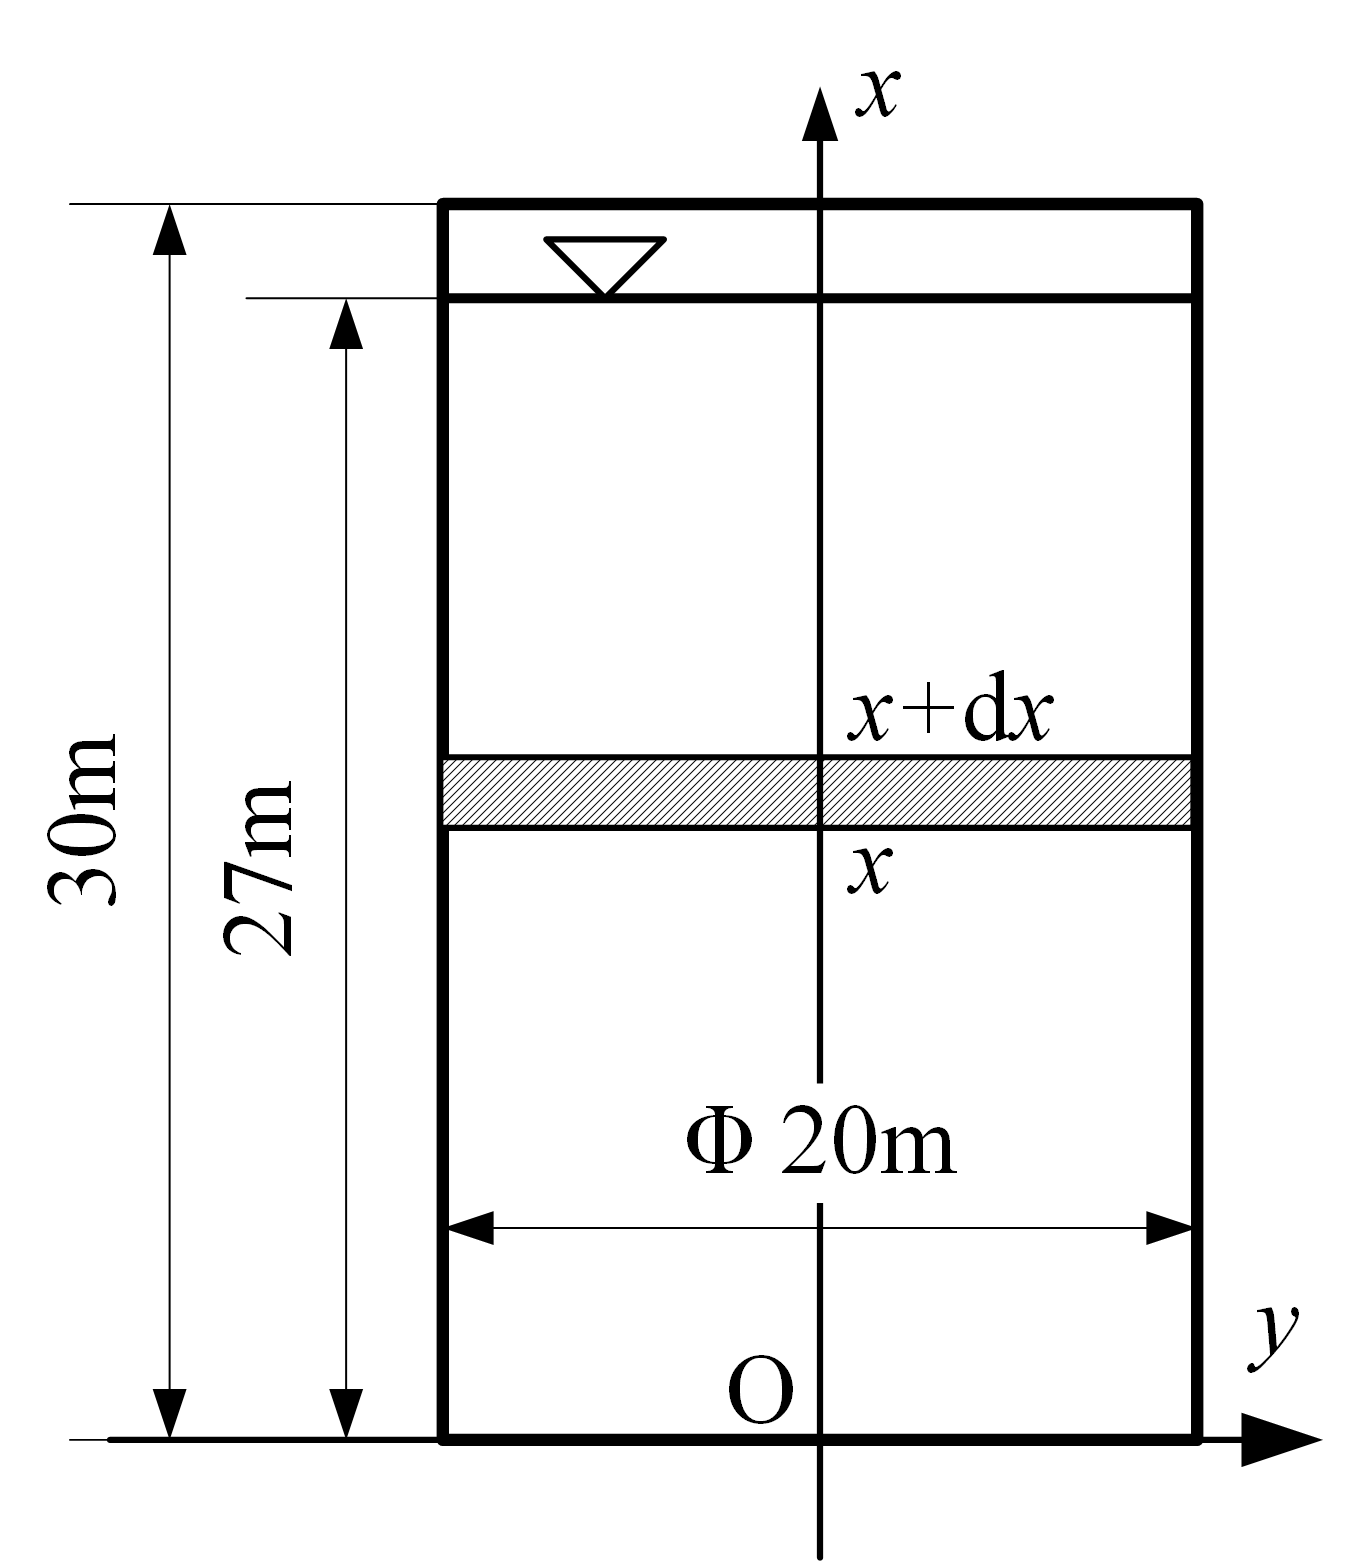
\includegraphics[height=0.3\textheight]{F:/life/2018AutumnTA/Exercises/11/Fig7-6-4.png}
\end{center}
\caption{习题7.6 4.题图示}
\label{7-6-4}
\end{figure}
\item有一个质量为$M$、半径等于$R$的均匀圆周. 在过圆心、且与圆所在平面垂直的直线上距离圆心等于$h$处有一个质量等于$m$的质点. 求圆周对于质点的引力.

解:如图~\ref{7-6-5}所示,取图中所示的质量元,其与关于圆心中心对称的质量元对质点的合力指向圆心,二者对质点在圆周所在平面内的分力$\mathrm dF_x$互相抵消,只需考虑每个质量元对质点指向圆心的分力
\[\mathrm dF_y=\frac{Gm\mathrm dM}{R^2+h^2}\cos\theta=\frac{Gm}{R^2+h^2}\frac h{\sqrt{R^2+h^2}}\mathrm dM\]
整个圆周对质点的引力
\[F=\int_0^F\mathrm dF=\int_0^M\frac{Gm}{R^2+h^2}\frac h{\sqrt{R^2+h^2}}\mathrm dM=\frac{GmMh}{(R^2+h^2)^{\frac32}}=\frac{Mmh}{(R^2+h^2)^{\frac32}}(G=1).\]
\begin{figure}[H]
\begin{center}
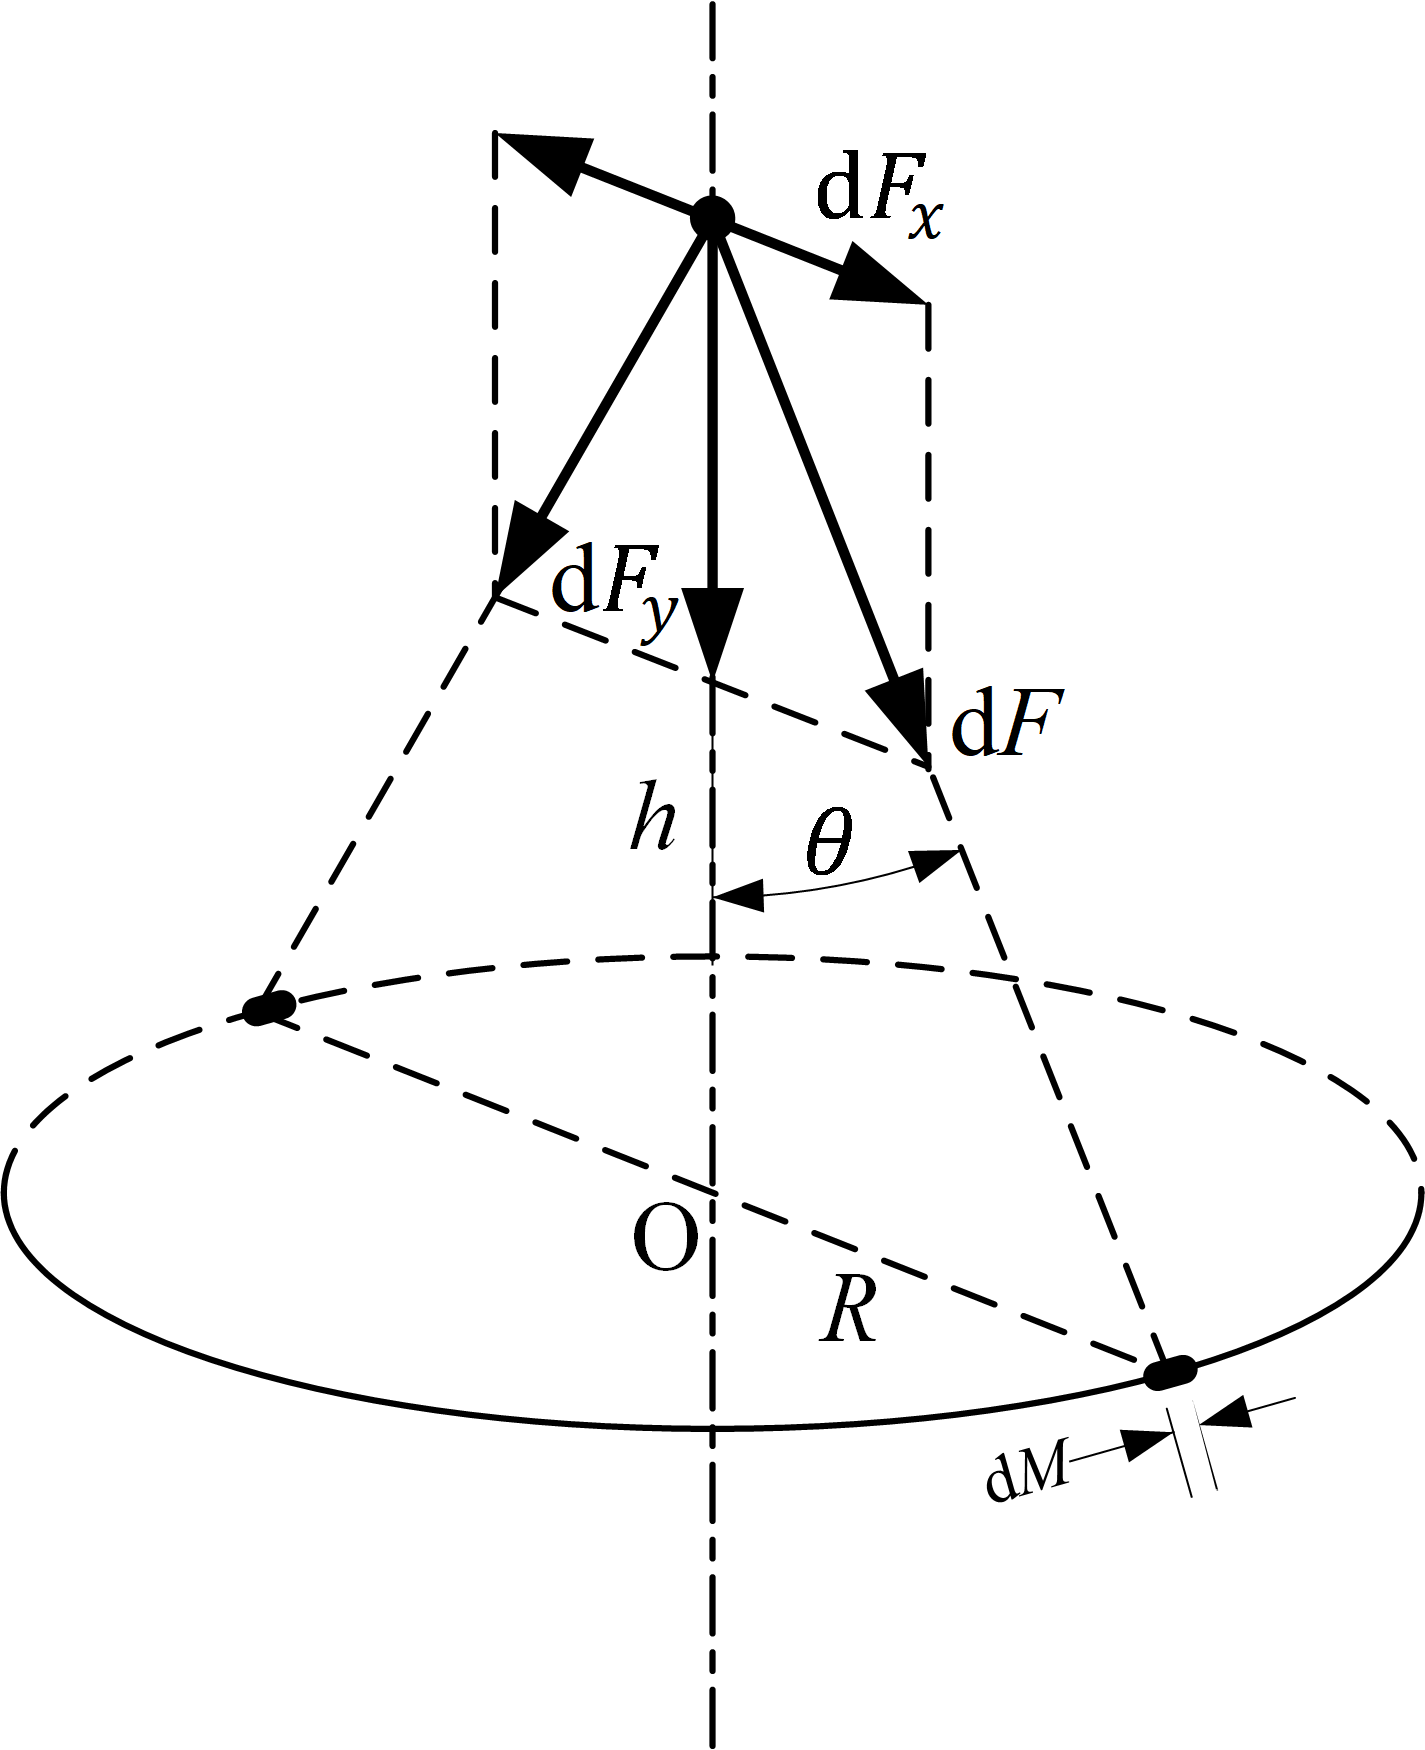
\includegraphics[height=0.3\textheight]{F:/life/2018AutumnTA/Exercises/11/Fig7-6-5.png}
\end{center}
\caption{习题7.6 5.题图示}
\label{7-6-5}
\end{figure}
\item设$2\mathrm{kg}$的力能使弹簧伸长$1\mathrm{cm}$. 求使弹簧伸长$1\mathrm m$需要做的功.

解:弹簧常数$k=\frac{m\mathrm g}{\Delta x}=\frac{2\mathrm g}{0.01}=200\mathrm g$

使弹簧伸长$1\mathrm m$需要做功$W=\int_0^1kx\mathrm dx=\frac12kx^2\Big|_0^1=\frac12\times200\mathrm g=100\mathrm g(\mathrm J).$
\end{enumerate}
\subsection{习题7.7解答}
\begin{enumerate}
\item计算下列反常积分:
\newline
\begin{tabular}{ll}
(1)$\int_2^{+\infty}\frac{\mathrm dx}{x^2-1}$;&(2)$\int_1^{+\infty}\frac{\arctan x}{x^3}\mathrm dx$;\\
(3)$\int_0^{+\infty}x\mathrm e^{-x^2}\mathrm dx$;&(4)$\int_{\mathrm e}^{+\infty}\frac{\mathrm dx}{x(\ln x)^2}$;\\
(5)$\int_1^{+\infty}\frac{\mathrm dx}{x\sqrt{x^2-1}}$;&(6)$\int_0^1\frac{\arcsin x}{\sqrt{1-x^2}}\mathrm dx$;\\
(7)$\int_0^1\ln x\mathrm dx$;&(8)$\int_1^{\mathrm e}\frac{\mathrm dx}{x\sqrt{1-(\ln x)^2}}$.
\end{tabular}

解:(1)$\int_2^{+\infty}\frac{\mathrm dx}{x^2-1}=\frac12\int_2^{+\infty}(\frac1{x-1}-\frac1{x+1})=\frac12\ln|\frac{x-1}{x+1}|\Big|_2^{+\infty}=-\frac12\ln\frac13=\frac12\ln3$.

(2)$\int_1^{+\infty}\frac{\arctan x}{x^3}\mathrm dx=\int_1^{+\infty}\arctan x\mathrm d(-\frac1{2x^2})=-\frac{\arctan x}{x^2}\Big|_1^{+\infty}+\int_1^{+\infty}\frac1{x^2}\mathrm d\arctan x\\
=\frac\pi4+\int_1^{+\infty}\frac1{x^2(1+x^2)}\mathrm dx=-\frac\pi4+\int_1^{+\infty}(\frac1{x^2}-\frac1{1+x^2})\mathrm dx=\frac\pi4+(-\frac1x-\arctan x)\Big|_1^{+\infty}\\
=\frac\pi4+[1-(\frac\pi2-\frac\pi4)]=1$.

(3)$\int_0^{+\infty}x\mathrm e^{-x^2}\mathrm dx=-\frac12\int_0^{+\infty}\mathrm e^{-x^2}\mathrm d(-x^2)=\mathrm e^{-x^2}\Big|_0^{+\infty}=-1$.

(4)$\int_{\mathrm e}^{+\infty}\frac{\mathrm dx}{x(\ln x)^2}=\int_{\mathrm e}^{+\infty}\frac1{(\ln x)^2}\mathrm d\ln x=-\frac1{\ln x}\Big|_{\mathrm e}^{+\infty}=1$.

(5)$\int_1^{+\infty}\frac{\mathrm dx}{x\sqrt{x^2-1}}\xlongequal{x=\sec t}\int_0^{\frac\pi2}\frac{\sec t\tan t\mathrm dt}{\sec t\tan t}=\frac\pi2$.

(6)$\int_0^1\frac{\arcsin x}{\sqrt{1-x^2}}\mathrm dx=\int_0^1\arcsin x\mathrm d\arcsin x=\frac12\arcsin^2x\Big|_0^1=\frac{\pi^2}8$.

(7)$\int_0^1\ln x\mathrm dx=x\ln x\Big|_0^1-\int_0^1x\mathrm d\ln x=-\int_0^1x\frac1x\mathrm dx=-1$.

(8)$\int_1^{\mathrm e}\frac{\mathrm dx}{x\sqrt{1-(\ln x)^2}}=\int_1^{\mathrm e}\frac{\mathrm d\ln x}{\sqrt{1-(\ln x)^2}}=\arcsin(\ln x)\Big|_1^{\mathrm e}=\frac\pi2$.
\item讨论下列广义积分的收敛性:
\newline
\begin{tabular}{ll}
(1)$\int_0^{+\infty}\frac{x^2}{x^4-x^2+1}\mathrm dx$;&(2)$\int_0^{+\infty}\frac{x^m}{1+x^n}\mathrm dx,m>0,n>0$;\\
(3)$\int_0^{+\infty}x^n\mathrm e^{-x}\mathrm dx,n>0$;&(4)$\int_1^{+\infty}\frac{\mathrm dx}{x^p+x^q},p>0,q>0$;\\
(5)$\int_0^1x^a\ln x\mathrm dx,a>0$;&(6)$\int_0^1\frac{\ln x}{1-x}\mathrm dx$;\\
\multicolumn{2}{l}{(7)$\int_0^{\frac\pi2}\frac{\mathrm dx}{\sin^px\cos^qx},p>0,q>0$;}\\
\multicolumn{2}{l}{(8)$\int_0^1x^{p-1}(1-x)^{q-1}\ln x\mathrm dx$.}
\end{tabular}

解:(1)$\because\lim\limits_{x\rightarrow+\infty}x^2\cdot\frac{x^2}{x^4-x^3+1}=1$

$\therefore\int_0^{+\infty}\frac{x^2}{x^4-x^2+1}\mathrm dx$收敛.

(2)$\because\lim\limits_{x\rightarrow+\infty}x^{n-m}\cdot\frac{x^m}{1+x^n}=\lim\limits_{x\rightarrow+\infty}\frac{x^n}{1+x^n}=1$

$\therefore$当$n-m>1$时,$\int_0^{+\infty}\frac{x^m}{1+x^n}\mathrm dx$收敛,当$n-m\leq1$时$\int_0^{+\infty}\frac{x^m}{1+x^n}\mathrm dx$发散.

(3)$\because\lim\limits_{x\rightarrow+\infty}x^2\cdot x^n\mathrm e^{-x}=\lim\limits_{x\rightarrow+\infty}\frac{x^{n+2}}{\mathrm e^x}=0$

$\therefore\int_0^{+\infty}x^n\mathrm e^{-x}\mathrm dx$收敛.

(4)不妨设$p\geq q$,$\lim\limits_{x\rightarrow+\infty}x^p\cdot\frac1{x^p+x^q}=\begin{cases}
1,&p>q\\
\frac12,&p=q
\end{cases}$

i)当$p>1$或$q>1$时,$\int_1^{+\infty}\frac{\mathrm dx}{x^p+x^q}$收敛;

ii)当$p\leq1$且$q\leq1$时,$\int_1^{+\infty}\frac{\mathrm dx}{x^p+x^q}$发散.

(5)$\because\lim\limits_{x\rightarrow0^+}x^{\frac12}\cdot|x^a\ln x|=-\lim\limits_{x\rightarrow0^+}x^{\frac12+a}\ln x=0$

$\therefore\int_0^1x^a\ln x\mathrm dx$收敛.

(6)$\int_0^1\frac{\ln x}{1-x}\mathrm dx=\int_0^{\frac12}\frac{\ln x}{1-x}\mathrm dx+\int_{\frac12}^1\frac{\ln x}{1-x}\mathrm dx=I_1+I_2$

$\because\lim\limits_{x\rightarrow0^+}x^{\frac12}\cdot|\frac{\ln x}{1-x}|=-\lim\limits_{x\rightarrow0^+}x^{\frac12}\cdot\frac{\ln x}{1-x}=0$,故$I_1$收敛;

$\because\lim\limits_{x\rightarrow1^-}(1-x)^{\frac12}\cdot|\frac{\ln x}{1-x}|=-\lim\limits_{x\rightarrow1^-}(1-x)^{\frac12}\cdot\frac{\ln[1-(1-x)]}{1-x}=-\lim\limits_{x\rightarrow1^-}(1-x)^{\frac12}\cdot(-1)=0$,故$I_2$收敛;

综上所述,$\int_0^1\frac{\ln x}{1-x}\mathrm dx$收敛.

(7)$\int_0^{\frac\pi2}\frac{\mathrm dx}{\sin^px\cos^qx}=\int_0^{\frac\pi4}\frac{\mathrm dx}{\sin^px\cos^qx}+\int_{\frac\pi4}^{\frac\pi2}\frac{\mathrm dx}{\sin^px\cos^qx}=I_1+I_2$

$\because\lim\limits_{x\rightarrow0^+}x^p\cdot\frac1{\sin^px\cos^qx}=\frac{x^p}{\sin^px}\frac1{\cos^qx}=1$

$\therefore$当$p<1$时$I_1$收敛,当$p\geq1$时$I_1$发散;

$\because\lim\limits_{x\rightarrow\frac\pi2^-}(\frac\pi2-x)^q\cdot\frac1{\sin^px\cos^qx}=\lim\limits_{x\rightarrow\frac\pi2^-}\frac1{\sin^px}\frac{(\frac\pi2-x)^q}{\sin^q(\frac\pi2-x)}=1$

$\therefore$当$q<1$时$I_2$收敛,当$q\geq1$时$I_2$发散;

综上所述,当$p<1$且$q<1$时$\int_0^{\frac\pi2}\frac{\mathrm dx}{\sin^px\cos^qx}$收敛,否则发散.

(8)$\int_0^1x^{p-1}(1-x)^{q-1}\ln x\mathrm dx=\int_0^{\frac12}x^{p-1}(1-x)^{q-1}\ln x\mathrm dx+\int_{\frac12}^1x^{p-1}(1-x)^{q-1}\ln x\mathrm dx=I_1+I_2$

i)$\lim\limits_{x\rightarrow0^+}x^a\cdot|x^{p-1}(1-x)^{q-1}\ln x|=-\lim\limits_{x\rightarrow0^+}(1-x)^{q-1}x^{a+p-1}\ln x=\begin{cases}
0,&a+p-1>0\\
+\infty,&a+p-1\leq0
\end{cases}$

\textcircled{1}当$1-p<1$,即$p>0$时,取$a=\frac{1-p+1}2=\frac{2-p}2<1$,则$a+p-1=\frac p2>0$,$I_1$收敛,

\textcircled{2}当$1-p\geq1$,即$p\leq0$时,取$a=\frac{1-p+1}2=\frac{2-p}2\geq1$,则$a+p-1=\frac p2\leq0$,$I_1$发散;

ii)$\lim\limits_{x\rightarrow1^-}(1-x)^b\cdot|x^{p-1}(1-x)^{q-1}\ln x|=-\lim\limits_{x\rightarrow1^-}x^{p-1}(1-x)^{b+q-1}\ln[1-(1-x)]\\
=-\lim\limits_{x\rightarrow1^-}x^{p-1}(1-x)^{b+q-1}[-(1-x)]=\lim\limits_{x\rightarrow1^-}x^{p-1}(1-x)^{b+q}=\begin{cases}
0,&b+q>0\\
1,&b+q=0\\
+\infty,&b+q<0
\end{cases}$

\textcircled{1}当$-q<1$,即$q>-1$时,取$b=\frac{-q+1}2=\frac{1-q}2<1$,则$b+q=\frac{q+1}2>0$,$I_2$收敛,

\textcircled{2}当$-q\geq1$,即$q\leq-1$时,取$b=\frac{-q+1}2=\frac{1-q}2\geq1$,则$b+q=\frac{q+1}2\leq0$,$I_2$发散;

综上所述,当$p>0$且$q>-1$时,$\int_0^1x^{p-1}(1-x)^{q-1}\ln x\mathrm dx$收敛,否则发散.

\item设$f(x),g(x)$在任意区间$[0,A]$上可积$(A>0)$,且$\int_0^{+\infty}f^2(x)\mathrm dx,\int_0^{+\infty}g^2(x)\mathrm dx$都收敛,试证:
\newline
(1)$\int_0^{+\infty}f(x)g(x)\mathrm dx$绝对收敛,即$\int_0^{+\infty}|f(x)g(x)|\mathrm dx$收敛;
\newline
(2)$\int_0^{+\infty}(f(x)+g(x))^2\mathrm dx$收敛.

证明:(1)$\because0\leq|f(x)g(x)|\leq\frac{f^2(x)+g^2(x)}2,x\in[0,A],A>0$

又$\because\int_0^{+\infty}f^2(x)\mathrm dx,\int_0^{+\infty}g^2(x)\mathrm dx$都收敛

$\therefore\int_0^{+\infty}\frac{f^2(x)+g^2(x)}2\mathrm dx$收敛

$\therefore\int_0^{+\infty}|f(x)g(x)|\mathrm dx$收敛

$\therefore\int_0^{+\infty}f(x)g(x)\mathrm dx$绝对收敛.

(2)$\because\int_0^{+\infty}f(x)g(x)\mathrm dx$绝对收敛

$\therefore\int_0^{+\infty}f(x)g(x)\mathrm dx$收敛

$\therefore\int_0^{+\infty}(f(x)+g(x))^2\mathrm dx=\int_0^{+\infty}(f^2(x)+2f(x)g(x)+g^2(x))\mathrm dx$收敛.
\end{enumerate}
\end{document}